% Options for packages loaded elsewhere
\PassOptionsToPackage{unicode}{hyperref}
\PassOptionsToPackage{hyphens}{url}
%
\documentclass[
]{book}
\usepackage{amsmath,amssymb}
\usepackage{iftex}
\ifPDFTeX
  \usepackage[T1]{fontenc}
  \usepackage[utf8]{inputenc}
  \usepackage{textcomp} % provide euro and other symbols
\else % if luatex or xetex
  \usepackage{unicode-math} % this also loads fontspec
  \defaultfontfeatures{Scale=MatchLowercase}
  \defaultfontfeatures[\rmfamily]{Ligatures=TeX,Scale=1}
\fi
\usepackage{lmodern}
\ifPDFTeX\else
  % xetex/luatex font selection
\fi
% Use upquote if available, for straight quotes in verbatim environments
\IfFileExists{upquote.sty}{\usepackage{upquote}}{}
\IfFileExists{microtype.sty}{% use microtype if available
  \usepackage[]{microtype}
  \UseMicrotypeSet[protrusion]{basicmath} % disable protrusion for tt fonts
}{}
\makeatletter
\@ifundefined{KOMAClassName}{% if non-KOMA class
  \IfFileExists{parskip.sty}{%
    \usepackage{parskip}
  }{% else
    \setlength{\parindent}{0pt}
    \setlength{\parskip}{6pt plus 2pt minus 1pt}}
}{% if KOMA class
  \KOMAoptions{parskip=half}}
\makeatother
\usepackage{xcolor}
\usepackage{color}
\usepackage{fancyvrb}
\newcommand{\VerbBar}{|}
\newcommand{\VERB}{\Verb[commandchars=\\\{\}]}
\DefineVerbatimEnvironment{Highlighting}{Verbatim}{commandchars=\\\{\}}
% Add ',fontsize=\small' for more characters per line
\usepackage{framed}
\definecolor{shadecolor}{RGB}{248,248,248}
\newenvironment{Shaded}{\begin{snugshade}}{\end{snugshade}}
\newcommand{\AlertTok}[1]{\textcolor[rgb]{0.94,0.16,0.16}{#1}}
\newcommand{\AnnotationTok}[1]{\textcolor[rgb]{0.56,0.35,0.01}{\textbf{\textit{#1}}}}
\newcommand{\AttributeTok}[1]{\textcolor[rgb]{0.13,0.29,0.53}{#1}}
\newcommand{\BaseNTok}[1]{\textcolor[rgb]{0.00,0.00,0.81}{#1}}
\newcommand{\BuiltInTok}[1]{#1}
\newcommand{\CharTok}[1]{\textcolor[rgb]{0.31,0.60,0.02}{#1}}
\newcommand{\CommentTok}[1]{\textcolor[rgb]{0.56,0.35,0.01}{\textit{#1}}}
\newcommand{\CommentVarTok}[1]{\textcolor[rgb]{0.56,0.35,0.01}{\textbf{\textit{#1}}}}
\newcommand{\ConstantTok}[1]{\textcolor[rgb]{0.56,0.35,0.01}{#1}}
\newcommand{\ControlFlowTok}[1]{\textcolor[rgb]{0.13,0.29,0.53}{\textbf{#1}}}
\newcommand{\DataTypeTok}[1]{\textcolor[rgb]{0.13,0.29,0.53}{#1}}
\newcommand{\DecValTok}[1]{\textcolor[rgb]{0.00,0.00,0.81}{#1}}
\newcommand{\DocumentationTok}[1]{\textcolor[rgb]{0.56,0.35,0.01}{\textbf{\textit{#1}}}}
\newcommand{\ErrorTok}[1]{\textcolor[rgb]{0.64,0.00,0.00}{\textbf{#1}}}
\newcommand{\ExtensionTok}[1]{#1}
\newcommand{\FloatTok}[1]{\textcolor[rgb]{0.00,0.00,0.81}{#1}}
\newcommand{\FunctionTok}[1]{\textcolor[rgb]{0.13,0.29,0.53}{\textbf{#1}}}
\newcommand{\ImportTok}[1]{#1}
\newcommand{\InformationTok}[1]{\textcolor[rgb]{0.56,0.35,0.01}{\textbf{\textit{#1}}}}
\newcommand{\KeywordTok}[1]{\textcolor[rgb]{0.13,0.29,0.53}{\textbf{#1}}}
\newcommand{\NormalTok}[1]{#1}
\newcommand{\OperatorTok}[1]{\textcolor[rgb]{0.81,0.36,0.00}{\textbf{#1}}}
\newcommand{\OtherTok}[1]{\textcolor[rgb]{0.56,0.35,0.01}{#1}}
\newcommand{\PreprocessorTok}[1]{\textcolor[rgb]{0.56,0.35,0.01}{\textit{#1}}}
\newcommand{\RegionMarkerTok}[1]{#1}
\newcommand{\SpecialCharTok}[1]{\textcolor[rgb]{0.81,0.36,0.00}{\textbf{#1}}}
\newcommand{\SpecialStringTok}[1]{\textcolor[rgb]{0.31,0.60,0.02}{#1}}
\newcommand{\StringTok}[1]{\textcolor[rgb]{0.31,0.60,0.02}{#1}}
\newcommand{\VariableTok}[1]{\textcolor[rgb]{0.00,0.00,0.00}{#1}}
\newcommand{\VerbatimStringTok}[1]{\textcolor[rgb]{0.31,0.60,0.02}{#1}}
\newcommand{\WarningTok}[1]{\textcolor[rgb]{0.56,0.35,0.01}{\textbf{\textit{#1}}}}
\usepackage{longtable,booktabs,array}
\usepackage{calc} % for calculating minipage widths
% Correct order of tables after \paragraph or \subparagraph
\usepackage{etoolbox}
\makeatletter
\patchcmd\longtable{\par}{\if@noskipsec\mbox{}\fi\par}{}{}
\makeatother
% Allow footnotes in longtable head/foot
\IfFileExists{footnotehyper.sty}{\usepackage{footnotehyper}}{\usepackage{footnote}}
\makesavenoteenv{longtable}
\usepackage{graphicx}
\makeatletter
\def\maxwidth{\ifdim\Gin@nat@width>\linewidth\linewidth\else\Gin@nat@width\fi}
\def\maxheight{\ifdim\Gin@nat@height>\textheight\textheight\else\Gin@nat@height\fi}
\makeatother
% Scale images if necessary, so that they will not overflow the page
% margins by default, and it is still possible to overwrite the defaults
% using explicit options in \includegraphics[width, height, ...]{}
\setkeys{Gin}{width=\maxwidth,height=\maxheight,keepaspectratio}
% Set default figure placement to htbp
\makeatletter
\def\fps@figure{htbp}
\makeatother
\setlength{\emergencystretch}{3em} % prevent overfull lines
\providecommand{\tightlist}{%
  \setlength{\itemsep}{0pt}\setlength{\parskip}{0pt}}
\setcounter{secnumdepth}{5}
\usepackage{booktabs}
\usepackage{amsthm}
\makeatletter
\def\thm@space@setup{%
  \thm@preskip=8pt plus 2pt minus 4pt
  \thm@postskip=\thm@preskip
}
\makeatother
\ifLuaTeX
  \usepackage{selnolig}  % disable illegal ligatures
\fi
\usepackage[]{natbib}
\bibliographystyle{apalike}
\usepackage{bookmark}
\IfFileExists{xurl.sty}{\usepackage{xurl}}{} % add URL line breaks if available
\urlstyle{same}
\hypersetup{
  pdftitle={Understanding Uncertainty Course Notes},
  pdfauthor={Jeffrey Woo},
  hidelinks,
  pdfcreator={LaTeX via pandoc}}

\title{Understanding Uncertainty Course Notes}
\author{Jeffrey Woo}
\date{2025-07-08}

\begin{document}
\maketitle

{
\setcounter{tocdepth}{1}
\tableofcontents
}
\chapter*{Preface}\label{preface}
\addcontentsline{toc}{chapter}{Preface}

The examples in this preface is based on OpenIntro Statistics (Diez, Ceytinka-Rundel, Barr), Chapter 9.4 and 9.5, which provide more background information. You can access the book for free at \url{https://www.openintro.org/book/os/}

The main goal using data science is to understand data. Broadly speaking, this will involve building a statistical model for predicting, or estimating a response variable based on one or more predictors. Such models are used in a wide variety of fields such as finance, medicine, public policy, sports, and so on. We will look a couple of examples.

\section{Examples}\label{examples}

\subsection{Example 1: Mario Kart Auction Prices}\label{example-1-mario-kart-auction-prices}

In this first example, we will look at Ebay auctions of a video game called Mario Kart that is played on Nintendo Wii. We want to predict the price of an auction based on whether the game is new or not, whether the auction's main photo is a stock photo, the duration of the auction in days, and the number of Wii wheels included with the auction.

A model that we can use for this example is the linear regression model:

\begin{Shaded}
\begin{Highlighting}[]
\FunctionTok{library}\NormalTok{(openintro)}

\NormalTok{Data}\OtherTok{\textless{}{-}}\NormalTok{mariokart}
\DocumentationTok{\#\#fit model}
\NormalTok{result}\OtherTok{\textless{}{-}}\FunctionTok{lm}\NormalTok{(total\_pr}\SpecialCharTok{\textasciitilde{}}\NormalTok{cond}\SpecialCharTok{+}\NormalTok{stock\_photo}\SpecialCharTok{+}\NormalTok{duration}\SpecialCharTok{+}\NormalTok{wheels, }\AttributeTok{data=}\NormalTok{Data)}
\end{Highlighting}
\end{Shaded}

Generally speaking, a linear regression equation takes the following form:

\[
\hat{y} = \hat{\beta}_0 + \hat{\beta}_1 x_1 + \hat{\beta}_2 x_2 + \cdots + \hat{\beta}_k x_k
\]

where \(\hat{y}\) denotes the predicted value of the response variable, the price of the action in this example, \(x_1, x_2, \cdots, x_k\) denote the values of the predictors. This is example, we have: \(x_1\) for whether the game is new or not, \(x_2\) for whether the auction's main photo is a stock photo, \(x_3\) for the duration of the auction in days, and \(x_4\) for the number of Wii wheels included with the auction. \(\hat{\beta}_0, \hat{\beta}_1, \cdots, \hat{\beta}_k\) represent the estimated regression parameters. If we know what these values are, we can easily plug in the values of the predictors to obtain the predicted price of the auction.

Fitting the model in R, we obtain the estimated regression parameters:

\begin{Shaded}
\begin{Highlighting}[]
\DocumentationTok{\#\#get estimated regression parameters}
\NormalTok{result}
\end{Highlighting}
\end{Shaded}

\begin{verbatim}
## 
## Call:
## lm(formula = total_pr ~ cond + stock_photo + duration + wheels, 
##     data = Data)
## 
## Coefficients:
##    (Intercept)        condused  stock_photoyes        duration          wheels  
##        43.5201         -2.5816         -6.7542          0.3788          9.9476
\end{verbatim}

so we have:

\[
\hat{y} = 43.5201 - 2.5816 x_1 - 6.7542 x_2 + 0.3788 x_3 + 9.9476 x_4
\]

So for an auction for Mario Kart game that is used, that uses a stock photo, is listed for 2 days, and comes with 0 wheels, the predicted price will be \(\hat{y} = 43.5201 - 2.5816 - 6.7542 + 0.3788 \times 2 = 34.94\) or about 35 dollars.

\subsection{Example 2: Job Application Callback Rates}\label{eg2}

In this example, we look at data from an experiment that sought to evaluate the effect of race and gender on job application callback rates. For the experiment, researchers created fake resumes to job postings in Boston and Chicago to see which resumes resulted in a callback. The fake resumes included relevant information such as the applicant's educational attainment, how many year's of experience the applicant as well as a first and last name. The names on the fake resume were meant to imply the applicant's race and gender. Only two races were considered (Black or White) and only two genders were considered (Make or Female) for the experiment.

Prior to the experiment, the researchers conducted surveys to check for racial and gender associations for the names on the fake resumes; only names that passed a certain threshold from the surveys were included in the experiment.

A model that can be used in this example is the logistic regression model

\begin{Shaded}
\begin{Highlighting}[]
\NormalTok{Data2}\OtherTok{\textless{}{-}}\NormalTok{resume}
\DocumentationTok{\#\#fit model}
\NormalTok{result2}\OtherTok{\textless{}{-}}\FunctionTok{glm}\NormalTok{(received\_callback}\SpecialCharTok{\textasciitilde{}}\NormalTok{job\_city }\SpecialCharTok{+}\NormalTok{ college\_degree}\SpecialCharTok{+}\NormalTok{years\_experience}\SpecialCharTok{+}\NormalTok{race}\SpecialCharTok{+}\NormalTok{gender, }\AttributeTok{family=}\StringTok{"binomial"}\NormalTok{, }\AttributeTok{data=}\NormalTok{Data2)}
\end{Highlighting}
\end{Shaded}

Generally speaking, a logistic regression equation takes the following form

\[
\log (\frac{\hat{\pi}}{1-\hat{\pi}}) = \hat{\beta}_0 + \hat{\beta}_1 x_1 + \hat{\beta}_2 x_2 + \cdots + \hat{\beta}_k x_k
\]

where \(\hat{\pi}\) denotes the predicted probability that the applicant receives a call back. \(x_1, x_2, \cdots, x_k\) denote the values of the predictors. This is example, we have: \(x_1\) for which city is the job posting located in, \(x_2\) for whether the applicant has a college degree or not, \(x_3\) for the experience of the applicant, \(x_4\) for associated race of the applicant, and \(x_5\) for the associated gender of the applicant. Similar to linear regression, \(\hat{\beta}_0, \hat{\beta}_1, \cdots, \hat{\beta}_k\) represent the estimated regression parameters. If we know what these values are, we can easily plug in the values of the predictors to obtain the predicted probability for an applicant with those characteristics to receive a callback.

Fitting the model in R, we obtain the estimated regression parameters

\begin{Shaded}
\begin{Highlighting}[]
\DocumentationTok{\#\#get estimated regression parameters}
\NormalTok{result2}
\end{Highlighting}
\end{Shaded}

\begin{verbatim}
## 
## Call:  glm(formula = received_callback ~ job_city + college_degree + 
##     years_experience + race + gender, family = "binomial", data = Data2)
## 
## Coefficients:
##      (Intercept)   job_cityChicago    college_degree  years_experience  
##         -2.63974          -0.39206          -0.06550           0.03152  
##        racewhite           genderm  
##          0.44299          -0.22814  
## 
## Degrees of Freedom: 4869 Total (i.e. Null);  4864 Residual
## Null Deviance:       2727 
## Residual Deviance: 2680  AIC: 2692
\end{verbatim}

so we have

\[
\log (\frac{\hat{\pi}}{1-\hat{\pi}}) = -2.63974 - 0.39206 x_1 - 0.0655 x_2 + 0.03152 x_3 + 0.44299 x_4 - 0.22814 x_5
\]

So for an applicant in Boston, who has a college degree, has 10 years of experience and has a name that is associated with being a Black male, the logistic regression equation becomes \(\log (\frac{\hat{\pi}}{1-\hat{\pi}}) = -2.63974 - 0.0655 + 0.03152 \times 10 - 0.22814 = -2.61818\). Doing a little bit of algebra to solve, we get \(\hat{\pi} = 0.06797751\). Such an applicant has about a 6.8 percent chance of receiving a callback.

\section{How were Estimated Parameters Calculated?}\label{how-were-estimated-parameters-calculated}

In the two examples, notice how I used some R functions, supplied the names of the variables, and the R functions generated the values of the estimated parameters? One thing you will learn is how the functions actually calculate these numbers. It turns out that these calculations are based on foundational concepts associated with measures of uncertainty, probability, and expected values. We will be learning about these concepts in this class.

Why do we want to know how these calculations are performed? So that we understand the intuition and logic behind how these models are built. It becomes a lot easier to work with these models when we understand their logic (for example, we know when these models can be used or cannot be used, we know what steps to take when we notice our data have certain characteristics, etc), instead of memorizing a bunch of steps.

When presenting models and data to people, some people may occasionally questions our methods and models. Why should we trust the model? Should we trust these numbers that seem to come out from some black box?

Notice we used two different models, linear regression and logistic regression, for examples 1 and 2. Why did we use these models? Could we have swapped the type of model used in these examples? The answer is actually no. One of the main considerations when deciding what model to use is to identify if our response variable is quantitative or categorical. You will learn why the linear regression model works when the response variable is quantitative, and why the logistic regression model works when the response variable is categorical.

\section{The Course: Understanding Uncertainty}\label{the-course-understanding-uncertainty}

As mentioned in the previous section, we will be learning about foundational concepts associated with measures of uncertainty, probability, and expected values. All of these concepts will then help explain the intuition and how statistical models are built.

At the end of the course, we will apply these concepts and revisit the linear regression and logistic regression models. These are two of the most widely used models used in data science, as they are relatively easier to understand and explain. More modern methods (that you will learn about in future classes) such as decision trees and neural networks can be viewed as extensions of the linear and logistic regression models.

\chapter{Descriptive Statistics}\label{descriptive}

This module is based on OpenIntro Statistics (Diez, Ceytinka-Rundel, Barr), Chapter 2.1. You can access the book for free at \url{https://www.openintro.org/book/os/} Please note that I cover additional topics, and skip certain topics from the book.

\section{Uncertainty with Data}\label{uncertainty-with-data}

When we are analyzing data, there is always going to be some degree of uncertainty, as there is randomness in a lot of phenomena that we observe in our world. An event is \textbf{random} if individual outcomes of the event are unpredictable. For example, the weight of the next baby born in a local hospital. Without knowing any information about the biological parents, we have a high degree of uncertainty if we try to predict this baby's weight. Even if we know detailed information about the biological parents (for example they are both very tall), we may feel more confident in predicting that the baby is likely to be heavier than average, but we cannot be certain about this prediction.

On the other end hand, an event is \textbf{deterministic} if we can predict individual outcomes of the event with certainty. For example, if we know the length of a cube is 2 inches, we know for sure that its volume is is \(2^3 = 8\) cubic inches, based on rules of mathematics. The volume of a cube with length 2 inches is always going to be 8 cubic inches, so the volume is deterministic.

\emph{Thought question}: think about data that you see in real life. Write these down. Are these data random or deterministic?

We will explore tools to help us quantify uncertainty in data. In this module, we will explore fairly standard tools that are used to describe data and give us an idea about the degree of uncertainty we have in the data. When describing data that is quantitative, we usually describe the following: the shape of its distribution, its average or typical value, and its spread and uncertainty.

\section{Visualizing Data}\label{visualizing-data}

Data visualization is the representation of information in the form of pictures. Imagine have access to weights of all newborn babies at a local hospital. Examining each numerical value could be time consuming. So instead, we can use visualizations to give us an idea about the values of the weights. For example, what weights of newborns are common? What proportion of babies have dangerously low weights (which may indicate health risks)? Good data visualizations can give us such information fairly quickly. Next, we will explore some common visualizations that are used for quantitative (or numerical) variables.

\subsection{Dot Plots}\label{dot-plots}

We will start with a \textbf{dot plot}, as it is the most basic visualization for a quantitative variable. We will use the \texttt{loan50} dataset from the \texttt{openintro} package. The data originally consist of thousands of loans made through the Lending Club platform, but we will randomly select 50 of these loans. Let us study the interest rate the loans the 50 applicants received.

\begin{Shaded}
\begin{Highlighting}[]
\FunctionTok{library}\NormalTok{(tidyverse)}
\FunctionTok{library}\NormalTok{(openintro)}

\DocumentationTok{\#\#create object for data}
\NormalTok{Data}\OtherTok{\textless{}{-}}\NormalTok{loan50}
\end{Highlighting}
\end{Shaded}

For simplicity, we will round the numerical values of the interest rates to the nearest whole number:

\begin{Shaded}
\begin{Highlighting}[]
\DocumentationTok{\#\#round interest rate to whole number}
\NormalTok{Data}\OtherTok{\textless{}{-}}\NormalTok{ Data}\SpecialCharTok{\%\textgreater{}\%}
  \FunctionTok{mutate}\NormalTok{(}\AttributeTok{r\_int\_rate =} \FunctionTok{round}\NormalTok{(interest\_rate))}
\end{Highlighting}
\end{Shaded}

We can create the corresponding dot plot, per Figure \ref{fig:dotplot}:

\begin{Shaded}
\begin{Highlighting}[]
\DocumentationTok{\#\#dotplot}
\FunctionTok{ggplot}\NormalTok{(Data,}\FunctionTok{aes}\NormalTok{(}\AttributeTok{x=}\NormalTok{r\_int\_rate))}\SpecialCharTok{+}
  \FunctionTok{geom\_dotplot}\NormalTok{(}\AttributeTok{binwidth=}\DecValTok{1}\NormalTok{)}\SpecialCharTok{+}
  \FunctionTok{theme}\NormalTok{(}
    \AttributeTok{axis.text.y =} \FunctionTok{element\_blank}\NormalTok{(),  }\CommentTok{\# Remove y{-}axis labels}
    \AttributeTok{axis.title.y =} \FunctionTok{element\_blank}\NormalTok{(), }\CommentTok{\# Remove y{-}axis title}
    \AttributeTok{axis.ticks.y =} \FunctionTok{element\_blank}\NormalTok{()  }\CommentTok{\# Remove y{-}axis ticks}
\NormalTok{  )}\SpecialCharTok{+} 
  \FunctionTok{labs}\NormalTok{(}\AttributeTok{x=}\StringTok{"Interest Rates (Rounded)"}\NormalTok{)}
\end{Highlighting}
\end{Shaded}

\begin{figure}
\centering
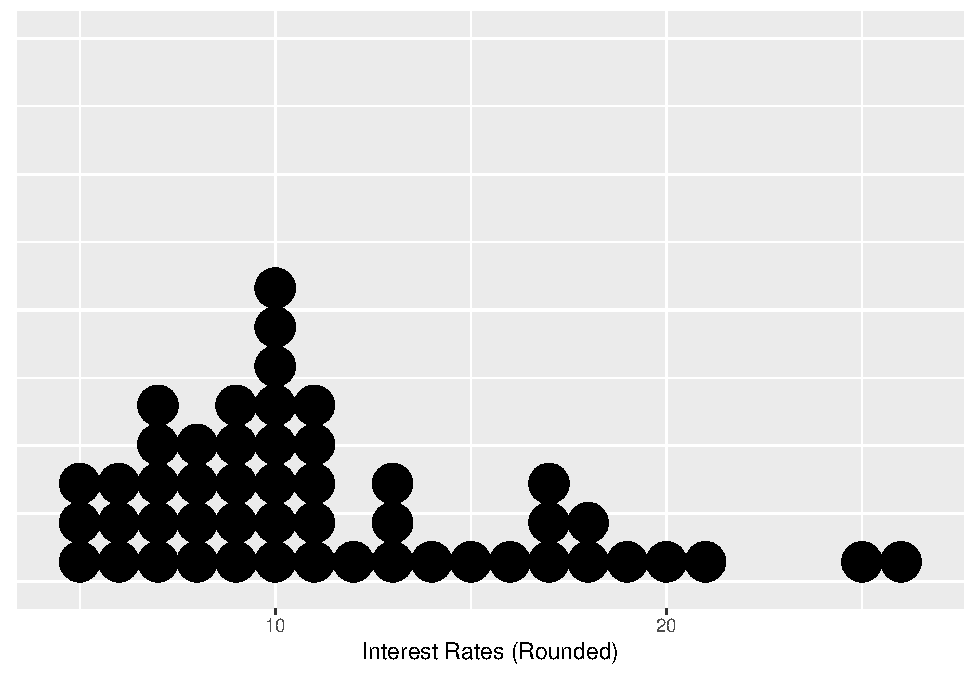
\includegraphics{bookdown-demo_files/figure-latex/dotplot-1.pdf}
\caption{\label{fig:dotplot}Dot Plot for 50 Interest Rates (rounded)}
\end{figure}

Notice there is 1 black dot that corresponds to an interest rate of 20 (presumably in percent), so there is one applicant who has a rounded interest rate of 20 percent. There are 8 black dots that correspond to an interest rate to 10 percent, so there are 8 applicants with a rounded interest rate of 10 percent. So interest rates of 10 percent are much more commonly occurring than interest rate of 20 percent. So we can use the height, or number of dots, to help us glean how often the value of a certain interest rate occurs. Based on this dotplot, interest rates between 5 and 11 percent are common, with higher values being less common.

\emph{Note:} do not get too torn up about the details in the code to produce this dot plot. I have chosen the present the dot plot this way to highlight how we use it, without getting bogged down in the details of how it can be produced. We will not be using dot plots in this class.

\subsection{Histograms}\label{histograms}

It turns out that dot plots are often not useful for large data sets, but they provide the general idea of how other visualizations for larger data sets work. The height of the dots inform us about the frequency of those values occurring.

A visualization that is more commonly used for larger data sets is a \textbf{histogram}. Instead of displaying how common each value of the variable exists, we think of the values as belonging to a \textbf{bin} of values. For example, we can create a bin that contains interest rates between 5 and 7.5 percent, another bin containing interest rates between 7.5 and 10 percent, and so on. A few things to note about histograms:

\begin{itemize}
\item
  By convention, values that lie exactly on the boundary of a bin will belong to the lower bin. For example, an interest rate that is exactly 12.5 percent will belong to the bin between 10 and 12.5 percent, and not the bin between 12.5 to 15 percent.
\item
  Each bin should have the same width. In our example, the width is 2.5.
\end{itemize}

We create this histogram (using the original interest rates) below, per Figure \ref{fig:hist}:

\begin{Shaded}
\begin{Highlighting}[]
\DocumentationTok{\#\#set up sequence to specify the bins}
\NormalTok{s25}\OtherTok{\textless{}{-}}\FunctionTok{seq}\NormalTok{(}\DecValTok{5}\NormalTok{,}\FloatTok{27.5}\NormalTok{,}\FloatTok{2.5}\NormalTok{)}

\FunctionTok{ggplot}\NormalTok{(Data,}\FunctionTok{aes}\NormalTok{(}\AttributeTok{x=}\NormalTok{interest\_rate))}\SpecialCharTok{+}
  \FunctionTok{geom\_histogram}\NormalTok{(}\AttributeTok{breaks=}\NormalTok{s25,}\AttributeTok{fill=}\StringTok{"blue"}\NormalTok{,}\AttributeTok{color=}\StringTok{"orange"}\NormalTok{)}\SpecialCharTok{+}
  \FunctionTok{labs}\NormalTok{(}\AttributeTok{x=}\StringTok{"Interest Rate"}\NormalTok{, }\AttributeTok{title=}\StringTok{"Histogram of Interest Rates"}\NormalTok{)}
\end{Highlighting}
\end{Shaded}

\begin{figure}
\centering
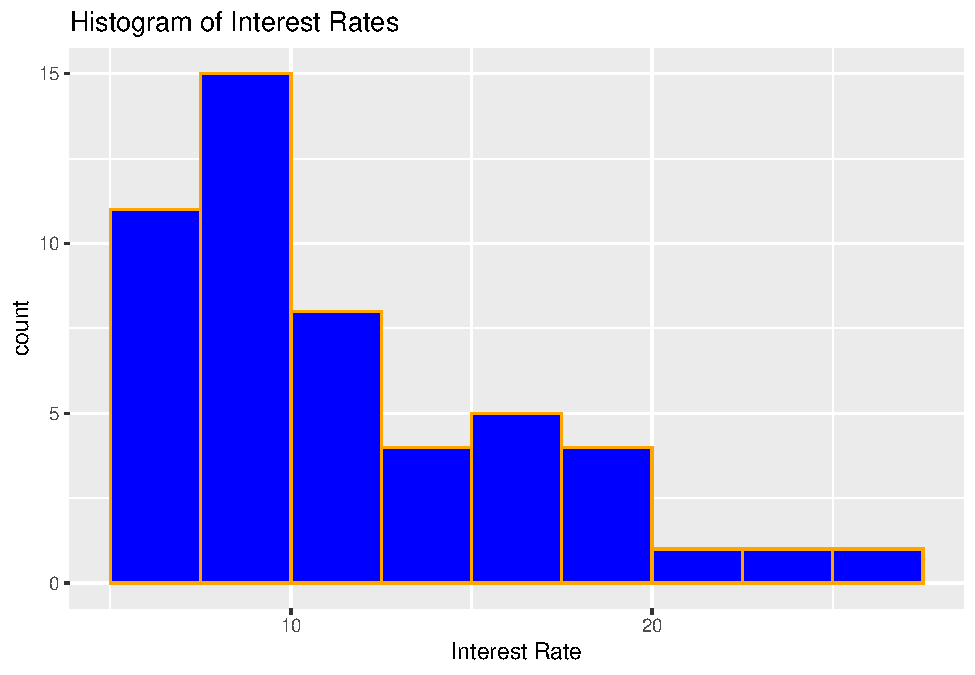
\includegraphics{bookdown-demo_files/figure-latex/hist-1.pdf}
\caption{\label{fig:hist}Historgram for 50 Interest Rates}
\end{figure}

Similar to the dot plot in Figure \ref{fig:dotplot}, the height of the histogram inform us what values are more commonly occurring. We can see from this histogram that interest rates between 5 and 10 percent are common, much more so than loans with interest rates greater than 20 percent. We could say that we have more certainty that a randomly selected loan applicant will have an interest rate between 5 and 10 percent than an interest rate that is greater than 20 percent.

\subsubsection{Shapes of Distribution}\label{shapes-of-distribution}

Histograms can also give us an idea about the \textbf{shape} of the distribution of interest rates. For the histogram in Figure \ref{fig:hist}, most of the loans are less than 15 percent, with only a small number of loans greater than 20 percent. We can say that we have greater certainty that a loan will have an interest rate less than 15 percent. When the data tail off to the right as in our histogram, the shape is said to be \textbf{right-skewed}. When a variable is said to be right-skewed, large values of the variable are much less common than small values of the variable; smaller values are more likely occur.

\begin{itemize}
\item
  If the histogram has the reverse characteristic, i.e.~the data tail off to the left instead, the shape is said to be \textbf{left-skewed}. This implies that small values of the variable are much less common than large values of the variable; larger values are more likely to occur.
\item
  Histograms that tail off similarly in both directions are called \textbf{symmetric}. Large and small values are of the variable are equally likely.
\item
  Histograms that have a peak in the middle, and then tail off on both sides are not only symmetic, but also \textbf{bell-shaped}, or have a \textbf{normal} distribution. Note: it turns out one of the assumptions in linear regression is that the response variable follow a normal distribution. This may seem restrictive, however, we will see in later modules that this assumption is not particularly crucial under some circumstances.
\end{itemize}

\emph{Thought question:} Can you think of real life variables that have symmetric, right-skewed, left-skewed distributions? Feel free to search the internet for examples.

\subsubsection{Considerations with Histograms}\label{considerations-with-histograms}

With our interest rate example, you may have noticed that I made a specific choice on the width of the bins when I created the histograms. It turns out that the width of the bins can impact the shape of the histogram, and potentially, how we interpret the histogram.

Consider creating a histogram with bin width of 0.5, instead of 2.5, per Figure \ref{fig:hist05}:

\begin{Shaded}
\begin{Highlighting}[]
\DocumentationTok{\#\#set up sequence to specify the bins. width now 0.5}
\NormalTok{s05}\OtherTok{\textless{}{-}}\FunctionTok{seq}\NormalTok{(}\DecValTok{5}\NormalTok{,}\FloatTok{27.5}\NormalTok{,}\FloatTok{0.5}\NormalTok{)}

\FunctionTok{ggplot}\NormalTok{(Data,}\FunctionTok{aes}\NormalTok{(}\AttributeTok{x=}\NormalTok{interest\_rate))}\SpecialCharTok{+}
  \FunctionTok{geom\_histogram}\NormalTok{(}\AttributeTok{breaks=}\NormalTok{s05,}\AttributeTok{fill=}\StringTok{"blue"}\NormalTok{,}\AttributeTok{color=}\StringTok{"orange"}\NormalTok{)}\SpecialCharTok{+}
  \FunctionTok{labs}\NormalTok{(}\AttributeTok{x=}\StringTok{"Interest Rate"}\NormalTok{, }\AttributeTok{title=}\StringTok{"Histogram of Interest Rates"}\NormalTok{)}
\end{Highlighting}
\end{Shaded}

\begin{figure}
\centering
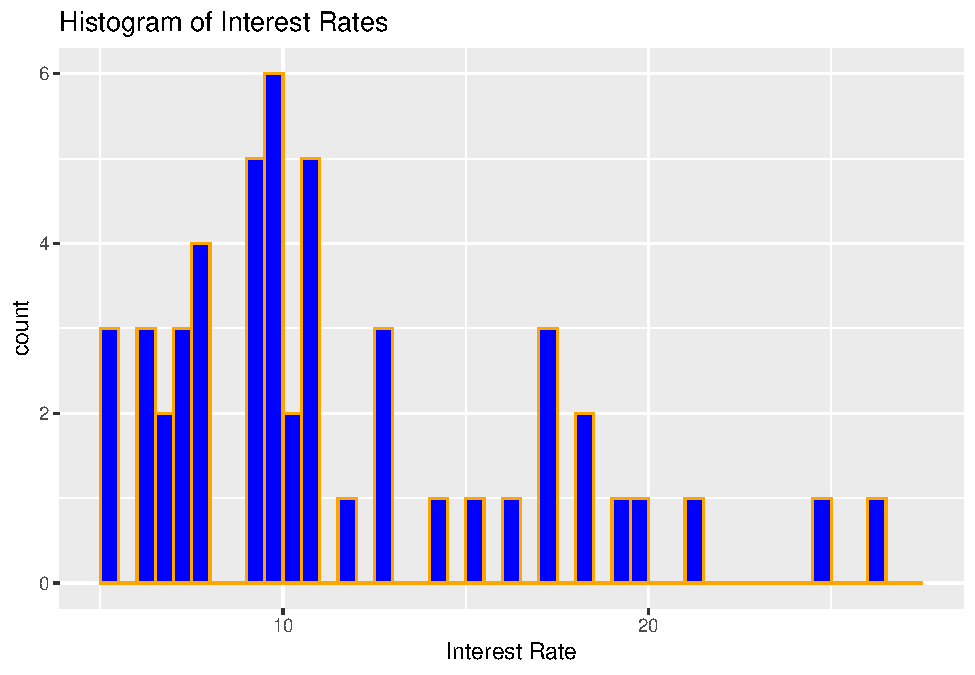
\includegraphics{bookdown-demo_files/figure-latex/hist05-1.pdf}
\caption{\label{fig:hist05}Historgram for 50 Interest Rates, with Bin Width 0.5}
\end{figure}

Comparing Figure \ref{fig:hist05} with Figure \ref{fig:hist}, note the following:

\begin{itemize}
\item
  Visually, the histogram looks more jagged with smaller bin width, whereas the histogram looks smoother with a larger bin width.
\item
  Smaller bin widths may be preferred if we need information about smaller ranges of interest rates. However, it can be difficult to write about general trends.
\item
  Larger bin widths may be more useful if we are trying to look for more general trends in the interest rates.
\end{itemize}

\emph{Thought question}: What happens if we create a histogram with a bin width that is too large?

\subsection{Density Plots}\label{densplots}

Another visualization for a quantitative variable is a \textbf{density plot}. A density plot can be viewed as a smoothed version of the histogram. We can use the heights to inform us about what values are more common. We create a density plot for the interest rates in Figure \ref{fig:dens}:

\begin{Shaded}
\begin{Highlighting}[]
\DocumentationTok{\#\#density plot}
\FunctionTok{plot}\NormalTok{(}\FunctionTok{density}\NormalTok{(Data}\SpecialCharTok{$}\NormalTok{interest\_rate), }\AttributeTok{main=}\StringTok{"Density Plot of Interest Rates"}\NormalTok{)}
\end{Highlighting}
\end{Shaded}

\begin{figure}
\centering
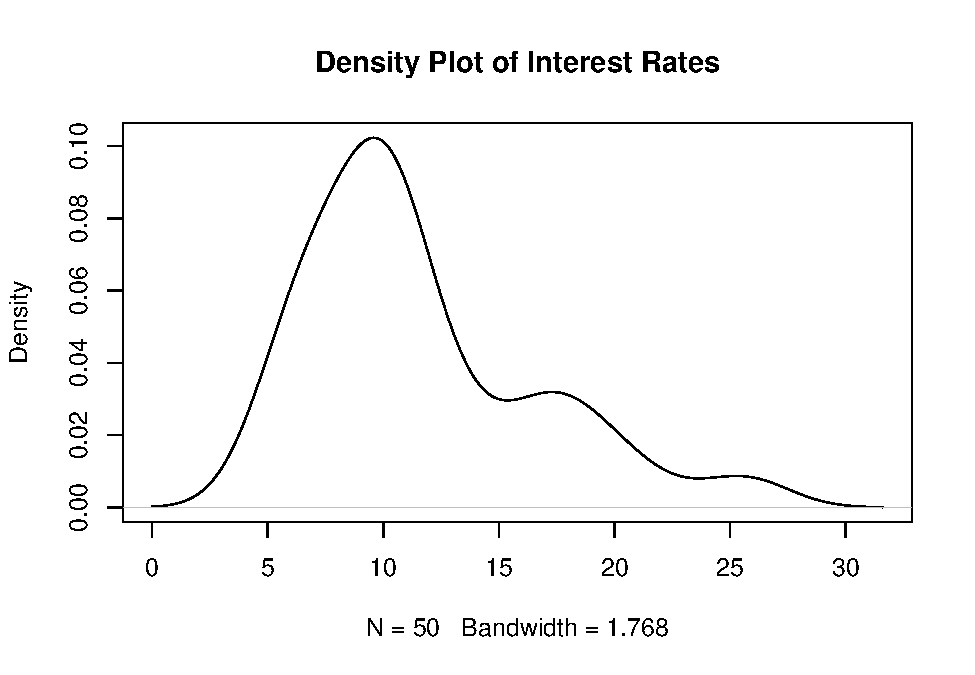
\includegraphics{bookdown-demo_files/figure-latex/dens-1.pdf}
\caption{\label{fig:dens}Density Plot for 50 Interest Rates}
\end{figure}

Based on Figure \ref{fig:dens}, we see that low interest rates (between 5 and 12.5 percent) are much more common and high interest rates (higher than 20 percent). A few things to note about interpreting density plots:

\begin{itemize}
\tightlist
\item
  The area under the density plot is always equals to 1.
\item
  To find the proportion of interest rates that are between two values, for example between 10 and 15 percent, we would integrate this density plot over this range, i.e.~\(\int_{10}^{15} f(x) dx\), where \(f(x)\) is a mathematical equation that describes the density plot. We will learn about this equation in more detail in a later module.
\item
  The values on the vertical axis do not equal to probabilities (a common misconception).
\end{itemize}

The density plot is found using a method called kernel density estimation (KDE). We will over details about KDE in Section \ref{KDE} as we need to cover quite a bit of material before doing so.

\subsubsection{Considerations with Density Plots}\label{considerations-with-density-plots}

Similar to bins and histograms, density plots are affected by the \textbf{bandwidth}. Larger bandwidths lead to smoother density plots, while smaller bandwidths lead to more jagged density plots. We create a density plot that uses a bandwidth that is twice the default in Figure \ref{fig:dens2} below:

\begin{Shaded}
\begin{Highlighting}[]
\FunctionTok{plot}\NormalTok{(}\FunctionTok{density}\NormalTok{(Data}\SpecialCharTok{$}\NormalTok{interest\_rate, }\AttributeTok{adjust=}\DecValTok{2}\NormalTok{), }\AttributeTok{main=}\StringTok{"Density Plot of Interest Rates, with Bandwidth Twice the Default"}\NormalTok{)}
\end{Highlighting}
\end{Shaded}

\begin{figure}
\centering
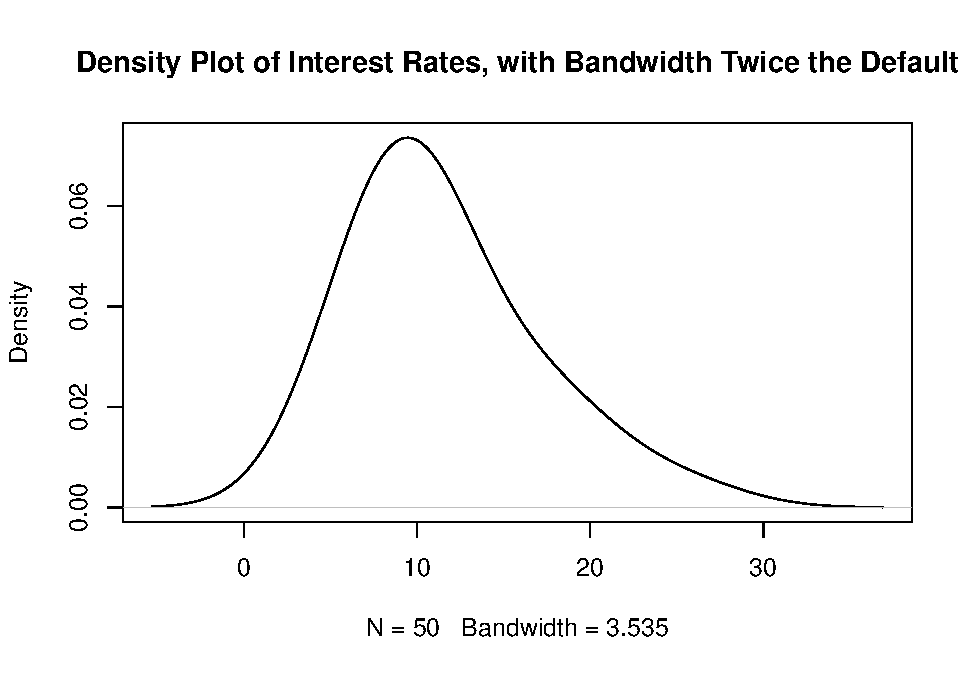
\includegraphics{bookdown-demo_files/figure-latex/dens2-1.pdf}
\caption{\label{fig:dens2}Density Plot for 50 Interest Rates with Larger Bandwidth}
\end{figure}

Notice in Figure \ref{fig:dens2} that the little peak for interest rates between 15 and 20 (which existed in Figures \ref{fig:dens} and also \ref{fig:hist}) no longer exists. Using bandwidths that are too large can smooth out some of these peaks.

\emph{Thought question}: How are bin widths for histograms and bandwidths for density plots related?

\section{Ordered Statistics}\label{ordered-statistics}

The idea behind ordered statistics is pretty self-explanatory: take your numerical variable, and order the values from smallest to largest. Going back to our example of the interest rates from 50 loan applicants, let \(X\) denote the interest rate. Then \(x_{(1)}\) will denote the interest rate that is the smallest, \(x_{(2)}\) denotes the second smallest interest rate, and \(x_{(50)}\) denotes the largest interest rate in our sample of 50.

\subsection{Quantiles}\label{quantiles}

\textbf{Quantiles} partition the range of numerical data into continuous intervals (groups) with (nearly) equal proportions. Common quantiles have their own names:

\begin{itemize}
\tightlist
\item
  Quartiles: 4 groups
\item
  Percentiles: 100 groups
\end{itemize}

We will go over quartiles in more detail.

\subsubsection{Quartiles}\label{quart}

Quartiles divide the data into 4 groups, and each group has (nearly) equal number of observations. So there will be three quartiles, denoted by \(Q_1, Q_2, Q_3\).

\begin{itemize}
\tightlist
\item
  The first group will have values between negative infinity and \(Q_1\).
\item
  The second group will have values between negative \(Q_1\) and \(Q_2\).
\item
  The third group will have values between negative \(Q_2\) and \(Q_3\).
\item
  The fourth group will have values between negative \(Q_3\) and infinity.
\end{itemize}

\(Q_2\), sometimes called the second quartile, is the easiest value to find. It is also called the \textbf{median} of the data. Going back to our interest rates from the 50 loan applicants. Using our ordered statistics, the median is the middle observation. Since we have an even number of observations, we have two middle observations, \(x_{(25)}\) and \(x_{(26)}\). In this situation, the median will be the average of these two middle observations. Using R, we find the median to be:

\begin{Shaded}
\begin{Highlighting}[]
\FunctionTok{median}\NormalTok{(Data}\SpecialCharTok{$}\NormalTok{interest\_rate)}
\end{Highlighting}
\end{Shaded}

\begin{verbatim}
## [1] 9.93
\end{verbatim}

So roughly half the interest rates are less than 9.93 percent, and roughly half the interest rates are greater than 9.93 percent. You might also recognize another term for the median: the 50th percentile, as 50 percent of the interest rates are less than 9.93.

To find the middle observation(s) based on a sample of size \(n\):

\begin{itemize}
\tightlist
\item
  If \(n\) is even, the 2 middle observations will be position \(\frac{n}{2}\) and \(\frac{n}{2} + 1\) in the ordered statistics.
\item
  If \(n\) is odd, the middle observation will be position \(\frac{n}{2} + 0.5\) in the ordered statistics.
\end{itemize}

\(Q_1\) and \(Q_3\) (also called the first and third quartiles) are found together, after finding \(Q_2\). Note that \(Q_2\) divides the data into two groups. Using our interest rates example, one group contains \(x_{(1)}, \cdots, x_{(25)}\), and another group contains \(x_{(26)}, \cdots, x_{(50)}\). \(Q_1\) is the median of the first group, and \(Q_3\) is the median of the second group. So for our 50 loan applicants:

\begin{itemize}
\tightlist
\item
  \(Q_1\) is \(x_{(13)}\), and
\item
  \(Q_3\) is \(x_{(38)}\).
\end{itemize}

To find these values in R, we could type:

\begin{Shaded}
\begin{Highlighting}[]
\FunctionTok{quantile}\NormalTok{(Data}\SpecialCharTok{$}\NormalTok{interest\_rate, }\AttributeTok{prob=}\FunctionTok{c}\NormalTok{(}\FloatTok{0.25}\NormalTok{,}\FloatTok{0.75}\NormalTok{), }\AttributeTok{type =} \DecValTok{1}\NormalTok{)}
\end{Highlighting}
\end{Shaded}

\begin{verbatim}
##   25%   75% 
##  7.96 14.08
\end{verbatim}

So \(Q_1\) is 7.96 percent, and \(Q_3\) is 14.08 percent. It turns out that \(Q_1\) is also the 25th percentile, and \(Q_3\) is also the 75th percentile, by definition.

Remember we wrote the following earlier:

\begin{itemize}
\tightlist
\item
  The first group will have values between negative infinity and \(Q_1\). So about a quarter of observations are have interest rates less than 7.96 percent.
\item
  The second group will have values between negative \(Q_1\) and \(Q_2\). So about a quarter of observations have interest rates between 7.96 and 9.93 percent.
\item
  The third group will have values between negative \(Q_2\) and \(Q_3\). So about a quarter of observations have interest rates between 9.93 and 14.08 percent.
\item
  The fourth group will have values between negative \(Q_3\) and infinity. So about a quarter of observations have interest rates above 14.08 percent.
\end{itemize}

Note: you may notice that we used \texttt{type\ =\ 1} inside the \texttt{quantile()} function. Using \texttt{type\ =\ 1} gives the values of the first and third quartiles that are based on the method that was just described. There are actually several ways to find quantiles, which may result in slightly differing values, although they all generally meet the definition that \(Q_1\) is the 25th percentile, and \(Q_3\) is the 75th percentile.

\subsubsection{Percentiles}\label{percentiles}

Another common quantile is the percentile. In general the \textbf{k-th percentile} is the value of the data point below which \(k\) percent of observations are found. So in our earlier example, we said that \(Q_3\) of the interest rates is 14.08 percent, and this is also the 75th percentile. So 75 percent of interest rates are less than 14.08 percent.

\subsection{Box Plots}\label{box-plots}

Another visualization used to summarize quantitative data is the box plot. A \textbf{box plot} summarizes the 5-number summary. The 5 numbers are the minimum, \(Q_1, Q_2, Q_3\), and the maximum. Using our interest rate data, the box plot is shown in Figure \ref{fig:boxplot}:

\begin{Shaded}
\begin{Highlighting}[]
\DocumentationTok{\#\#box plot}
\FunctionTok{ggplot}\NormalTok{(Data,}\FunctionTok{aes}\NormalTok{(}\AttributeTok{y=}\NormalTok{interest\_rate))}\SpecialCharTok{+}
  \FunctionTok{geom\_boxplot}\NormalTok{()}\SpecialCharTok{+}
  \FunctionTok{labs}\NormalTok{(}\AttributeTok{y=}\StringTok{"Interest Rate"}\NormalTok{, }\AttributeTok{title=}\StringTok{"Box Plot of Interest Rates"}\NormalTok{)}
\end{Highlighting}
\end{Shaded}

\begin{figure}
\centering
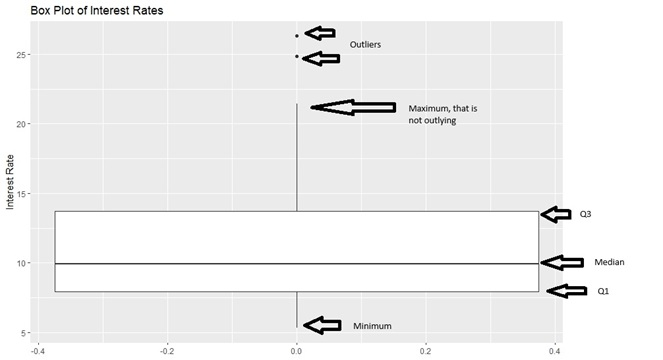
\includegraphics{images/01-boxplot.jpeg}
\caption{\label{fig:boxplot}Box Plot of Interest Rates}
\end{figure}

Some people call a box plot a box and whisker plot.

\begin{itemize}
\tightlist
\item
  The boundaries of the box represent \(Q_1\) and \(Q_3\).
\item
  The thick line in the box represents the median.
\item
  The two whiskers on either side of the box extend to the minimum and maximum, if outliers do not exist. If outliers exist, the whiskers extend to the minimum and maximum values that are not outliers.
\end{itemize}

Generally, when we have one quantitative variable, an outlier is an observation whose numerical value is far away from the rest of the data. In other words, it is a lot smaller or larger relative to the rest of the data.

So for our 50 loans, there are two loan applicants with interest rates around 25 percent that are flagged as being a lot larger than the rest of the loans, which is reasonable since most of the loans are a lot smaller than 20 percent.

We will not go over the details of how outliers are determined in box plots. If you are interested, you can read Chapter 2.1.5 from \href{https://www.openintro.org/book/os/}{OpenIntro Statistics (Diez, Ceytinka-Rundel, Barr)}. Generally, when we are working with one variable, outliers are observations which are a lot larger or smaller than the rest of the observations.

Notice how much further large values (\(Q_3\) and maximum) are from the median, compared to the distance of the small values (\(Q_1\) and minimum) from the median. This indicates that the distribution of interest rates are right-skewed. Compare the boxplot of the interest rates in Figure \ref{fig:boxplot} with its corresponding histogram (Figure \ref{fig:hist}) and density plot (Figure \ref{fig:dens}).

\emph{Thought question}: can you sketch a box plot that represents a variable that is left-skewed? How about a variable that is symmetric?

\subsection{Empirical Cumulative Distribution Function}\label{ecdf}

From the previous sections, we can see how we could use histograms, density plots, and box plots to inform us about what proportion of observations take certain values, and the values of the data that correspond to certain percentiles. However, we are limited to quartiles and not any percentile when using box plots, and we need to find areas under the density plot (using integration, not a trivial task), or add up frequencies on a histogram (can be time consuming).

A plot that can easily give us values of the variable that correspond to percentiles is the \textbf{empirical cumulative distribution function (ECDF)} plot.

Let \(X\) denote a random variable, and we have observed \(n\) observations of \(X\) denoted by \(x_1, \cdots, x_n\). Let \(x_{(1)}, \cdots x_{(n)}\) denote the ordered statstics of the \(n\) observations. The ECDF, denoted by \(\hat{F}_n(x)\) is the proportion of sample observations less than or equal to the value \(x\) of the random variable. Mathematically, the ECDF is:

\[
 \hat{F}_n(x) = 
  \begin{cases} 
   0, & \text{for } x < x_{(1)} \\
   \frac{k}{n},       & \text{for } x_{(k)} \leq x < x_{(k+1)}, k = 1, \cdots, n-1\\
   1, & \text{for } x \geq x_{(n)}.
  \end{cases}
\]
We shall use a simple toy example to illustrate how an ECDF is constructed. Suppose we ask 5 people how many times to go to the gym (at least 20 minutes) in a typical work week. The answers are: 3, 0, 1, 5, 3. The random variable \(X\) is how many times a person goes to the gym for at least 20 minutes, and the ordered statistics are \(x_{(1)} = 0, x_{(2)} = 1, x_{(3)} = 3, x_{(4)} = 3, x_{(5)} = 5\). Using the mathematical definition for the ECDF, we have:

\begin{itemize}
\tightlist
\item
  \(\hat{F}_n(x) = 0\) for \(x < x_{(1)} = 0\).
\item
  \(\hat{F}_n(x) = \frac{1}{5}\) for \(0 \leq x < x_{(2)} = 1\).
\item
  \(\hat{F}_n(x) = \frac{2}{5}\) for \(1 \leq x < x_{(3)} = 3\).
\item
  \(\hat{F}_n(x) = \frac{4}{5}\) for \(3 \leq x < x_{(5)} = 5\). This value is special for this example since we have two observations where \(x=3\).
\item
  \(\hat{F}_n(x) = 1\) for \(x \geq 5\).
\end{itemize}

The corresponding ECDF plot is shown in Figure \ref{fig:ecdf}:

\begin{Shaded}
\begin{Highlighting}[]
\DocumentationTok{\#\#toy data}
\NormalTok{y}\OtherTok{\textless{}{-}}\FunctionTok{c}\NormalTok{(}\DecValTok{3}\NormalTok{, }\DecValTok{0}\NormalTok{, }\DecValTok{1}\NormalTok{, }\DecValTok{5}\NormalTok{, }\DecValTok{3}\NormalTok{)}
\DocumentationTok{\#\#ECDF plot}
\FunctionTok{plot}\NormalTok{(}\FunctionTok{ecdf}\NormalTok{(y), }\AttributeTok{main =} \StringTok{"ECDF for Toy Example"}\NormalTok{)}
\end{Highlighting}
\end{Shaded}

\begin{figure}
\centering
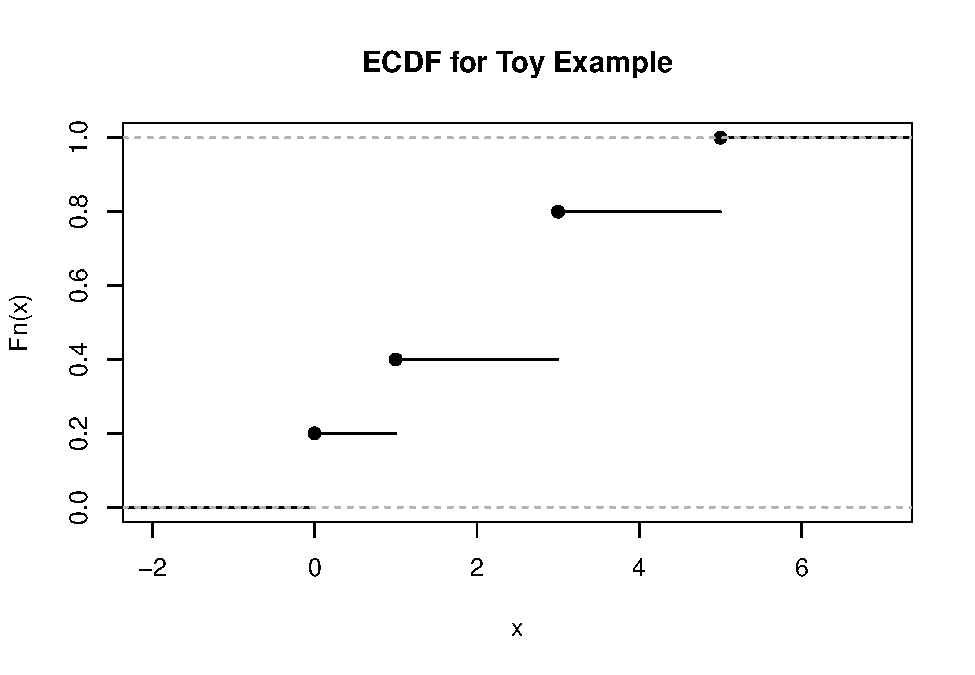
\includegraphics{bookdown-demo_files/figure-latex/ecdf-1.pdf}
\caption{\label{fig:ecdf}ECDF Plot for Toy Example}
\end{figure}

We can easily find percentiles from this plot, for example, the 40th percentile is equal to 1, going to the gym once a week. About 20 percent of observations go to the gym less than 1 time a week. The video below explains the construction of the ECDF:

Next, we create the ECDF plot for the interest rates from the 50 loan applicants.

\begin{Shaded}
\begin{Highlighting}[]
\FunctionTok{plot}\NormalTok{(}\FunctionTok{ecdf}\NormalTok{(Data}\SpecialCharTok{$}\NormalTok{interest\_rate), }\AttributeTok{main =} \StringTok{"ECDF Plot of Interest Rates"}\NormalTok{)}
\FunctionTok{abline}\NormalTok{(}\AttributeTok{h=}\FloatTok{0.8}\NormalTok{)}
\end{Highlighting}
\end{Shaded}

\begin{figure}
\centering
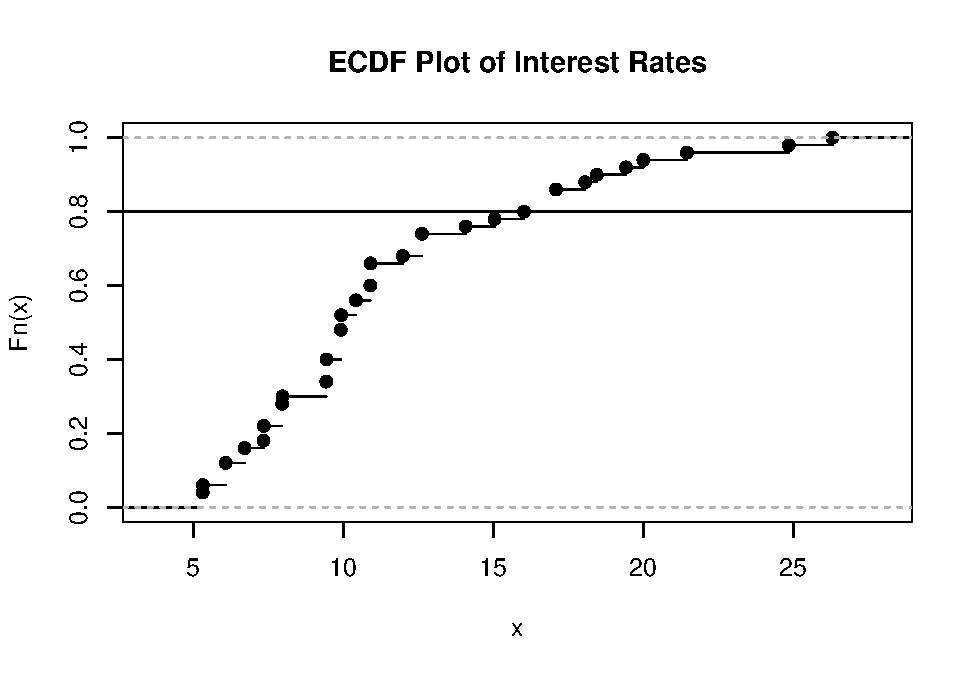
\includegraphics{bookdown-demo_files/figure-latex/ecdfreal-1.pdf}
\caption{\label{fig:ecdfreal}ECDF Plot of Interest Rates}
\end{figure}

I overlaid a horizontal line for the 80th percentile, so we can read on the horizontal axis that this corresponds to an interest rate of about 17 percent. So about 80 percent of loan applicants have an interest rate less than 17 percent.

\emph{Thought question}: try using the histogram and density plot for the interest rates (Figures \ref{fig:hist} and \ref{fig:dens}) to find the interest rate that corresponds to the 80th percentile. Was this easy to perform?

\section{Measures of Centrality}\label{measures-of-centrality}

So far, we have used visualizations to summarize the shape of the distribution of a quantitative variable. Next, we look at common measures of centrality. Loosely speaking, measures of centrality are measures that describe the average or typical value of a quantitative variable. The common measures of centrality are the mean, median, and mode.

\subsection{Mean}\label{mean}

The sample \textbf{mean} is simply the average value of the variable in our sample. The sample mean for a random variable \(X\) is denoted by \(\bar{x}\), and is found by:

\begin{equation} 
\bar{x} = \frac{\sum_{i=1}^n x_i}{n}.
\label{eq:mean}
\end{equation}

So, for our toy example of the 5 people and how often they go to the gym in a week, their sample mean is \(\bar{x} = \frac{3+0+1+5+3}{5} = 2.4\).

\subsection{Median}\label{median}

We went over how to find the median in section \ref{quart}. The \textbf{median} is the value of the middle observation in ordered statistics. It is also called \(Q_2\), the second quartile, and the 50th percentile, so approximately 50 percent of observations have values smaller than the median.

So, for our toy example of the 5 people and how often they go to the gym in a week, their sample median is \(x_{(3)} = 3\). So about 50 percent of people went to gym less than 3 times in a week.

\subsection{Mode}\label{mode}

Another measure is the mode. Mathematically speaking, the \textbf{mode} is the most commonly occurring value in the data. So for our toy example, the mode is 3, since 3 occurs twice and occurs the most often in our data.

\subsection{Considerations}\label{considerations}

A few things to consider when using these measures of centrality:

\begin{itemize}
\item
  The mean is a measure that most people are comfortable with, however, caution needs to be used if the variable is skewed, as extreme outliers and drastically alter the value of the mean. Using our toy example with the gym, suppose the person who visits the gym the most visits 50 times, instead of 5. The numerical value of the sample mean explodes, and does not give a good representation of the central value of how many visits to the gym a person makes in a week. The mean is fine if the variable is symmetric.
\item
  The median is a measure that is recommended for skewed distributions, since the order associated with ordered statistics is not influenced by extreme outliers. Using the gym example, in the previous bullet point, the median is unaffected.
\item
  The mean being larger than the median is an indication that the distribution is right-skewed. Using our interest rate example, we have:
\end{itemize}

\begin{Shaded}
\begin{Highlighting}[]
\FunctionTok{mean}\NormalTok{(Data}\SpecialCharTok{$}\NormalTok{interest\_rate)}
\end{Highlighting}
\end{Shaded}

\begin{verbatim}
## [1] 11.5672
\end{verbatim}

\begin{Shaded}
\begin{Highlighting}[]
\FunctionTok{median}\NormalTok{(Data}\SpecialCharTok{$}\NormalTok{interest\_rate)}
\end{Highlighting}
\end{Shaded}

\begin{verbatim}
## [1] 9.93
\end{verbatim}

which is consistent with the right skew we saw in the histogram and density plot in Figures \ref{fig:hist} and \ref{fig:dens}. Conversely, a left-skewed distribution usually has a mean that is smaller than the median. A symmetric distribution typically has similar values for the mean and median.

\begin{itemize}
\item
  The mean is considered a \textbf{sensitive} measure, since its numerical value can be drastically affected by outliers. The median is considered a \textbf{robust} measure, since its numerical value is more resistant and is less affected by outliers.
\item
  The mathematical definition of mode can be difficult to use for variables that are continuous, since it is likely that there are no observations that have the same value when the variable is continuous. In this instance, the mode typically refers to the bin in the histogram that has is the tallest. So, using the histogram in Figure \ref{fig:hist} for the interest rates, the mode is between 7.5 to 10 percent.
\end{itemize}

\section{Measures of Spread}\label{measures-of-spread}

In the previous sections, we learned about summarizing features a quantitative variable, by using visualizations to summarize its shape, and by using some measures of centrality that describe the average or typical values of the variable. One more feature we can summarize is the spread, associated with the values of a quantitative variable. Measures of spread are considered a way to measure uncertainty. Data that have larger spread have more uncertainty.

\subsection{Variance and Standard Deviation}\label{variance-and-standard-deviation}

One measure of spread is the variance. The sample \textbf{variance} for a random variable \(X\) is denoted by \(s^2\), or sometimes \(s_x^2\), and is found by:

\begin{equation} 
s^2 = \frac{\sum_{i=1}^n (x_i-\bar{x})^2}{n-1}.
\label{eq:variance}
\end{equation}

The variance can be interpreted as the approximate average squared distance of the observations from the mean. The formula in equation \eqref{eq:variance} may look a bit complicated, but let us use the toy example where we asked 5 people how often they go to the gym in a workweek. The answers are: 3, 0, 1, 5, 3, and we had earlier found the sample mean to be \(\bar{x} = 2.4\). To calculate the sample variance:

\[
\begin{split}
s^2 &= \frac{\sum_{i=1}^n (x_i-\bar{x})^2}{n-1}\\
 &= \frac{(3-2.4)^2 + (0-2.4)^2 + (1-2.4)^2 + (5-2.4)^2 + (3-2.4)^2}{5-1} \\
&= 3.8 
\end{split}
\]

Notice what we did in the numerator of equation \eqref{eq:variance}: we take the difference between each observed value from the sample mean, square these differences, then add up the squared differences. We then divide by \(n-1\), rather than \(n\), hence the sample variance being the approximate averaged squared distance of the observations from the mean. There is some nuance in the mathematics as to why we divide by \(n-1\) instead of \(n\), and may not be intuitive as to why we do so. It turns out dividing by \(n-1\) makes the sample variance an unbiased estimator of the true variance in the population (denoted by \(\sigma^2\)) and is more reliable than if we had divided by \(n\). We will go over this in more detail in a later module after covering a few additional concepts.

The video below explains the calculation of the sample variance:

Larger values of the sample variance indicate that the observations are generally further away from the sample mean, indicating larger spread, and a higher degree of uncertainty about future values.

\emph{Thought question}: What does it mean if the sample variance of a set of observations is 0? Why does this indicate their there is little (or no) uncertainty about the set of observations?

Another related measure is the sample \textbf{standard deviation}, which is the square root of the sample variance. Similar to the variance, larger values indicated more spread in the data.

\subsection{Interquartile Range}\label{interquartile-range}

Another measure of spread is the \textbf{interquartile range (IQR)}, and it is the difference between the third and first queartiles,

\begin{equation} 
IQR = Q_3 - Q_1.
\label{eq:IQR}
\end{equation}

The IQR is considered a robust measure of spread, while the sample variance and standard deviations are considered to be sensitive.

\chapter{Probability}\label{probability}

This module is based on Introduction to Probability (Blitzstein, Hwang), Chapters 1 and 2. You can access the book for free at \url{https://stat110.hsites.harvard.edu/} (and then click on Book). Please note that I cover additional topics, and skip certain topics from the book. You may skip: Sections 1.4, 1.5, Theorem 1.6.3, Examples 1.6.4, 2.4.5, 2.5.12, 2.7.3 from the book.

\section{Introduction to Probability}\label{introduction-to-probability}

A way of quantifying uncertainty is through probability. Think about these statements: ``I am 100\% certain that it will rain in the next hour'' and ``I am 50\% certain that it will rain in the next hour''. The percentages are used to reflect the degree of certainty about the event happening. The first statement reflects certainty; the second reflects uncertainty as the statement implies the belief that it is equally likely that it will rain or not. In this module, we will learn about the basic concepts about probability.

\subsection{Why Study Probability?}\label{why-study-probability}

The book (Section 1.1) lists 10 different applications of probability, and there are many more applications. I will go as far as to say that anything that deals with data will also deal with probability.

\subsection{Frequentiest and Bayesian View of Probability}\label{frequentiest-and-bayesian-view-of-probability}

There are a couple of viewpoints on how to interpret probability: \textbf{frequentist} and \textbf{Bayesian}. Consider the statement that ``if we flip a fair coin, the coin has a 50\% chance of landing heads''.

\begin{itemize}
\item
  The frequentist viewpoint views probability as the relative frequency associated with an event that is repeated for an infinite number of times. It will interpret the 50\% probability as: if we were to flip the coin many many times, 50\% of these times will result in the coin landing heads.
\item
  The Bayesian viewpoint views probability as a measure of belief, or certainty, that an event will happen. It will interpret the 50\% probability as: heads and tails are equally likely to occur with a coin flip.
\end{itemize}

In this coin flip example, both interpretations are reasonable. However, in some instances, the frequentist interpretation may not be as interpretable if we cannot repeat the event many times. For example, the earlier statement about rain: ``I am 50\% certain that it will rain in the next hour''. Whether it will rain or not in the next hour is not a repeatable event, so the frequentist interpretation makes less sense here.

\section{Key Concepts in Probability}\label{key-concepts-in-probability}

In this section, we will cover the basic terminology and foundational ideas in probability.

\subsection{Sample Space}\label{sample-space}

The \textbf{sample space} of an experiment, denoted by \(S\), is the set of all possible outcomes of an experiment.

For the rest of this module, we will use the following as an example: consider a standard deck of 52 cards, and we draw one card at random. What is the card drawn? The sample space for this experiment can be viewed as a list of all 52 cards, per Figure \ref{fig:cards} below.

\begin{figure}
\centering
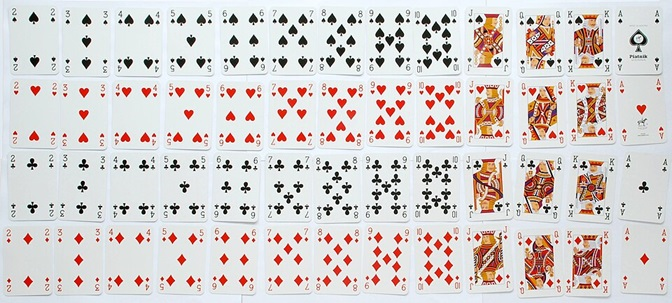
\includegraphics{images/02-cards.jpg}
\caption{\label{fig:cards}Sample Space of Drawing One Card from Standard Deck. Picture from \url{https://en.wikipedia.org/wiki/Standard_52-card_deck}}
\end{figure}

While the definition of sample space may appear elementary, writing out the sample space is almost always the first step in performing any probability calculations.

\subsection{Event}\label{event}

An \textbf{event} is a subset of the sample space, and is usually denoted by an upper case letter. For example, let \(A\) denote the event that I draw a card with a black suit (spades or clubs), and let \(B\) denote the event I draw a picture card (Jack, Queen, or King). Events \(A\) and \(B\) are each shown in Figures Figure \ref{fig:cardsA} and Figure \ref{fig:cardsB} below.

\begin{figure}
\centering
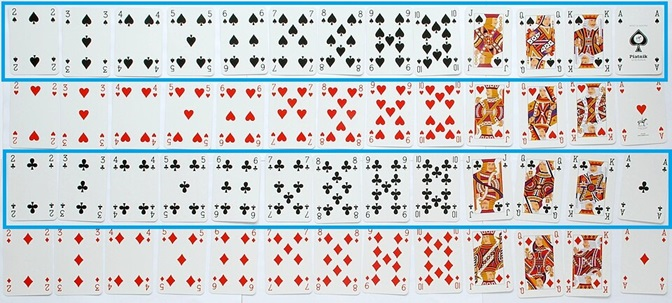
\includegraphics{images/02-cardsA.jpg}
\caption{\label{fig:cardsA}Event \(A\) (in Blue)}
\end{figure}

\begin{figure}
\centering
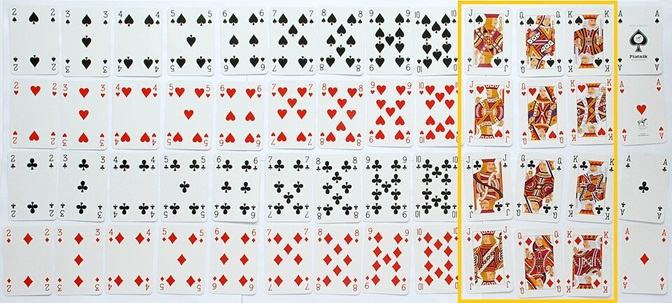
\includegraphics{images/02-cardsB.jpg}
\caption{\label{fig:cardsB}Event \(B\) (in gold)}
\end{figure}

The sample space of the experiment can be finite or infinite. In our card example, our sample space is finite since we can actually write out all possible outcomes. If the number of possible outcomes is infinite (i.e.~we cannot write out the entire list of all possible outcomes), the sample space is infinite.

We assign a probability to each event. The probability of event \(A\) happening is \(P(A)\). \textbf{If each outcome of a sample space is equally likely and we have a finite sample space, the probability of the event is the number of outcomes belonging to the event divided by the number of outcomes in the sample space.} Using our card example, \(P(A) = \frac{26}{52} = \frac{1}{2}\) and \(P(B) = \frac{12}{52} = \frac{3}{13}\).

\subsection{Complements}\label{complements}

The \textbf{complement} of an event is the set of all outcomes that do not belong to the event. For example, the complement of \(A\), denoted by \(A^c\), will be drawing a card with a red suit (hearts or diamonds). One way to think about complements is that the complement of an event is the event not happening. Loking at Figure \ref{fig:cardsA}, this will be the cards that are not outlined in blue. In this example, \(P(A^c) = \frac{26}{52} = \frac{1}{2}\).

\emph{Thought question}: What is the probability of drawing a non picture card?

From these examples, you might realize the probability associated with the complement of an event can be found by subtracting the probability of the event from 1, i.e.

\begin{equation} 
P(A^c) = 1 - P(A).
\label{eq:comp}
\end{equation}

Sometimes, the calculation for the probability of the complement of an event is much less tedious than the probability of the event. In such an instance, equation \eqref{eq:comp} will be useful.

\subsection{Unions}\label{unions}

The \textbf{union} of events is when \textbf{at least one} of the events happen. For example, the union of events \(A\) and \(B\), denoted by \(A \cup B\), is the event that the card drawn is either a black suit, or a picture card, or both a black suit and a picture card. This is reflected in Figure \ref{fig:cardsAB}.

\begin{figure}
\centering
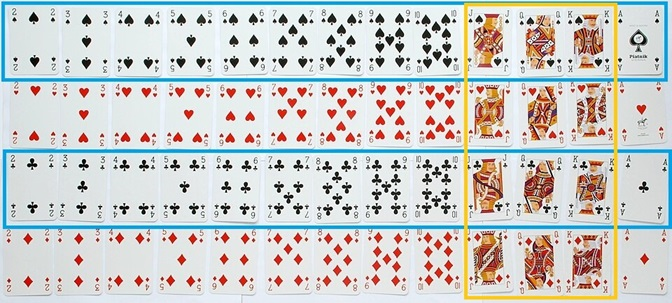
\includegraphics{images/02-cardsAB.jpg}
\caption{\label{fig:cardsAB}Union of A, B (in blue or gold, or both blue and gold)}
\end{figure}

To find \(P(A \cup B)\), we can refer to Figure \ref{fig:cardsAB} and just count the number of outcomes to belong to either event \(A\) (is black suit) or event \(B\) (is picture card), and find this is \(\frac{32}{52}\).

The union of \(A\) and \(B\) can be viewed as the event where either event \(A\) or \(B\) (or both) happens.

\subsection{Intersections}\label{intersections}

The \textbf{intersection} of events is when \textbf{all} of the events happen. Using our example, the intersection of events \(A\) and \(B\) is denoted by \(A \cap B\), is the event that the card drawn is both a black suit and a picture card. Using Figure \ref{fig:cardsAB}, the outcomes belonging to \(A \cap B\) are the cards that are outlined in blue and gold. This probability is \(P(A \cap B) = \frac{6}{52}\).

\subsection{Addition Rule}\label{addition-rule}

A common mistake that can be made in calculating \(P(A \cup B)\) is to just add up the probabilities of each individual event, so the mistake will say this probability is \(\frac{26}{52} + \frac{12}{52} = \frac{38}{52}\). The problem with this approach is that the outcomes that belong to both events (black picture cards) get counted twice, when we only want to count them once. This leads to the following formula for calculating probabilities involving unions of two events, and is sometimes called the \textbf{addition rule} in probability:

\begin{equation} 
P(A \cup B) = P(A) + P(B) - P(A \cap B).
\label{eq:union}
\end{equation}

Using equation \eqref{eq:union}, \(P(A \cup B) = \frac{26}{52} + \frac{12}{52} - \frac{6}{32} = \frac{32}{52}\).

The video below explains the addition rule with this example in a bit more detail:

\subsection{Disjoint or Mutually Exclusive Events}\label{disjoint-or-mutually-exclusive-events}

The previous discussion leads to the idea of \textbf{disjoint}, or \textbf{mutually exclusive} events. Events are disjoint if they cannot happen simultaneously. In our card example, events \(A\) and \(B\) are not disjoint, since \(A\) and \(B\) can happen simultaneously, since a card that is drawn can be both black and a picture card, e.g.~we draw a king of spades.

Using Figure \ref{fig:cardsAB} as a visual example, we can see that events \(A\) and \(B\) are not disjoint since the outcomes in blue overlap with the outcomes in gold.

Suppose we define another event, \(C\), to denote that the card drawn is an Ace. The events \(B\) and \(C\) are disjoint since a card that is drawn cannot be both a picture card and an ace. This definition of disjoint events leads to the following: for events are disjoint, the probability of their intersection will be 0.

Using Figure \ref{fig:cardsBC} below as a visual example, we can see that events \(B\) and \(C\) are disjoint since the outcomes in gold and pink do not overlap.

\begin{figure}
\centering
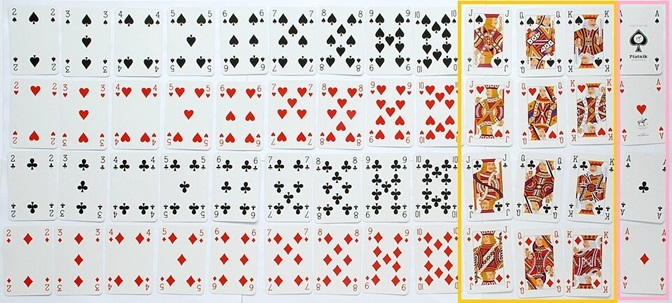
\includegraphics{images/02-cardsBC.jpg}
\caption{\label{fig:cardsBC}Events B, C (in gold and pink respectively)}
\end{figure}

Applying this idea to equation \eqref{eq:union}, we have the following for disjoint events: \textbf{for disjoint events, the probability of at least one event happening is the sum of the probabilities for each event}.

\subsection{Axioms of Probability}\label{axioms-of-probability}

The following are called the axioms of probability, which are considered foundation properties associated with probability:

\begin{enumerate}
\def\labelenumi{\arabic{enumi}.}
\tightlist
\item
  The probability of any event, \(E\), is non negative, i.e.~\(P(E) \geq 0\).
\item
  The probability that at least one outcome in the sample space occurs is 1, i.e.\(P(S) = 1\).
\item
  If \(A_1, A_2, \cdots\) are all disjoint events, then
\end{enumerate}

\[
P(\bigcup\limits_{i=1}^{\infty} A_{i}) = \sum_{i=1}^{\infty} P(A_i).
\]
In other words, for disjoint events, the probability that at least one event happens is the sum of their individual probabilities.

Note: most writers list these as three axioms. Our book combines the first two axioms into 1, and so write these as two axioms.

We can easily see how equations \eqref{eq:comp} and \eqref{eq:union} can be derived from these axioms. Note that these equations and the axioms apply in all circumstances, regardless of whether the sample space is finite or not.

\section{Conditional Probability}\label{condprob}

The concept of conditional probability appears in almost all statistical and data science models. In statistical models such as logistic regression, we are trying to use observable data (called predictors, input variables, etc) to model the probabilities associated with the different values of an outcome that is random (called response variable, output variable, etc). If the observable data are predictive of the outcome, then the probabilities associated with the outcome should indicate greater certainty, than if we do not have the observable data. Conditional probabilities allows us to incorporate observable data, or evidence, when evaluating uncertainty with random outcomes.

Consider that we are headed out for lunch, and we need to decide if we want to bring an umbrella (assuming we only bring an umbrella if we think it is going to rain). If we had been working in a windowless basement with no internet, we will have a high degree of uncertainty when evaluating if it will rain or not. However, if we were to look outside and observe the current weather conditions before heading out, we are likely to have a higher degree of certainty when evaluating if it will rain or not. Conditional probabilities allow us to incorporate what we see into our prediction of a random event.

If we were to use the language of probability to denote this example, let \(R\) denote the event that it will rain when we go for lunch. If we had been working in the windowless basement with no internet, we will be calculating \(P(R)\), the probability it will rain when we go to lunch. If we are able to incorporate the current weather conditions, this probability will be denoted as \(P(R|data)\), where data denotes the current observe weather conditions. \(P(R|data)\) can be read as the probability that it will rain when we go to lunch, given what we have observed with the weather. With this example, we can see that \(P(R)\) and \(P(R|data)\) will be different, since we update our probability given useful information. Notice the \(|\) symbol inside the probability. This symbol implies that we are working with a conditional probability, with the given or observed information listed after the \(|\).

\subsection{Definition}\label{def}

If \(X\) and \(Y\) are events, with \(P(X)>0\), the conditional probability of \(Y\) given \(X\), denoted by \(P(Y|X)\), is

\begin{equation} 
P(Y|X) = \frac{P(Y \cap X)}{P(X)}.
\label{eq:cond}
\end{equation}

In this definition, we want to update the probability of \(Y\) happening, given that we have observed \(X\). \(X\) can be viewed as the observable data or the evidence we want to incorporate.

In the Bayesian viewpoint of probability, \(P(Y)\) is called the \textbf{prior} probability of \(Y\) since it reflects our belief about \(Y\) before observing any data. \(P(Y|X)\) is called the \textbf{posterior} probability of \(Y\), as it reflects an update on our belief about \(Y\) after incorporating observed data.

Let us go back to the standard deck of cards example. Let us find \(P(B|A)\), the probability that our card is a picture card, given that we know the card is a black suit. Visually, we can use the definition of conditional probability using Figure \ref{fig:cardscond} below.

\begin{figure}
\centering
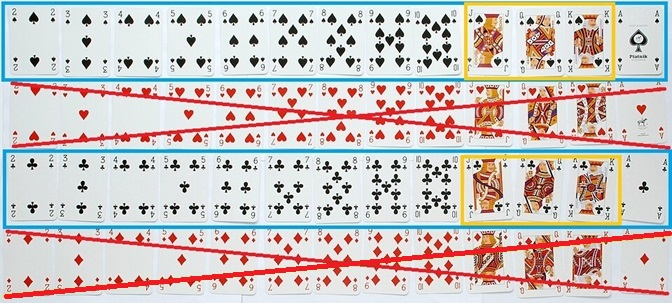
\includegraphics{images/02-cardscond.jpg}
\caption{\label{fig:cardscond}Events A, given B}
\end{figure}

We are told that our card is a black suit, so we have only 26 possible outcomes to consider, as the red cards are eliminated and are crossed out in Figure \ref{fig:cardscond}. Out of these 26 outcomes, how many are picture cards? So this probability \(P(B|A)\) is \(\frac{6}{26}\). Figure \ref{fig:cardscond} represents the frequentist viewpoint of conditional probability: \(P(B|A)\) represents the long run proportion of picture cards among cards that are black suits.

We can also apply equation \eqref{eq:cond}: \(P(B|A) = \frac{\frac{6}{52}}{\frac{1}{2}} = \frac{6}{26}\) which gives the same answer.

The video explains conditional probability with this example in a bit more detail:

\emph{Thought question}: work out the probability that the card drawn is a black suit, given that we know the card is a picture card.

We can see from this example that in general \(P(Y|X) \neq P(X|Y)\). This informs us that we need to be extremely careful when writing out our conditional probabilities and interpreting them, and knowing which one matters to our analysis. For example, the probability that I feel unwell given that I have the flu is close to 1, but the probability that I have the flu given that I feel unwell is not close to 1 (since there are many things that can make me feel unwell). This confusion regarding conditional probabilities is sometimes called the confusion of the inverse or the prosecutor's fallacy. This fallacy wrongly assumes that if the probability of a fingerprint match given that the person is innocent is small, it means that the probability that the person is innocent given a fingerprint match must also be small. Before going over this fallacy in more detail, we need to cover a few more concepts.

\subsection{Multiplication Rule}\label{multiplication-rule}

From equation \eqref{eq:cond}, we have the \textbf{multiplication rule} in probability:

\begin{equation} 
P(Y \cap X) = P(Y|X) \times P(X) = P(X|Y) \times P(Y).
\label{eq:mult}
\end{equation}

The multiplication rule is useful in finding the probability of multiple events happening, aespecially if the events happen sequentially. As an example, consider drawing two cards, without replacement, from a standard deck of cards. Without replacement means that after drawing the first card, it is not returned to the deck, so there will be 51 cards remaining after the first draw. Let \(D_1\) and \(D_2\) denote the events that the first draw is a diamond suit and the second draw is a diamond suit respectively. We want to find the probability that both cards drawn are diamond suits. This probability can be written as \(P(D_1 \cap D_2) = P(D_1) \times P(D_2|D_1)  = \frac{13}{52} \times \frac{12}{51}  = \frac{156}{2652}\).

\subsection{Independent Events}\label{independent-events}

Events are independent if knowledge about whether one event happens or not does not change the probability of the other event happening. This implies that if \(X\) and \(Y\) are independent events, then the definition of conditional probability simplifies to \(P(Y|X) = P(Y)\). Likewise \(P(X|Y) = P(X)\). Applying this to the multiplication rule, we have the following for multiplication rule for independent events

\begin{equation} 
P(Y \cap X) = P(Y) \times P(X).
\label{eq:mult2}
\end{equation}

The probability of all events happening is just the product of the probabilities for each individual event, if the events are all independent.

Going back to our example with the standard deck of cards, where \(A\) denotes the event that I draw a card with a black suit (spades or clubs), and \(B\) denotes the event I draw a picture card (Jack, Queen, or King). We had earlier found that \(P(B) = \frac{12}{52}\) and that \(P(B|A) = \frac{6}{26}\). Notice that these two probabilities are numerically equal, which informs us that the events are independent. Knowing whether the card is a black suit or not does not change the probability that the card is a picture card. This makes sense intuitively since the proportion of cars that are picture is the same for black and red suits.

\subsection{Bayes' Rule}\label{bayes-rule}

The definition of conditional probability in equation \eqref{eq:cond} and the multiplication rule in equation \eqref{eq:mult} give us \textbf{Bayes' rule}

\begin{equation} 
P(Y|X) = \frac{P(X|Y)P(Y)}{P(X)}.
\label{eq:bayes}
\end{equation}

Bayes' rule is useful if we want to find \(P(Y|X)\) but we only have information regarding \(P(X|Y)\) available. A fairly popular model is called linear discriminant analysis, and it models the conditional probability using Bayes' rule.

\subsection{Odds}\label{odds}

The \textbf{odds} of an event \(Y\) are

\begin{equation} 
odds(Y) = \frac{P(Y)}{P(Y^c)}.
\label{eq:odds}
\end{equation}

You may realize that the left hand side of equation \eqref{eq:odds} is equal to the left hand side of a logistic regression equation that we saw in Section \ref{eg2}.

Using equation \eqref{eq:odds}, we can switch from odds to probability easily

\begin{equation} 
P(Y) = \frac{odds(Y)}{1 + odds(Y)}.
\label{eq:odds2}
\end{equation}

\subsection{Odds Form of Bayes' Rule}\label{odds-form-of-bayes-rule}

Using Bayes' rule in equation \eqref{eq:bayes} and the definition of odds in equation \eqref{eq:odds}, we have the \textbf{odds form for Bayes' rule}

\begin{equation} 
\frac{P(Y|X)}{P(Y^c|X)} = \frac{P(X|Y)}{P(X|Y^c)} \frac{P(Y)}{P(Y^c)}. 
\label{eq:oddsbayes}
\end{equation}

\subsection{Law of Total Probability}\label{law-of-total-probability}

Let \(Y_1, Y_2, \cdots, Y_n\) be a partition of the sample space (\(Y_1, Y_2, \cdots, Y_n\) are disjoint and their union is the sample space, with \(P(Y_i) > 0\)) for all \(i\). Then

\begin{equation} 
\begin{split}
P(X) &= \sum_{i=1}^n P(X|Y_i) \times P(Y_i)\\
    &= P(X|Y_1) \times P(Y_1) + P(X|Y_2) \times P(Y_2) + \cdots + P(X|Y_n) \times P(Y_n).
\end{split}
\label{eq:total}
\end{equation}

The law of total probability informs us of a way to find the probability of \(X\). We can divide the sample space in disjoint sets \(Y_i\), find the conditional probability of \(X\) within each set, and then take a weighted sum of these conditional probabilities, weighted by \(P(Y_i)\). This is useful if the conditional probability for each set is easy to obtain.

The law of total probability in equation \eqref{eq:total} can be applied to the denominator of Bayes' rule in equation \eqref{eq:bayes} to have the following variation of Bayes' rule:

\begin{equation} 
P(Y|X) = \frac{P(X|Y)P(Y)}{\sum_{i=1}^n P(X|Y_i) \times P(Y_i)}.
\label{eq:bayes2}
\end{equation}

\subsection{Worked Example}\label{worked-example}

We consider this worked example on how to apply Bayes' rule and the law of total probability. Suppose my email can be divided into three categories: \(E_1\) denotes spam email, \(E_2\) denotes important email, and \(E_3\) denotes not important email. An email must belong to only one of these categories. Let \(F\) denote the event that the email contains the word ``free''. From past data, I have the following information:

\begin{itemize}
\tightlist
\item
  \(P(E_1) = 0.2, P(E_2) = 0.5, P(E_3) = 0.3\).
\item
  The word ``free'' appears in 99\% of spam email, so \(P(F|E_1) = 0.99\).
\item
  The word ``free'' appears in 10\% of important email, so \(P(F|E_2) = 0.1\).
\item
  The word ``free'' appears in 5\% of not important email, so \(P(F|E_3) = 0.05\).
\end{itemize}

I receive an email that has the word free. What is the probability that it is spam? So we want to find \(P(E_1|F)\).

\subsubsection{Approach 1: Using Bayes' Rule}\label{approach-1-using-bayes-rule}

Using equation \eqref{eq:bayes2}, we have

\[
\begin{split}
P(E_1|F) &= \frac{P(E_1 \cap F)}{P(F)}\\
 &= \frac{P(F|E_1) \times P(E_1)}{P(F|E_1) \times P(E_1) + P(F|E_2) \times P(E_2) + P(F|E_3) \times P(E_3)} \\
&= \frac{0.99 \times 0.2}{0.99 \times 0.2 + 0.1 \times 0.5 + 0.05 \times 0.3}\\
&= 0.7528517
\end{split}
\]

The video below goes over this approach in a little bit more detail:

\subsubsection{Approach 2: Using Tree Diagrams}\label{approach-2-using-tree-diagrams}

A tree diagram is useful in finding conditional probabilities and probabilities involving intersections. It is a visual way of displaying the information you have at hand, when you have conditional probabilities over disjoint sets and probabilities for each disjoint set. In our toy example, the disjoint sets are the type of email I receive, \(E_1, E_2, E_3\), and the conditional probabilities we have are over these disjoint sets, i.e.~\(P(F|E_1), P(F|E_2)\) and \(P(F|E_3)\). We can put this information visual by first splitting our sample space into the disjoint sets \(E_1, E_2, E_3\), and then splitting each disjoint set on whether the email has the word ``free'' (\(F\)) or not (\(F^c\)). This information is displayed in a tree diagram as in Figure \ref{fig:tree}.

\begin{figure}
\centering
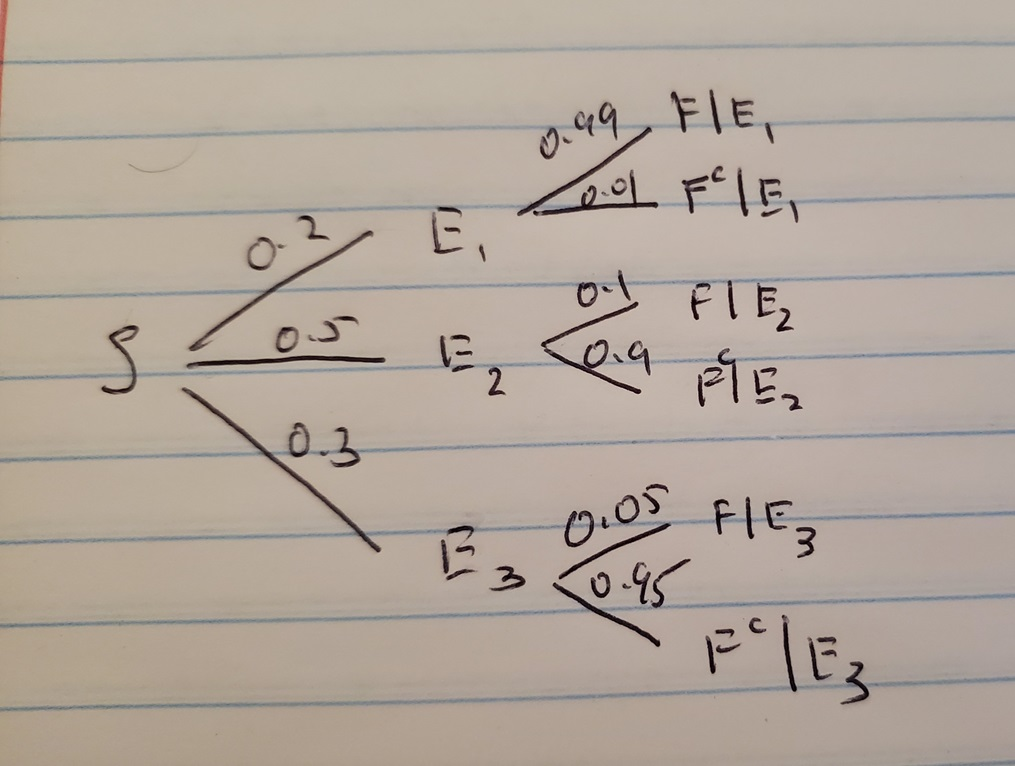
\includegraphics{images/02-tree.jpg}
\caption{\label{fig:tree}Tree Diagram for Email Example}
\end{figure}

Each split is represented by a branch, and we write the corresponding probability on each branch. We want to find the probability that a received email is spam given that it contains the word ``free'', \(P(E_1|F)\), and using the definition of conditional probability in equation \eqref{eq:cond}

\[
P(E_1|F) = \frac{P(E_1 \cap F)}{P(F)}.
\]

Looking at the tree diagram in Figure \ref{fig:tree}, we can label the branches that lead to the numerator \(P(E_1 \cap F)\), the probability that the email is spam and contains the word free. This is shown on the tree diagram below in Figure \ref{fig:tree1} below by highlighting the corresponding branches in blue.

\begin{figure}
\centering
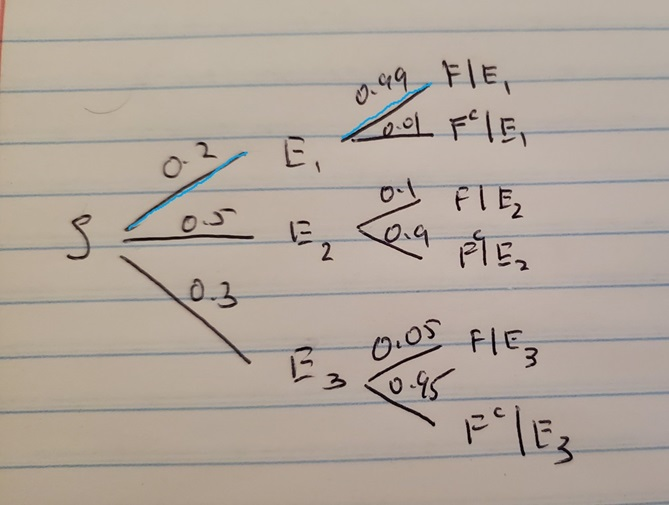
\includegraphics{images/02-treepath1.jpg}
\caption{\label{fig:tree1}Tree Diagram for Email Example, Branch for Numerator in Blue}
\end{figure}

So \(P(E_1 \cap F) = 0.2 \times 0.99 = 0.198\). We then need to find the denominator \(P(F)\). Looking at Figure \ref{fig:tree}, we can see three branches that lead to an email containing the word free: \(P(E_1 \cap F)\) or \(P(E_2 \cap F)\) or \(P(E_3 \cap F)\). This is shown on the tree diagram below in Figure \ref{fig:tree2} below by highlighting the corresponding branches in gold.

\begin{figure}
\centering
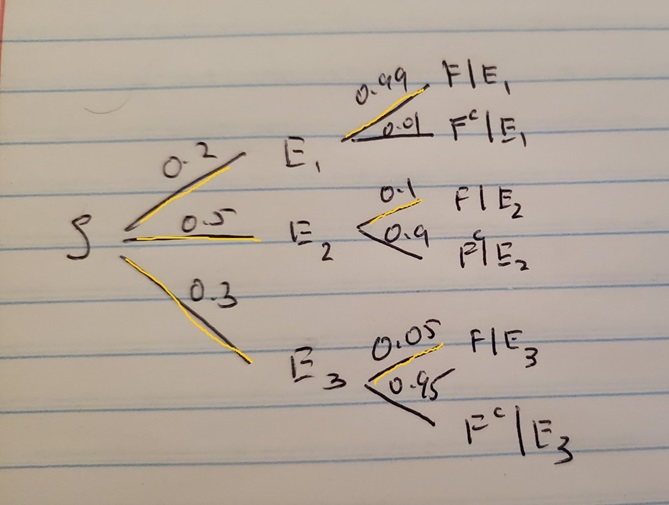
\includegraphics{images/02-treepath2.jpg}
\caption{\label{fig:tree2}Tree Diagram for Email Example, Branches for Denominator in Gold}
\end{figure}

We know the probability for each branch, and we add them up to obtain the denominator \(P(F) = 0.2 \times 0.99 + 0.5 \times 0.1 + 0.3 \times 0.05 = 0.263.\) Putting the pieces together, we have

\[
P(E_1|F) = \frac{P(E_1 \cap F)}{P(F)} = \frac{0.198}{0.263} = 0.7528517.
\]

Note: If you compare the intermediate calculations in approach 2, you end up using the calculations in approach 1, without referring to any of the associated equations.

The video below goes over tree diagrams in a little bit more detail:

\section{Confusion of the Inverse}\label{confusion-of-the-inverse}

We are now ready to talk about the prosecutor's fallacy, or the \textbf{confusion of the inverse}, that we had earlier mention in section \ref{def}. In essence, the confusion happens when we falsely equate \(P(X|Y)\) to be equal to \(P(Y|X)\). In fact, a large value for \(P(X|Y)\) does not necessarily imply that \(P(Y|X)\) is also large. The term prosecutor's fallacy when this confusion is applied in a criminal trial, e.g.~the probability that an abusive relationship ends in murder could be small, but the probability that there was abuse in a relationship that ended in murder could be a lot higher.

We will go over some examples that are based on real life.

\subsection{Disease Diagnostics}\label{disease-diagnostics}

Suppose we are testing a patient if he has a rare disease, which is estimated to be prevalent in 0.5\% of all people. Suppose we have a medical test for this disease that is accurate. There can be a number of definitions of accuracy. In disease diagnostics, a couple of measures are sensitivity, which is the proportion of people with the disease who test positive, and specificity, the proportion of people without the disease who test negative. A positive test indicates the person has the disease. Suppose the sensitivity and specificity are both high: 0.95 and 0.9 respectively. Suppose the patient tests positive, what is the probability that the patient actually has the disease? Assume the test always indicates positive or negative.

For this example, let \(D\) denote the event the patient has the disease, and let + denote the event the patient tests positive on the test, and - denote the event the patient tests negative on the test. Given the information, we have

\begin{itemize}
\tightlist
\item
  \(P(D) = 0.005\).
\item
  \(P(+|D) = 0.95\).
\item
  \(P(-|D^c) = 0.9\).
\end{itemize}

We wish to find \(P(D|+)\). Using Bayes rule and the Law of Total probability, this is

\[
\begin{split}
P(D|+) &= \frac{P(D \cap +)}{P(+)}\\
 &= \frac{P(+|D) \times P(D)}{P(+|D) \times P(D) + P(+|D^c) \times P(D^c)} \\
&= \frac{0.95 \times 0.005}{0.95 \times 0.005 + 0.1 \times 0.995 }\\
&= 0.04556355
\end{split}
\]

which is a small probability, so the patient is highly unlikely to actually have the rare disease. So while the test has high sensitivity with \(P(+|D) = 0.95\), this does not imply that a patient who tests positive actually has the disease, since \(P(D|+)\) is low. The implication is that for a rare disease, a positive test does not imply you have a high probability of having the disease, even if the test is accurate.

Why does this result make sense? Essentially, a large proportion of a small population could still be numerically much smaller than a small proportion of a large population. The disease is rare, so we have a small population of people with the disease, and almost all of them are detected by the test. We also have an extremely large population of people without the disease, and even a small proportion of them who erroneously test positive could still be a fairly large number. So among all the positive tests, most of the people do not have the disease. We consider the following table based on a population of 20 thousand people, in Table \ref{tab:disease} below:

\begin{longtable}[]{@{}cccc@{}}
\caption{\label{tab:disease} Hypothetical Table Based on 20,000 People}\tabularnewline
\toprule\noalign{}
& Positive & Negative & Total \\
\midrule\noalign{}
\endfirsthead
\toprule\noalign{}
& Positive & Negative & Total \\
\midrule\noalign{}
\endhead
\bottomrule\noalign{}
\endlastfoot
Disease & 95 & 5 & 100 \\
No Disease & 1990 & 17910 & 19900 \\
Total & 2085 & 17915 & 20000 \\
\end{longtable}

Look at the first column of Table \ref{tab:disease}, which shows number of people who test positive. A see that a large proportion of diseased people are detected, but since there are relatively few people with the disease, this number is small, 95. A small proportion of people who do not have the disease test positive for the disease, and a small proportion of this large population results in a relatively larger number, 1990. So most of the people who test positive, \(95 + 1990 = 2085\) actually do not have the disease. Therefore \(P(D|+) = \frac{95}{2085} = 0.04556355\).

We can also explain this result through the Bayes' viewpoint of probability. Without knowing any information about the results of the test, the prior probability \(P(D) = 0.005\). However, upon seeing that the person positive, we updated the posterior probability \(P(D|+) = 0.04556355\), which is an increase from 0.005 when we knew knowing. The updated posterior probability is about 9 times the prior. So we believe the person is more likely to have the disease upon viewing the positive test, than if we knew nothing about the test result. The posterior probability is still small since its value depends on two pieces of information: the prior \(P(D)\) and the sensitivity \(P(+|D)\). The product of these values belong to the numerator when calculating \(P(D|+)\). The denominator is \(P(+|D) \times P(D) + P(+|D^c) \times P(D^c)\). If the prior \(P(D)\) is extremely low, then \(P(D^c)\) is extremely close to 1, since the person either has the disease or does not have the disease. With \(P(D)\) belong extremely low, the numerator is close to 0, and the value of the denominator is close to \(P(+|D^c) \times P(D^c)\), therefore \(P(D|+)\) is small.

Notice how we have talking about rare diseases? This confusion of the inverse, thinking that a high sensitivity implies that a person likely to have the disease if they test positive, only applies to rare diseases. If the disease is more prevalent, a high sensitivity is more likely to imply the person has the disease if they test positive.

So why should we take such tests for rare diseases? What should we do? We should go through the test again. It turns out that if you test positive twice for a rare disease, the probability that you have the disease increases by a lot than if you only tested once and tested positive.

To perform this calculation, we will use the odds form for Bayes' rule, per equation \eqref{eq:oddsbayes}

\[
\begin{split}
\frac{P(D|T_1 \cap T_2)}{P(D^c|T_1 \cap T_2)} &= \frac{P(T_1 \cap T_2 | D)}{P(T_1 \cap T_2 | D^c)} \frac{P(D)}{P(D^c)}\\
 &= \frac{0.95^2}{0.1^2} \frac{0.005}{0.995} \\
&= 0.4535176
\end{split}
\]

where \(T_1\) and \(T_2\) denote the events the person test positive in the first test and second test respectively. We also assume that the results from each test are independent with previous tests.

The odds of having the disease given that the person positive twice is 0.4535176. Therefore, using equation \eqref{eq:odds2}, the corresponding probability of having the disease given that the person tested positive twice is \(P(D|T_1 \cap T_2) = \frac{0.4535176}{1+0.4535176} = 0.3120138\). See how this posterior probability has increased with two positive tests, from 1 positive test.

\emph{Thought question}: perform the calculations to show that the posterior probability that the person has the disease if the person tests positive on 3 tests is 0.8116199.

\emph{Thought question}: do you notice a certain pattern emerging when performing these calculations as the person undergoes more tests? Could you write either a mathematical equation, or even a function in R, that allows us to quickly compute the probability the person has the disease given that the person tested positive \(k\) times, where \(k\) can denote any non negative integer?

\subsection{Prosecutor's Fallacy}\label{prosecutors-fallacy}

The confusion of the inverse is also called the prosecutor's fallacy (sometimes also called the defense attorney's fallacy depending on which side is making the mistake) when it occurs in a legal setting. Generally, the confusion comes from equating P(evidence\textbar innocent) with P(innocent\textbar evidence).

The book provides a discussion about this in Section 2.8, examples 2.8.1 and 2.8.2.

\chapter{Discrete Random Variables}\label{discrete-random-variables}

This module is based on Introduction to Probability (Blitzstein, Hwang), Chapters 3 and 4. You can access the book for free at \url{https://stat110.hsites.harvard.edu/} (and then click on Book). Please note that I cover additional topics, and skip certain topics from the book. You may skip Sections 3.4, 3.9, Example 4.2.3, Section 4.3, Example 4.4.6, 4.4.7, Theorem 4.4.8, Example 4.4.9, 4.6.4, 4.7.4, 4.7.7, and Section 4.9 from the book.

\section{Random Variables}\label{random-variables}

The idea behind random variables is to simplify notation regarding probability, enable us to summarize results of experiments, and make it easier to quantify uncertainty.

\subsection{Example}\label{example}

Consider flipping a coin three times and recording if it lands heads or tails each time. The sample space for this experiment will be \(S = \{HHH, HHT, HTH, THH, HTT, THT, TTH, TTT\}\). Given that each outcome is equally likely, the probability associated with each outcome is \(\frac{1}{8}\).

Suppose I want to find the probability that I get exactly 2 heads out of the 3 flips. I could express this as:

\begin{itemize}
\tightlist
\item
  \(P(\text{two heads out of three flips})\), or
\item
  \(P(HHT \cup HTH \cup THH)\), or
\item
  \(P(A)\) where \(A\) denotes the event of getting two heads out of three flips.
\end{itemize}

Another way is to define a random variable \(X\) that expresses this event a bit more efficiently. Let \(X\) denote the number of heads out of three flips, so another way could be to write \(P(X=2\)). This is the idea behind random variables: to assign events to a number.

\subsection{Definition}\label{definition}

A \textbf{random variable (RV)} is a function from the sample space to real numbers.

By convention, we denote random variables by capital letters. Using our 3 coin flip example, \(X\) could be 0, 1, 2, or 3. We assign a number to each possible outcome of the sample space.

Random variables provide numerical summaries of the experiment. This can be useful especially if the sample space is complicated. Random variables can also be used for non numeric outcomes.

\subsection{Discrete Vs Continuous}\label{discrete-vs-continuous}

One of the key distinctions we have to make for random variables is to determine if it is discrete or continuous. The way we express probabilities for random variables depends on whether the random variable is discrete or continuous.

A \textbf{discrete random variable} can only take on a countable (finite or infinite) number of values.

The number of heads in 3 coin flips, \(X\) is \textbf{countable and finite}, since we can actually list all of the values it can take as \(\{0,1,2,3 \}\) and there are 4 such values. \(X\) must take on one of these 4 numerical values; it cannot be a number outside this list. So it is discrete.

A random variable is \textbf{countable and infinite} if we can list the values it can take, but the list has no end. For example, the number of people using a crosswalk over a 10 year period could take on the values \(\{0, 1, 2, 3, \cdots \}\). The number could take on any of an infinite number of values, but values in between these whole numbers cannot occur. So the number of people using a crosswalk over a 10 year period is a discrete random variable.

A \textbf{continuous random variable} can take on an uncountable number of values in an interval of real numbers.

For example, height of an American adult is a continuous random variable, as height can take on any value in interval between any interval, say 40 and 100 inches. All values between 40 and 100 are possible.

For this module, we will focus on discrete random variables.

The \textbf{support} of a discrete random variable \(X\) is the set of values \(X\) can take such that \(P(X = x) > 0\), i.e.~the set of values that have non zero probability of happening. Using our 3 coin flips example, where \(X\) is the number of heads out of the 3 coin slips, the support is \(\{0,1,2,3 \}\). he support of discrete random variables is usually integers.

\emph{Thought question}: Can you come of examples of discrete and continuous random variables on your own? Feel free to search the internet for examples as well.

\section{Probability Mass Functions (PMFs)}\label{probability-mass-functions-pmfs}

We use probability to describe the behavior of random variables. This is called the \textbf{distribution} of a random variable. The distribution of a random variable specifies the probabilities of all events associated with the random variable.

For discrete random variables, the distribution is specified by the \textbf{probability mass function (PMF)}. The PMF of a discrete random variable \(X\) is the function \(P_X(x) = P(X=x)\). It is positive when \(x\) is in the support of \(X\), and 0 otherwise.

Note: In the notation for random variables, capital letters such as \(X\) denote random variables, and lower case letters such as \(x\) denote actual numerical values. So if we want to find the probability that we have 2 heads in 3 coin flips, we write \(P(X=2)\), where \(x\) is 2 in this example.

Going back to our example where we record the number of heads out of 3 coin flips, we can write out the PMF for the random variable \(X\):

\begin{itemize}
\tightlist
\item
  \(P_X(0) = P(X=0) = P(TTT) = \frac{1}{8}\),
\item
  \(P_X(1) = P(X=1) = P(HTT \cup THT \cup TTH) = \frac{3}{8}\),
\item
  \(P_X(2) = P(X=2) = P(HHT \cup THH \cup HTH) = \frac{3}{8}\),
\item
  \(P_X(3) = P(X=3) = P(HHH) = \frac{1}{8}\).
\end{itemize}

Fairly often, the PMF of a discrete random variable is presented in a simple table like in Table \ref{tab:3-pmf-tab} below:

\begin{table}

\caption{\label{tab:3-pmf-tab}PMF for X}
\centering
\begin{tabular}[t]{r|r}
\hline
x & PMF\\
\hline
0 & 0.125\\
\hline
1 & 0.375\\
\hline
2 & 0.375\\
\hline
3 & 0.125\\
\hline
\end{tabular}
\end{table}

Or the PMF can be represented using a simple plot like the one below in Figure \ref{fig:3-pmf}:

\begin{Shaded}
\begin{Highlighting}[]
\DocumentationTok{\#\#support}
\NormalTok{x}\OtherTok{\textless{}{-}}\DecValTok{0}\SpecialCharTok{:}\DecValTok{3}
\DocumentationTok{\#\# PMF for each value in the support. }
\NormalTok{PMFs}\OtherTok{\textless{}{-}}\FunctionTok{c}\NormalTok{(}\DecValTok{1}\SpecialCharTok{/}\DecValTok{8}\NormalTok{, }\DecValTok{3}\SpecialCharTok{/}\DecValTok{8}\NormalTok{, }\DecValTok{3}\SpecialCharTok{/}\DecValTok{8}\NormalTok{, }\DecValTok{1}\SpecialCharTok{/}\DecValTok{8}\NormalTok{)}
\DocumentationTok{\#\# create plot of PMF vs each value in support}
\FunctionTok{plot}\NormalTok{(x, PMFs, }\AttributeTok{type=}\StringTok{"h"}\NormalTok{, }\AttributeTok{main =} \StringTok{"PMF for X"}\NormalTok{, }\AttributeTok{xlab=}\StringTok{"\# of heads"}\NormalTok{, }\AttributeTok{ylab=}\StringTok{"Probability"}\NormalTok{, }\AttributeTok{ylim=}\FunctionTok{c}\NormalTok{(}\DecValTok{0}\NormalTok{,}\DecValTok{1}\NormalTok{))}
\end{Highlighting}
\end{Shaded}

\begin{figure}
\centering
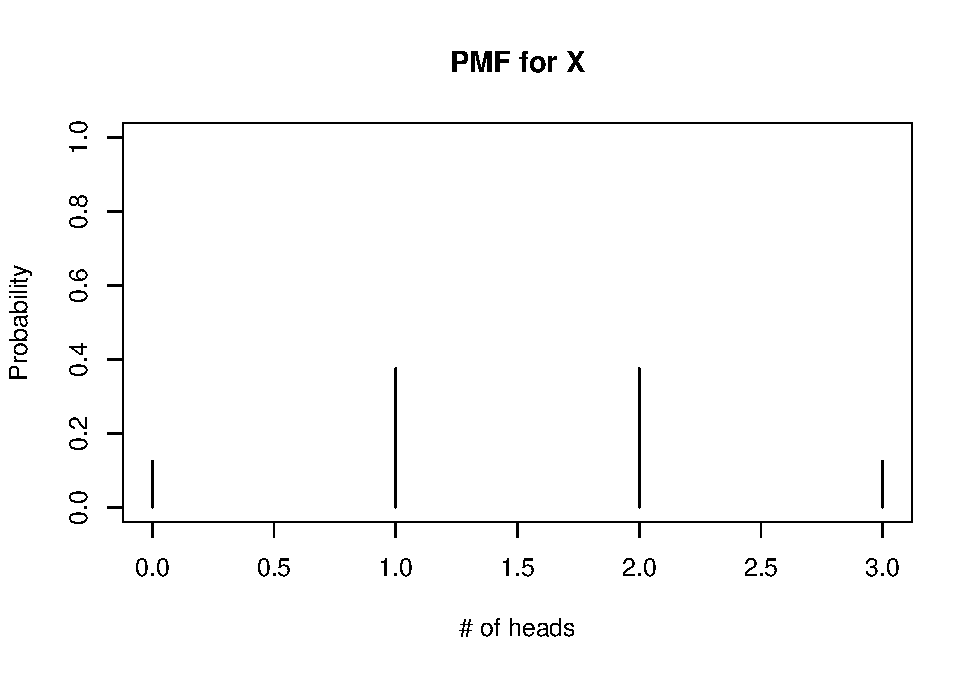
\includegraphics{bookdown-demo_files/figure-latex/3-pmf-1.pdf}
\caption{\label{fig:3-pmf}PMF for X}
\end{figure}

The PMF provides a list of all possible values for the random variable and the corresponding probabilities. In other words, the PMF describes the distribution of the relative frequencies for each outcome. For our experiment, observing 1 or 2 heads is equally likely, and they occur three times as often as observing 0 or 3 heads. Observing 0 or 3 heads is also equally likely.

\subsection{Valid PMFs}\label{valid-pmfs}

Consider a discrete random variable \(X\) with support \(x_1, x_2, \cdots\). The PMF \(P_X(x)\) of \(X\) must satisfy:

\begin{itemize}
\tightlist
\item
  \(P_X(x) > 0\) if \(x = x_j\), and \(P_X(x) = 0\) otherwise.
\item
  \(\sum_{j=1}^{\infty} P_X(x_j) = 1\).
\end{itemize}

In other words, the probabilities associated with the support are greater than 0, and the sum of the probabilities across the whole support must add up to 1.

\emph{Thought question}: based on Table \ref{tab:3-pmf-tab}, can you see why our PMF for \(X\) is valid?

\subsection{PMFs and Histograms}\label{pmfhist}

Recall the frequentist viewpoint of probability, that it represents the relative frequency associated with an event that is repeated for an infinite number of times.

Consider our experiment where we flip a coin 3 times and count the number of heads. The support of our random variable \(X\), the number of heads, is \(\{0,1,2,3 \}\). Imagine performing our experiment a large number of times. Each time we perform the experiment, we record the number of heads. If we performed the experiment one million times, we would have recorded one million values for the number of heads, and each value must be in the support of \(X\). If we then create a histogram for the one million values for the number of heads, the shape of the histogram should be very close to the shape of the plot of the PMF in Figure \ref{fig:3-pmf}. Figure \ref{fig:3-sim} below shows the resulting histogram after performing the experiment 1 million times.

\begin{figure}
\centering
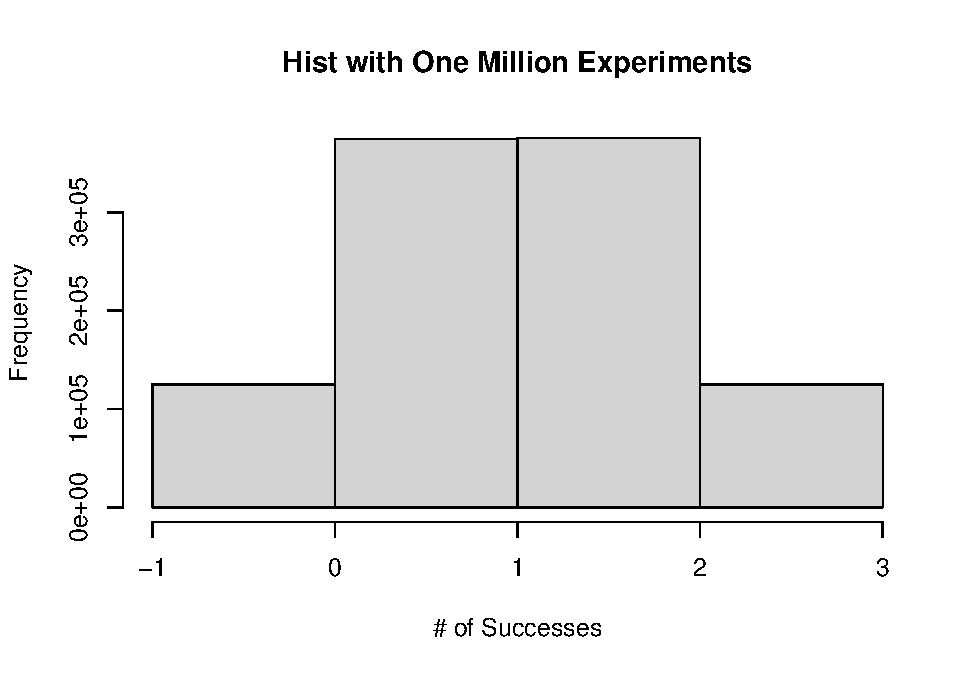
\includegraphics{bookdown-demo_files/figure-latex/3-sim-1.pdf}
\caption{\label{fig:3-sim}Histogram from Experiment Performed 1 Million Times}
\end{figure}

In general, the PMF of a random variable should match the histogram in the long run.

Note: What we have just done here was to use simulations to repeat an experiment a large number of times.

\section{Cumulative Distribution Functions (CDFs)}\label{cumulative-distribution-functions-cdfs}

Another function that is used to describe the distribution of discrete random variables is the \textbf{cumulative distribution function (CDF)}. The CDF of a random variable \(X\) is \(F_X(x) = P(X \leq x)\). Notice that unlike the PMF, the definition of CDF applies for both discrete and continuous random variables.

Going back to our example where we record the number of heads out of 3 coin flips, we can write out the CDF for the random variable \(X\):

\begin{itemize}
\tightlist
\item
  \(F_X(0) = P(X \leq 0) = P(X=0) = \frac{1}{8}\),
\item
  \(F_X(1) = P(X \leq 1) = P(X=0) + P(X=1) = \frac{1}{8} +  \frac{3}{8} = \frac{1}{2}\),
\item
  \(F_X(2) = P(X \leq 2) = P(X=0) + P(X=1) + P(X=2) = \frac{1}{2} + \frac{3}{8} = \frac{7}{8}\),
\item
  \(F_X(3) = P(X \leq 3) = P(X=0) + P(X=1) + P(X=2) + P(X=3) = \frac{7}{8} + \frac{1}{8} = 1\).
\end{itemize}

Notice how these calculations were based on the PMF. To find \(P(X \leq x)\), we summed the PDF over all values of the support that is less than or equal to \(x\). Therefore, another way to write the CDF for a discrete random variable is

\begin{equation} 
F_X(x) = P(X \leq x) = \sum_{x_j \leq x} P(X=x_j).
\label{eq:3-CDF}
\end{equation}

Fairly often, the CDF of a discrete random variable is presented in a simple table like Table \ref{tab:3-cdf-tab} below:

\begin{table}

\caption{\label{tab:3-cdf-tab}CDF for X}
\centering
\begin{tabular}[t]{r|r}
\hline
x & CDF\\
\hline
0 & 0.125\\
\hline
1 & 0.500\\
\hline
2 & 0.875\\
\hline
3 & 1.000\\
\hline
\end{tabular}
\end{table}

Or in a simple plot like in Figure \ref{fig:3-cdf} below:

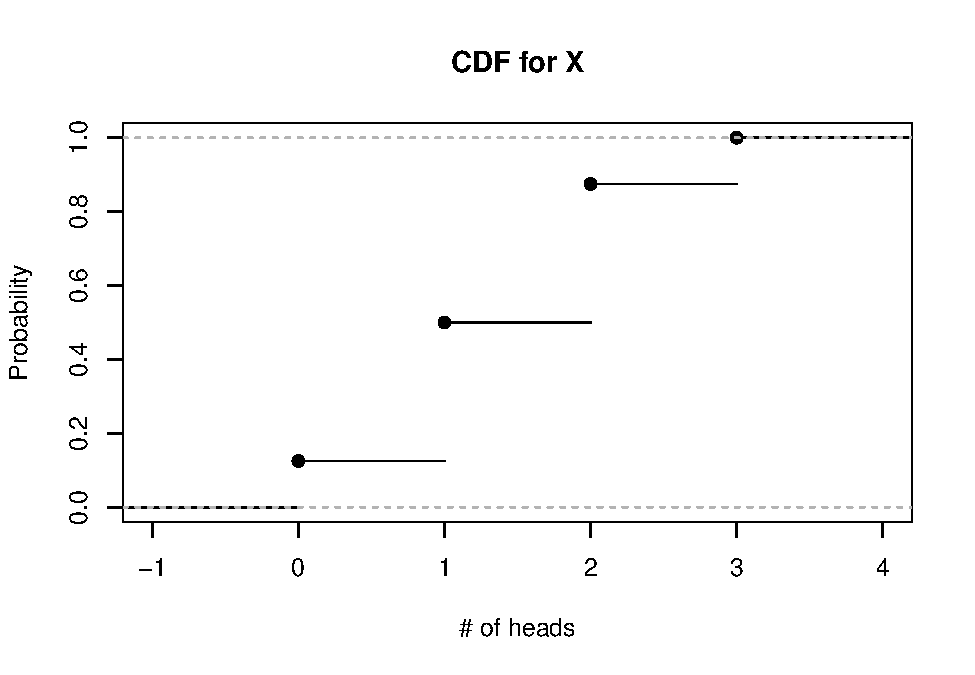
\includegraphics{bookdown-demo_files/figure-latex/3-cdf-1.pdf}
The CDF for discrete random variables always look like a step function, as it increases in discrete jumps at each value of the support. The height of each jump corresponds to the PMF at that value of the support.

\emph{Thought question}: do you see similarities between the CDF and the empirical cumulative density function (ECDF) from section \ref{ecdf}?

\subsection{Valid CDFs}\label{valid-cdfs}

The CDF \(F_X(x)\) of \(X\) must:

\begin{itemize}
\tightlist
\item
  be non decreasing. This means that as \(x\) gets larger, the CDF either stays the same or increases. Visually, a graph of the CDF never decreases as \(x\) increases.
\item
  approach 1 as \(x\) approaches infinity and approach 0 as \(x\) approaches negative infinity. Visually, a graph of the CDF should be equal to or close to 1 for large values of x, and it should be equal to or close to 0 for small values of x.
\end{itemize}

\emph{Thought question}: Look at the CDF for our example in Figure \ref{fig:3-cdf}, and see how it satisfies the criteria listed above for a valid CDF.

\section{Expectations}\label{expectations}

In the previous section, we see how PMFs and CDFs can be used to describe the distribution of a random variable. As the PMF can be viewed as a long-run version of the histogram, it gives us an idea about the shape of the distribution. Similar to Section \ref{descriptive}, we will also be interested in measures of centrality and spread for random variables.

A measure of centrality for random variables is the \textbf{expectation}, or \textbf{expected value}. The expectation of a random variable can be interpreted as the long-run mean of the random variable, i.e.~if we were able to repeat the experiment an infinite number of times, the expectation of the random variable will be the average result among all the experiments.

For a discrete random variable \(X\) with support \(x_1, x_2, \cdots,\), the expected value, denoted by \(E(X)\), is

\begin{equation} 
E(X) = \sum_{j=1}^{\infty} x_j P(X=x_j).
\label{eq:3-EX}
\end{equation}

We can use Table \ref{tab:3-pmf-tab} as an example. To find the expected number of heads out of 3 coin flips, using equation \eqref{eq:3-EX},

\[
\begin{split}
E(X) &= 0 \times \frac{1}{8} + 1 \times \frac{3}{8} + 2 \times \frac{3}{8} + 3 \times \frac{1}{8}\\
       &= 1.5
\end{split}
\]

What we did was to take the product of each value in the support of the random variable with its corresponding probability, and add all these products.

We can see another interpretation of the expected value of a random variable from this calculation: it is the weighted average of the values for the random variable, weighted by their probabilities.

Intuitively, this expected value of 1.5 should make sense. If we flip a coin 3 times, and the coin is fair, we expect half of these flips to land heads, or 1.5 flips to land heads.

View the video below for a more detailed explanation on how to calculate expected values:

\subsection{Linearity of Expectations}\label{linearity-of-expectations}

We have seen how to calculate the expected value of a random variable \(X\) using equation \eqref{eq:3-EX}. What we need is the PMF of \(X\). Sometimes our random variable can be viewed as a sum (or difference) of other random variables, or it could involve a multiplication and / or adding a constant to the random variable. Consider some of these scenarios:

\begin{itemize}
\item
  Suppose my friend and I are fisherman. Let \(Y\) be the random variable describing the number of fish I catch on a workday, and let \(W\) be the random variable describing the number of fish my friend catches on a workday. We can let \(T = Y+W\) be the random variable describing the total number of fish we catch on a workday.
\item
  Suppose that I sell each fish for \$10 and my friend sells each fish for \$15. We can let \(R = 10Y + 15W\) be the random variable that describes the revenue we generate on a workday.
\item
  Suppose that my friend and I rent out a space at the market to sell our fish, and it costs \$5 a day to rent out the space. We can let \(G = 10Y + 15W - 5\) be the random variable that describes our gross income for the day.
\end{itemize}

All of these examples involve new random variables, \(T, R, G\) that can be based on previously defined random variables, \(Y, W\). It turns out that to find the expectations of the new random variables, all we need is the expectations of the previously defined random variables. We do not need to find the PMFs for \(T, R\) and \(S\) and then apply equation \eqref{eq:3-EX}.

These can be done through the \textbf{linearity of expectations}: Let \(X\) and \(Y\) denote random variables, and \(a,b,c\) denote some constants, then

\begin{equation} 
E(aX + bY + c) = aE(X) + bE(Y) + c.
\label{eq:3-linEX}
\end{equation}

Applying equation \eqref{eq:3-linEX} to the fishing examples:

\begin{itemize}
\tightlist
\item
  \(E(T) = R(Y + W) = E(Y) + E(W)\),
\item
  \(E(R) = E(10Y + 15W) = 10E(Y) + 15E(W)\),
\item
  \(E(G) = E(10Y + 15W - 5) = 10E(Y) + 15E(W) - 5\).
\end{itemize}

All we need to find the expected values for the total number of fish, revenue generated, and gross income were the expected values for the number of fish each of us caught. We do not need the PMFs for \(T,R,G\).

\subsubsection{Visual Explanation}\label{visual-explanation}

For a visual explanation of why equation \eqref{eq:3-linEX} makes sense, we go back to our previous example where \(X\) denotes the number of heads in 3 coin flips. Figure \ref{fig:3-pmf} displays the PMF for this random variable. Let us create the PMF for a new random variable \(Y=2X\) and display it in Figure \ref{fig:3-pmf-lin} below:

\begin{Shaded}
\begin{Highlighting}[]
\DocumentationTok{\#\#support of X}
\NormalTok{x}\OtherTok{\textless{}{-}}\DecValTok{0}\SpecialCharTok{:}\DecValTok{3}
\DocumentationTok{\#\# PMF for each value in the support. }
\NormalTok{PMFs}\OtherTok{\textless{}{-}}\FunctionTok{c}\NormalTok{(}\DecValTok{1}\SpecialCharTok{/}\DecValTok{8}\NormalTok{, }\DecValTok{3}\SpecialCharTok{/}\DecValTok{8}\NormalTok{, }\DecValTok{3}\SpecialCharTok{/}\DecValTok{8}\NormalTok{, }\DecValTok{1}\SpecialCharTok{/}\DecValTok{8}\NormalTok{)}
\NormalTok{EX}\OtherTok{\textless{}{-}}\FloatTok{1.5}

\DocumentationTok{\#\#support of Y}
\NormalTok{y}\OtherTok{\textless{}{-}}\DecValTok{2}\SpecialCharTok{*}\NormalTok{x}
\DocumentationTok{\#\# PMF for each value in the support. }
\NormalTok{PMFs}\OtherTok{\textless{}{-}}\FunctionTok{c}\NormalTok{(}\DecValTok{1}\SpecialCharTok{/}\DecValTok{8}\NormalTok{, }\DecValTok{3}\SpecialCharTok{/}\DecValTok{8}\NormalTok{, }\DecValTok{3}\SpecialCharTok{/}\DecValTok{8}\NormalTok{, }\DecValTok{1}\SpecialCharTok{/}\DecValTok{8}\NormalTok{)}
\NormalTok{EY}\OtherTok{\textless{}{-}}\DecValTok{2}\SpecialCharTok{*}\NormalTok{EX}

\FunctionTok{par}\NormalTok{(}\AttributeTok{mfrow=}\FunctionTok{c}\NormalTok{(}\DecValTok{2}\NormalTok{,}\DecValTok{1}\NormalTok{))}

\DocumentationTok{\#\# create plot of PMF vs each value in support}
\FunctionTok{plot}\NormalTok{(x, PMFs, }\AttributeTok{type=}\StringTok{"h"}\NormalTok{, }\AttributeTok{main =} \StringTok{"PMF for X"}\NormalTok{, }\AttributeTok{xlab=}\StringTok{"X"}\NormalTok{, }\AttributeTok{ylab=}\StringTok{"Probability"}\NormalTok{, }\AttributeTok{ylim=}\FunctionTok{c}\NormalTok{(}\DecValTok{0}\NormalTok{,}\DecValTok{1}\NormalTok{))}
\DocumentationTok{\#\#overlay a line representing EX in red}
\FunctionTok{abline}\NormalTok{(}\AttributeTok{v=}\NormalTok{EX, }\AttributeTok{col=}\StringTok{"red"}\NormalTok{)}

\DocumentationTok{\#\# create plot of PMF vs each value in support}
\FunctionTok{plot}\NormalTok{(y, PMFs, }\AttributeTok{type=}\StringTok{"h"}\NormalTok{, }\AttributeTok{main =} \StringTok{"PMF for Y"}\NormalTok{, }\AttributeTok{xlab=}\StringTok{"Y"}\NormalTok{, }\AttributeTok{ylab=}\StringTok{"Probability"}\NormalTok{, }\AttributeTok{ylim=}\FunctionTok{c}\NormalTok{(}\DecValTok{0}\NormalTok{,}\DecValTok{1}\NormalTok{))}
\DocumentationTok{\#\#overlay a line representing EY in red}
\FunctionTok{abline}\NormalTok{(}\AttributeTok{v=}\NormalTok{EY, }\AttributeTok{col=}\StringTok{"red"}\NormalTok{)}
\end{Highlighting}
\end{Shaded}

\begin{figure}
\centering
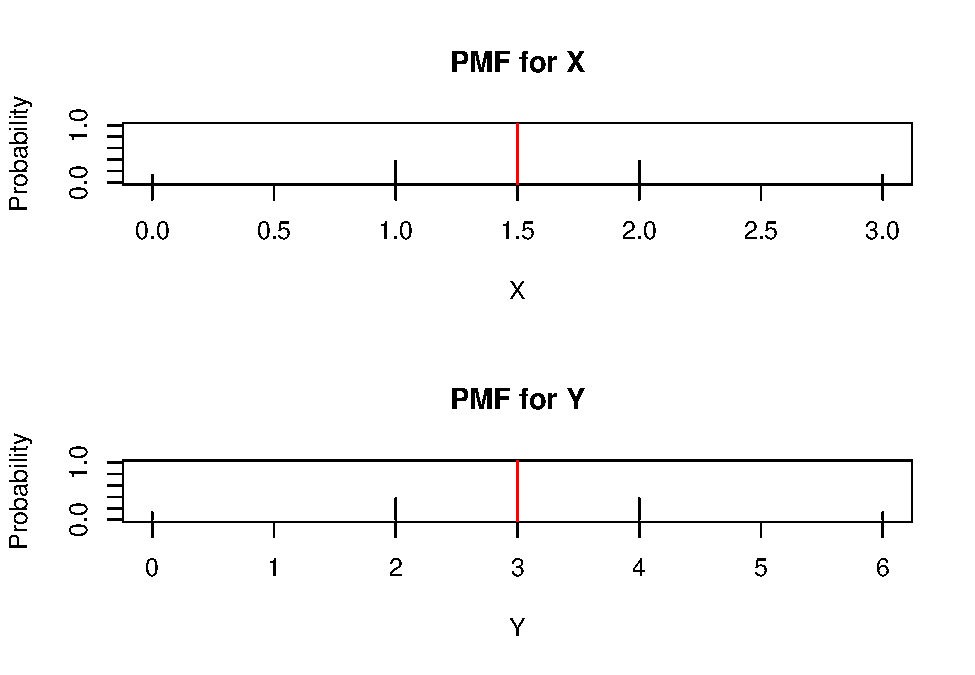
\includegraphics{bookdown-demo_files/figure-latex/3-pmf-lin-1.pdf}
\caption{\label{fig:3-pmf-lin}PMF for X and Y=2X}
\end{figure}

Note that the red vertical lines represent the expected value for the random variable, and since the PMFs are symmetric, the expected value lies right in the middle of the support. Comparing the PMFs in Figure \ref{fig:3-pmf-lin}, we get \(Y\) by multiplying \(X\) by 2. So the support of \(Y\) is now \(\{0,2,4,6\}\) but the associated probabilities are unchanged, so the heights of the probabilities on the vertical axis are unchanged. Therefore, the center, the expected value, is multiplied by the same constant.

Consider another random variable \(W = X+3\). We create the PMF for \(W\) and display it in Figure \ref{fig:3-pmf-lin2} below:

\begin{Shaded}
\begin{Highlighting}[]
\DocumentationTok{\#\#support of X}
\NormalTok{x}\OtherTok{\textless{}{-}}\DecValTok{0}\SpecialCharTok{:}\DecValTok{3}
\DocumentationTok{\#\# PMF for each value in the support. }
\NormalTok{PMFs}\OtherTok{\textless{}{-}}\FunctionTok{c}\NormalTok{(}\DecValTok{1}\SpecialCharTok{/}\DecValTok{8}\NormalTok{, }\DecValTok{3}\SpecialCharTok{/}\DecValTok{8}\NormalTok{, }\DecValTok{3}\SpecialCharTok{/}\DecValTok{8}\NormalTok{, }\DecValTok{1}\SpecialCharTok{/}\DecValTok{8}\NormalTok{)}
\NormalTok{EX}\OtherTok{\textless{}{-}}\FloatTok{1.5}

\DocumentationTok{\#\#support of W}
\NormalTok{w}\OtherTok{\textless{}{-}}\NormalTok{x}\SpecialCharTok{+}\DecValTok{3}
\DocumentationTok{\#\# PMF for each value in the support. }
\NormalTok{PMFs}\OtherTok{\textless{}{-}}\FunctionTok{c}\NormalTok{(}\DecValTok{1}\SpecialCharTok{/}\DecValTok{8}\NormalTok{, }\DecValTok{3}\SpecialCharTok{/}\DecValTok{8}\NormalTok{, }\DecValTok{3}\SpecialCharTok{/}\DecValTok{8}\NormalTok{, }\DecValTok{1}\SpecialCharTok{/}\DecValTok{8}\NormalTok{)}
\NormalTok{EW}\OtherTok{\textless{}{-}}\NormalTok{EX}\SpecialCharTok{+}\DecValTok{3}

\FunctionTok{par}\NormalTok{(}\AttributeTok{mfrow=}\FunctionTok{c}\NormalTok{(}\DecValTok{2}\NormalTok{,}\DecValTok{1}\NormalTok{))}

\DocumentationTok{\#\# create plot of PMF vs each value in support}
\FunctionTok{plot}\NormalTok{(x, PMFs, }\AttributeTok{type=}\StringTok{"h"}\NormalTok{, }\AttributeTok{main =} \StringTok{"PMF for X"}\NormalTok{, }\AttributeTok{xlab=}\StringTok{"X"}\NormalTok{, }\AttributeTok{ylab=}\StringTok{"Probability"}\NormalTok{, }\AttributeTok{ylim=}\FunctionTok{c}\NormalTok{(}\DecValTok{0}\NormalTok{,}\DecValTok{1}\NormalTok{))}
\DocumentationTok{\#\#overlay a line representing EX in red}
\FunctionTok{abline}\NormalTok{(}\AttributeTok{v=}\NormalTok{EX, }\AttributeTok{col=}\StringTok{"red"}\NormalTok{)}

\DocumentationTok{\#\# create plot of PMF vs each value in support}
\FunctionTok{plot}\NormalTok{(w, PMFs, }\AttributeTok{type=}\StringTok{"h"}\NormalTok{, }\AttributeTok{main =} \StringTok{"PMF for w"}\NormalTok{, }\AttributeTok{xlab=}\StringTok{"W"}\NormalTok{, }\AttributeTok{ylab=}\StringTok{"Probability"}\NormalTok{, }\AttributeTok{ylim=}\FunctionTok{c}\NormalTok{(}\DecValTok{0}\NormalTok{,}\DecValTok{1}\NormalTok{))}
\DocumentationTok{\#\#overlay a line representing EW in red}
\FunctionTok{abline}\NormalTok{(}\AttributeTok{v=}\NormalTok{EW, }\AttributeTok{col=}\StringTok{"red"}\NormalTok{)}
\end{Highlighting}
\end{Shaded}

\begin{figure}
\centering
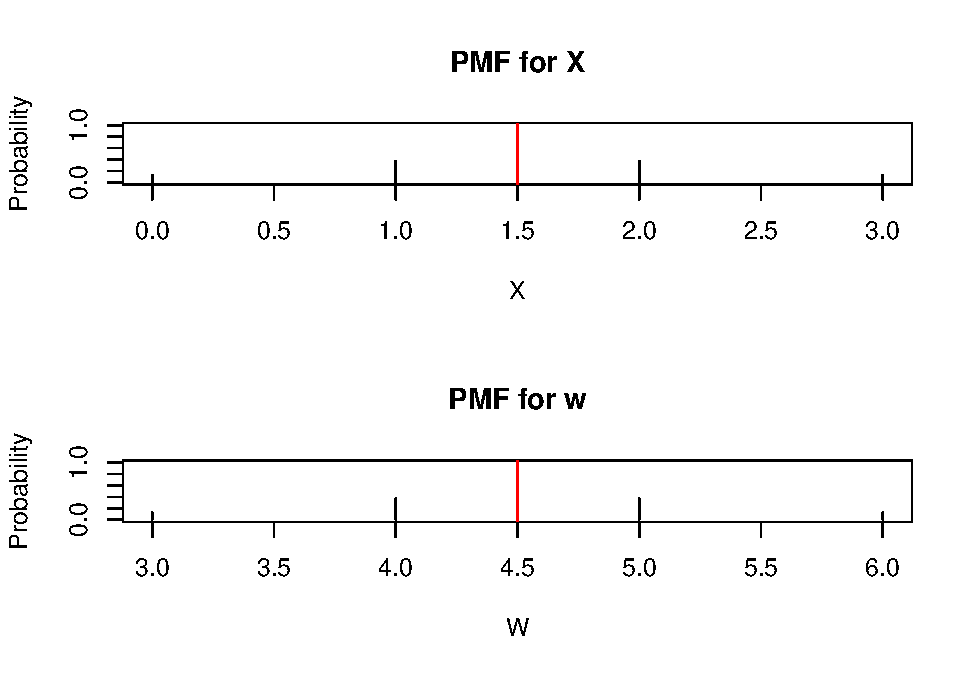
\includegraphics{bookdown-demo_files/figure-latex/3-pmf-lin2-1.pdf}
\caption{\label{fig:3-pmf-lin2}PMF for X and W=X+3}
\end{figure}

Notice the PMFs for \(X\) and \(W\) look almost exactly the same. The only difference is that every value in the support for \(X\) is shifted by 3 units. The probabilities stay the same, so the heights in the PMFs are unchanged. So if every value is shifted by 3 units, the expected value, the long-run average, also gets shifted by 3 units. Adding a constant to a random variable shifts the expected value accordingly.

\subsubsection{One More Example}\label{one-more-example}

We look at one more example to illustrate the usefulness of the linearity of expectations. Consider a drunk man who has to walk on a one-dimensional number line and starts at the 0 position. For each step the drunk man takes, he either moves forward, backward, or stays at the same spot. He steps forward with probability \(p_f\), backward with probability \(p_b\), and stays at the same spot with probability \(p_s\), where \(p_f + p_b+p_s = 1\). Let \(Y\) be the position on the number line of the drunk man after 2 steps. What is the expected position of the drunk man after two steps, i.e.~what is \(E(Y)\)? Assume that each step is independent.

Using brute force, we can find the PMF of \(Y\), and find \(E(Y)\) using equation \eqref{eq:3-EX}. First, we need to find the sample space for \(Y\). With two steps, the sample space is \(\{-2,-1,0,1,2\}\). Next, we need to find the probabilities associated with each outcome in the sample space.

\begin{itemize}
\tightlist
\item
  For \(Y=-2\), the man must move backward on each step. This probability will be \(P(Y=-2) = p_b^2\).
\item
  Likewise, for \(Y=2\), the man must move forward on each step. This probability will be \(P(Y=2) = p_f^2\).
\item
  For \(Y=-1\), the man could stay on the first step, then move back on the second, or move back on the first step, and stay on the second. This probability will be \(P(Y=-1) = p_s p_b + p_b p_s = 2p_b p_s\).
\item
  Likewise, for \(Y=1\), the man could stay on the first step, then move forward on the second, or move forward on the first step, and stay on the second. This probability will be \(P(Y=1) = p_s p_f + p_f p_s = 2p_f p_s\).
\item
  For \(Y=0\), the man could move forward, then backward, or move backward then forward, or stay on both steps. So \(P(Y=0) = p_f p_b + p_b p_f + p_s^2 = p_s^2 + 2 p_b p_f\).
\end{itemize}

Using equation \eqref{eq:3-EX},

\[
\begin{split}
E(Y) &= -2 \times p_b^2 + -1 \times 2p_b p_s + 0 \times p_s^2 + 2 p_b p_f + 1 \times 2p_f p_s + 2 \times p_f^2 \\
       &= 2 (p_f - p_b)
\end{split}
\]

Note: I skipped a lot of messy algebra to get to the end result. Even with skipping some of the messy algebra, setting up the PMF was quite a bit of work.

Suppose we use the linearity of expectations in equation \eqref{eq:3-linEX}. Let \(Y_1, Y_2\) denote the distance the man moves at step 1 and 2 respectively. Then \(Y = Y_1 + Y_2\). The sample of \(Y_1\) and \(Y_2\) are the same: \(\{-1,0,1\}\). Both \(Y_1\) and \(Y_2\) have the following PMF:

\begin{itemize}
\tightlist
\item
  \(P(Y_i = -1) = p_b\)
\item
  \(P(Y_i = 0) = p_s\)
\item
  \(P(Y_i = 1) = p_f\)
\end{itemize}

And using equation \eqref{eq:3-EX},

\[
\begin{split}
E(Y_i) &= -1 \times p_b + 0 \times p_s + 1 \times p_f \\
       &= p_f - p_b
\end{split}
\]

So therefore \(E(Y) = E(Y_1 + Y_2) = E(Y_1) + E(Y_2) = 2(p_f - p_b)\). Both approaches resulted in the same answer, but notice how much simpler its was to obtain the solution using linearity of expectations. Imagine if we wanted to find the expected position after 500 steps? Writing out the sample space for 500 steps will be extremely long.

View the video below for a more detailed explanation of this worked example:

\subsection{Law of the Unconscious Statistician}\label{law-of-the-unconscious-statistician}

Suppose we have the PMF of a random variable \(X\), and we want to find \(E(g(X))\), where \(g\) is a function of \(X\) (you can think of \(g\) as a transformation performed on \(X\)). One idea could be to find the PMF of \(g(X)\) and then use the definition of expectation in equation \eqref{eq:3-EX}. But we have seen in the previous subsection that finding the sample space after transforming the random variable can be challenging. It turns out we can find \(E(g(X))\) based on the PMF of \(X\), without having to find the PMF of \(g(X)\).

This is done through the \textbf{Law of the Unconscious Statistician (LOTUS)}. Let \(X\) be a discrete random variable with support \(\{x_1, x_2, \cdots \}\), and \(g\) is a function applied to \(X\), then

\begin{equation} 
E(g(X)) = \sum_{i=j}^{\infty} g(x_j) P(X=x_j).
\label{eq:3-lotus}
\end{equation}

An application of LOTUS is in finding the variance of a discrete random variable.

\subsection{Variance}\label{variance}

We have talked about the shape of the distribution of a discrete random variable, and its expected value. One more measure that we are interested in is the spread associated with the distribution. One common measure is the variance of the random variable.

The \textbf{variance} of a random variable \(X\) is

\begin{equation} 
Var(X) = E[(X - EX)^2]
\label{eq:3-var2}
\end{equation}

and the \textbf{standard deviation} of a random variable \(X\) is the squareroot of its variance

\begin{equation} 
SD(X) = \sqrt{Var(X)}.
\label{eq:3-sd}
\end{equation}

Looking at equation \eqref{eq:3-var2} a little more closely, we can see a natural interpretation of the variance of a random variable: it is the average squared distance of the random variable from its mean, in the long-run. An equivalent formula for the variance of a random variable is

\begin{equation} 
Var(X) = E(X^2) - (EX)^2.
\label{eq:3-var}
\end{equation}

Equation \eqref{eq:3-var} is easier to work with than equation \eqref{eq:3-var2} when performing actual calculations.

Let us now go back to our original example, where \(X\) denotes the number of heads out of 3 coin flips. Earlier, we found the PMF of this random variable, per Table \ref{tab:3-pmf-tab}, and we found its expectation to be 1.5. To find the variance of \(X\) using equation \eqref{eq:3-var}, we find \(E(X^2)\) first using LOTUS in equation \eqref{eq:3-lotus}

\[
\begin{split}
E(X^2) &= 0^2 \times \frac{1}{8} + 1^2 \times \frac{3}{8} + 2^2 \times \frac{3}{8} + 3^2 \times \frac{1}{8} \\
       &= 3
\end{split}
\]

so \(Var(x) = 3 - 1.5^2 = \frac{3}{4}\).

\emph{Thought question}: Try to find \(Var(X)\) using equation \eqref{eq:3-var2} and LOTUS. You should arrive at the same answer but the steps may be a bit more complicated.

View the video below for a more detailed explanation on how to calculate variance of discrete random variables using equations \eqref{eq:3-var} and \eqref{eq:3-var2}:

\subsubsection{Properties of Variance}\label{var-prop}

Variance has the following properties:

\begin{itemize}
\tightlist
\item
  \(Var(X+c) = Var(X)\), where \(c\) is a constant. This should make sense, since if we add a constant to a random variable, we shift it by \(c\) units. As shown earlier in Figure \ref{fig:3-pmf-lin2}, the expected value also gets shifted by \(c\) units. Variance measures the average squared distance of a variable from its mean. So the distance, and the squared distance, of \(X\) from its mean is unchanged.
\item
  \(Var(cX) = c^2 Var(X)\). Look at Figure \ref{fig:3-pmf-lin}, notice the distance between each value in the support from its expected value gets multiplied by 2 (since \(Y=2X\)). So if we multiply a random variable by \(c\), the distance between each value in the support on its expected value is multiplied by \(c\). Since variance measures squared distance, the variance gets multiplied by \(c^2\).
\item
  If \(X\) and \(Y\) are independent random variables, then \(Var(X+Y) = Var(X) + Var(Y)\).
\end{itemize}

\section{Common Discrete Random Variables}\label{common-discrete-random-variables}

Next, we will introduce some commonly used distributions that may be used for discrete random variables. A number of common statistical models (for example, logistic regression, Poisson regression) are based on these distributions.

\subsection{Bernoulli}\label{bernoulli}

The Bernoulli distribution might be the simplest discrete random variable. The support for such a random variable is \(\{0,1\}\). In other words, the value of a random variable that follows a Bernoulli distribution is either 0 or 1. A Bernoulli distribution is also described by the parameter \(p\), which is the probability that the random variable takes on the value of 1.

More formally, a random variable \(X\) follows a \textbf{Bernoulli distribution} with parameter \(p\) if \(P(X=1) = p\) and \(P(X=0) = 1-p\), where \(0<p<1\). Using mathematical notation, we can write \(X \sim Bern(p)\) to express that the random variable \(X\) is distributed as a Bernoulli with parameter \(p\). The PMF of a Bernoulli distribution is written as

\begin{equation} 
P(X=k) = p^k (1-p)^{1-k}
\label{eq:3-bern}
\end{equation}

for \(k=0, 1\).

It is not enough to specify that a random variable follows a Bernoulli distribution. We need to also clearly specify the value of the parameter \(p\). Consider the following two examples which describe two different experiments:

\begin{itemize}
\item
  Suppose I flip a fair coin once. Let \(Y=1\) if the coin lands heads, and \(Y=0\) if the coin lands tails. \(Y \sim Bern(\frac{1}{2})\) in this example since the coin is fair.
\item
  Suppose I am asked a question and I am given 5 multiple choices, of which only 1 is the correct answer. I have no idea about the topic, and the multiple choices do not help, so I have to guess. Let \(W=1\) if I answer correctly, and \(W=0\) if I answer incorrectly. \(W \sim Bern(\frac{1}{5})\).
\end{itemize}

\(P(Y=1)\) and \(P(W=1)\) are not the same in these examples.

Fairly often, when we have a Bernoulli random variable, the event that results in the random variable being coded as 1 is called a \textbf{success}, and the event that results in the random variable being coded as 0 is called a \textbf{failure}. In such a setting, the parameter \(p\) is called the \textbf{success probability} of the Bernoulli distribution. An experiment that has a Bernoulli distribution can be called a Bernoulli trial.

If you go back to the second example in section \ref{eg2}, we were modeling whether a job applicant receives a callback or not. In this example, we could let \(V\) be the random variable that an applicant receives a callback, with \(V=1\) denoting the applicant received a callback, and \(V=0\) when the applicant did not receive a callback. We used logistic regression in the example. It turns out that logistic regression is used when the variable of interest follows a Bernoulli distribution.

\subsubsection{Properties of Bernoulli}\label{properties-of-bernoulli}

Consider \(X\) is a Bernoulli distribution with parameter \(p\). The expectation of a Bernoulli distribution is

\begin{equation} 
E(X) = p
\label{eq:3-bern-EX}
\end{equation}

and its variance is

\begin{equation} 
Var(X) = p(1-p).
\label{eq:3-bern-var}
\end{equation}

\emph{Thought question}: Use the definition of expectations for discrete random variables, equation \eqref{eq:3-EX}, and the PMF of a Bernoulli random variable, and LOTUS to prove equations \eqref{eq:3-bern-EX} and \eqref{eq:3-bern-var}.

The expected value being equal to \(p\) for a Bernoulli distribution should make sense. Remember that the support for such a random variable is 0 or 1, with \(P(X=1) = p\). Using the frequentist viewpoint, if we were to flip a coin and record heads or tails, and repeat this coin flipping many times, we will have record a bunch of 0s and 1s to represent the result for all the coin flips. The average of this bunch of 0s and 1s is just the proportion of 1s.

The equation for the variance of a Bernoulli distribution exhibits an interesting and intuitive behavior. Figure \ref{fig:3-varBern} below shows how the variance behaves as we vary the value of \(p\):

\begin{Shaded}
\begin{Highlighting}[]
\NormalTok{p}\OtherTok{\textless{}{-}}\FunctionTok{seq}\NormalTok{(}\DecValTok{0}\NormalTok{,}\DecValTok{1}\NormalTok{,}\AttributeTok{by =} \FloatTok{0.001}\NormalTok{) }\DocumentationTok{\#\#sequence of values for p}
\NormalTok{Bern\_var}\OtherTok{\textless{}{-}}\NormalTok{p}\SpecialCharTok{*}\NormalTok{(}\DecValTok{1}\SpecialCharTok{{-}}\NormalTok{p) }\DocumentationTok{\#\#variance of Bernoulli}
\DocumentationTok{\#\#plot variance against p}
\FunctionTok{plot}\NormalTok{(p, Bern\_var, }\AttributeTok{ylab=}\StringTok{"Variance"}\NormalTok{, }\AttributeTok{main=}\StringTok{"Variance of Bernoulli as p is Varied"}\NormalTok{)}
\end{Highlighting}
\end{Shaded}

\begin{figure}
\centering
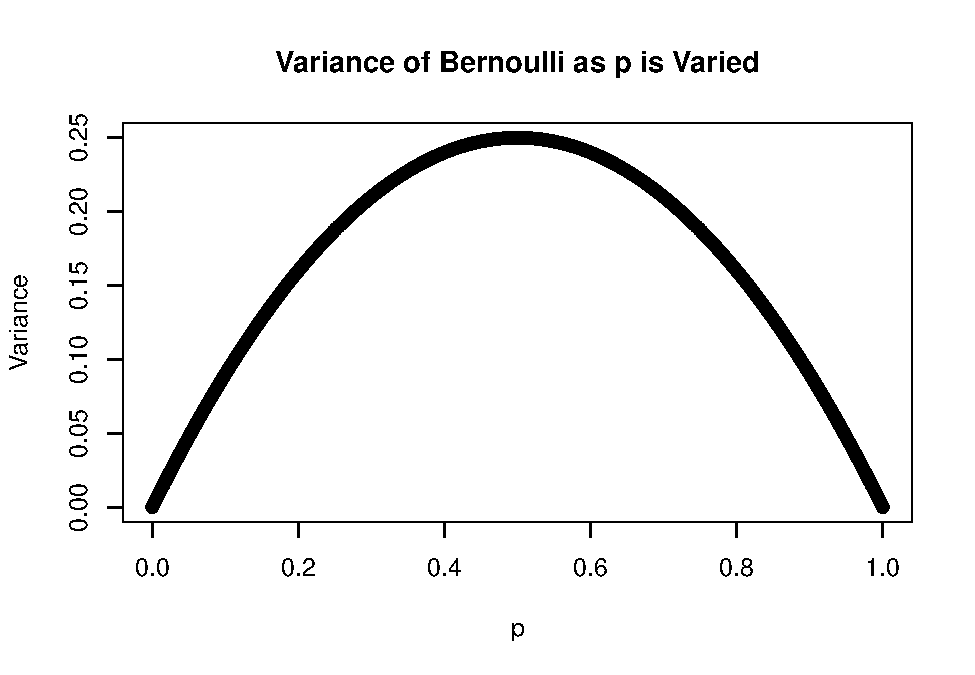
\includegraphics{bookdown-demo_files/figure-latex/3-varBern-1.pdf}
\caption{\label{fig:3-varBern}Variance of Bernoulli}
\end{figure}

Notice the variance is at a maximum when \(p=0.5\), and the variance is minimum (in fact it is 0) when \(p=0\) or \(p=1\). If we have a biased coin such that it always lands heads, every coin flip will land on heads with no exception. There is no variability in the result, and we have utmost certainty in the result of each coin flip. On the other hand, if the coin is fair such that \(p=0.5\), we have the least certainty in the result of each coin flip, and so variance is maximum when the coin is fair.

Another application of this property is during election results (assuming 2 candidates, but the same idea applies for more candidates). For swing states where the race is closer (so \(p\) is closer to half), projections on the winner have more uncertainty and so we need to get more data and wait longer for the projections. For states that primarily vote for one candidate (so \(p\) is closer to 0 or 1), projections happen a lot quicker as projections have less uncertainty.

\subsection{Binomial}\label{binomial}

Suppose we have an experiment that follows a Bernoulli distribution, and we perform this experiment \(n\) times (sometimes called trials), each time with the same success probability \(p\). The experiments are independent from each other. Let \(X\) denote the number of successes out of the \(n\) trials. \(X\) follows a \textbf{binomial distribution} with parameters \(n\) and \(p\) (number of trials and success probability). We write \(X \sim Bin(n,p)\) to express that \(X\) follows a binomial distribution with parameters \(n\) and \(p\), with \(n>0\) and \(0<p<1\). The PMF of a Binomial distribution is written as

\begin{equation} 
P(X=k) = \binom{n}{k} p^k (1-p)^{n-k}
\label{eq:3-bin}
\end{equation}

for \(k=0,1,2, \cdots, n\), which is also the support of the binomial distribution.

In equation \eqref{eq:3-bin}, \(\binom{n}{k}\) is called the binomial coefficient, and it is the number of combinations that result in \(k\) successes out of the \(n\) trials. The binomial coefficient can be found using

\begin{equation} 
\binom{n}{k} =  \frac{n!}{k! (n-k)!}.
\label{eq:3-bincoeff}
\end{equation}

\(n!\) is called n-factorial, and is the product of all positive integers less than or equal to n.~So \(n! = n \times (n-1) \times (n-2) \times \cdots \times 1.\) As an example \(5! = 5 \times 4 \times 3 \times 2 \times 1 = 120\), or using R:

\begin{Shaded}
\begin{Highlighting}[]
\FunctionTok{factorial}\NormalTok{(}\DecValTok{5}\NormalTok{)}
\end{Highlighting}
\end{Shaded}

\begin{verbatim}
## [1] 120
\end{verbatim}

Note: A fairly common model, the logistic regression model with aggregated data, is based on the binomial distribution. We mentioned logistic regression earlier. The difference between these two (with and without aggregated data) is based on the structure of the data frame. If you are interested in these differences, please read \url{https://www.r-bloggers.com/2021/02/how-to-run-logistic-regression-on-aggregate-data-in-r/}.

We go back to our first example of counting the number of heads out of three coin flips follows a binomial distribution.

\begin{itemize}
\tightlist
\item
  Each coin flip is either heads or tails. There are only two outcomes for each flip.
\item
  The success probability, the probability of heads, is 0.5 and is the same for each flip. The parameter is fixed for each flip.
\item
  The result of each flip is independent of other flips since other flips do not affect the outcome.
\item
  The number of trials (flips in this example) is \(n=3\) is specified as a fixed value.
\end{itemize}

Since these four conditions are met, the number of heads in 3 coin flips can be modeled using a binomial distribution. We let \(x\) denote the number of heads in 3 coin clips, so we write \(X \sim Bin(3,0.5)\).

Suppose we want to calculate \(P(X=2)\) using equation \eqref{eq:3-bin}:

\[
\begin{split}
P(X=2) &= \binom{3}{2} (0.5)^2 (0.5)^1\\
       &= \frac{3!}{2! 1!} (0.5)^2 (0.5)^1 \\
       &= 3 \times \frac{1}{8} \\
       &= \frac{3}{8}.
\end{split}
\]

In this example, the binomial coefficient equals to 3. Which indicates there were 3 combinations to obtain 2 heads in 3 coin flips. \(P(X=2)\) can be written as \(P(HHT \cup HTH \cup THH)\). Solving for \(P(HHT \cup HTH \cup THH)\), we have

\[
\begin{split}
P(HHT \cup HTH \cup THH) &= P(HHT) + P(HTH) + P(THH)\\
       &= 0.5^3 + 0.5^3 + 0.5^3 \\
       &= 3 \times \frac{1}{8} \\
       &= \frac{3}{8}.
\end{split}
\]
so we could have solved this using basic probability rules from the previous module, without using the PMF of the binomial distribution in equation \eqref{eq:3-bin}. Of course, the PMF of the binomial distribution gets a lot more convenient if \(n\) gets larger, as the number of combinations and sample space get a lot larger.

We can also use R to find \(P(X=2)\):

\begin{Shaded}
\begin{Highlighting}[]
\FunctionTok{dbinom}\NormalTok{(}\DecValTok{2}\NormalTok{,}\DecValTok{3}\NormalTok{,}\FloatTok{0.5}\NormalTok{) }\DocumentationTok{\#\#specify values of k, n, p in this order}
\end{Highlighting}
\end{Shaded}

\begin{verbatim}
## [1] 0.375
\end{verbatim}

\subsubsection{Relationship Between Binomial and Bernoulli}\label{relationship-between-binomial-and-bernoulli}

Looking at the description of the Bernoulli and binomial distributions, you may notice that a Bernoulli random variable is a special case of a binomial random variable when \(n=1\), i.e.~when we have only 1 trial.

The binomial random variable is also sometimes viewed as the sum of \(n\) independent Bernoulli random variables, all with the same value of \(p\).

\subsubsection{Properties of Binomial}\label{properties-of-binomial}

If \(X \sim Bin(n,p)\), then

\begin{equation} 
E(X) = np
\label{eq:3-bin-EX}
\end{equation}

and

\begin{equation} 
Var(X) = np(1-p).
\label{eq:3-bin-var}
\end{equation}

These results should make sense when we note the relationship between a binomial random variable and Bernoulli random variable. Suppose we have random variables \(Y_1, Y_2, \cdots, Y_n\) and they are all Bernoulli random variables with parameter \(p\) and are independent. Then \(Y = Y_1 + Y_2 + \cdots + Y_n \sim Bin(n,p)\). Therefore, using the linearity of expectations in equation \eqref{eq:3-linEX}, \(E(Y) = E(Y_1) + E(Y_2) + \cdots + E(Y_n) = np\). Since \(Y_1, Y_2, \cdots, Y_n\) are independent, \(Var(Y) = Var(Y_1) + Var(Y_2) + \cdots + Var(Y_n) = np(1-p)\).

\subsubsection{PMFs of Binomial}\label{pmfs-of-binomial}

We take a look at the PMFs of a few binomials, all with \(n=10\) but we vary \(p\) to be 0.2, 0.5, and 0.9, in Figure \ref{fig:3-pmfs}:

\begin{figure}
\centering
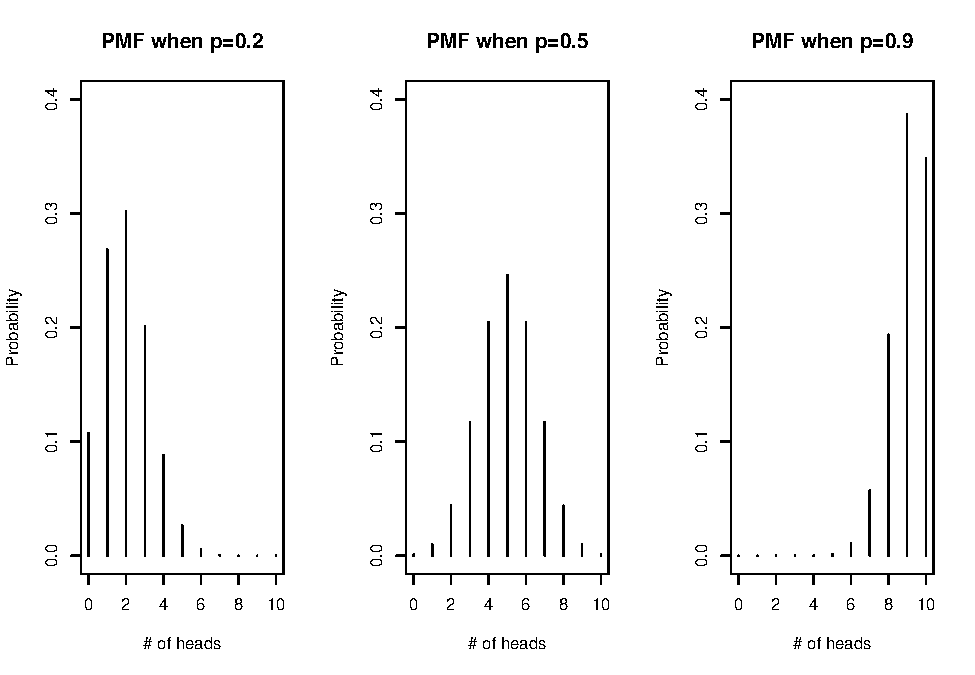
\includegraphics{bookdown-demo_files/figure-latex/3-pmfs-1.pdf}
\caption{\label{fig:3-pmfs}PMF for X, n=10, p varied}
\end{figure}

From figure \ref{fig:3-pmfs}, we can see that the distribution of the binomial is symmetric when \(p=0.5\), as middle values of \(k\) have higher probabilities, and the probabilities decrease as we go further away from the middle. When \(p \neq 0.5\), we see that the distribution gets skewed. When the success probability is small, smaller number of successes are likelier, and when the success probability is large, larger number of successes are likelier, which is intuitive. If the probability of success is small, we expect most outcomes to be failures.

\subsection{Poisson}\label{poisson}

One more common distribution used for discrete random variables is the Poisson distribution. This is often used when the variable of interest is what we call count data (the support is non negative integers), for example, the number of cars that cross an intersection during the day.

A random variable \(X\) follows a \textbf{Poisson distribution} with parameter \(\lambda\), where \(\lambda>0\). Using mathematical notation, we can write \(X \sim Pois(\lambda)\) to express that the random variable \(X\) is distributed as a Poisson with parameter \(p\). The PMF of a Poisson distribution is written as

\begin{equation} 
P(X=k) = \frac{e^{-\lambda}\lambda^k}{k!} 
\label{eq:3-pois}
\end{equation}

for \(k=0,1,2,\cdots\). \(\lambda\) is sometimes called a rate parameter, as it is related to the rate of arrivals, for example, the number of that cross an intersection during a period of time.

\subsubsection{Properties of Poisson}\label{properties-of-poisson}

If \(X \sim Pois(\lambda)\), then

\begin{equation} 
E(X) = \lambda
\label{eq:3-pois-EX}
\end{equation}

and

\begin{equation} 
Var(X) = \lambda.
\label{eq:3-pois-var}
\end{equation}

These imply that larger values of a Poisson random variable are associated with larger variances. This is a common feature for count data. Consider the number of cars that cross an intersection during a one-hour time period. Consider the average number of cars during rush hour, say between 5 and 6pm. This average number is large, but the number could be a lot smaller due to inclement weather, or the number could get a lot larger is there is a convention occurring nearby. On the other hand, consider the average number of cars between 3 and 4am. This average number is small, and is likely to be small all the time, regardless of weather conditions and whether special events are happening.

Another interesting property of the Poisson distribution is that it is skewed when \(\lambda\) is small, and approaches a bell-shaped distribution as \(\lambda\) gets bigger. Figure \ref{fig:3-pmfs-lambda} displays density plots of Poisson distributions as \(\lambda\) is varied:

\begin{Shaded}
\begin{Highlighting}[]
\DocumentationTok{\#\#calculate probability of Poisson with these values on the support}
\NormalTok{x}\OtherTok{\textless{}{-}}\DecValTok{0}\SpecialCharTok{:}\DecValTok{20}
\NormalTok{lambda}\OtherTok{\textless{}{-}}\FunctionTok{c}\NormalTok{(}\FloatTok{0.5}\NormalTok{, }\DecValTok{1}\NormalTok{, }\DecValTok{4}\NormalTok{, }\DecValTok{10}\NormalTok{) }\DocumentationTok{\#\#try 4 different values of lambda}

\DocumentationTok{\#\#create PMFs of these 4 Poissons with different lambdas}
\FunctionTok{par}\NormalTok{(}\AttributeTok{mfrow=}\FunctionTok{c}\NormalTok{(}\DecValTok{2}\NormalTok{,}\DecValTok{2}\NormalTok{))}
\ControlFlowTok{for}\NormalTok{ (i }\ControlFlowTok{in} \DecValTok{1}\SpecialCharTok{:}\DecValTok{4}\NormalTok{)}
  
\NormalTok{\{}
\NormalTok{  dens}\OtherTok{\textless{}{-}}\FunctionTok{dpois}\NormalTok{(x,lambda[i])}
  \FunctionTok{plot}\NormalTok{(x, dens, }\AttributeTok{type=}\StringTok{"l"}\NormalTok{, }\AttributeTok{main=}\FunctionTok{paste}\NormalTok{(}\StringTok{"Lambda is"}\NormalTok{, lambda[i]))}
\NormalTok{\}}
\end{Highlighting}
\end{Shaded}

\begin{figure}
\centering
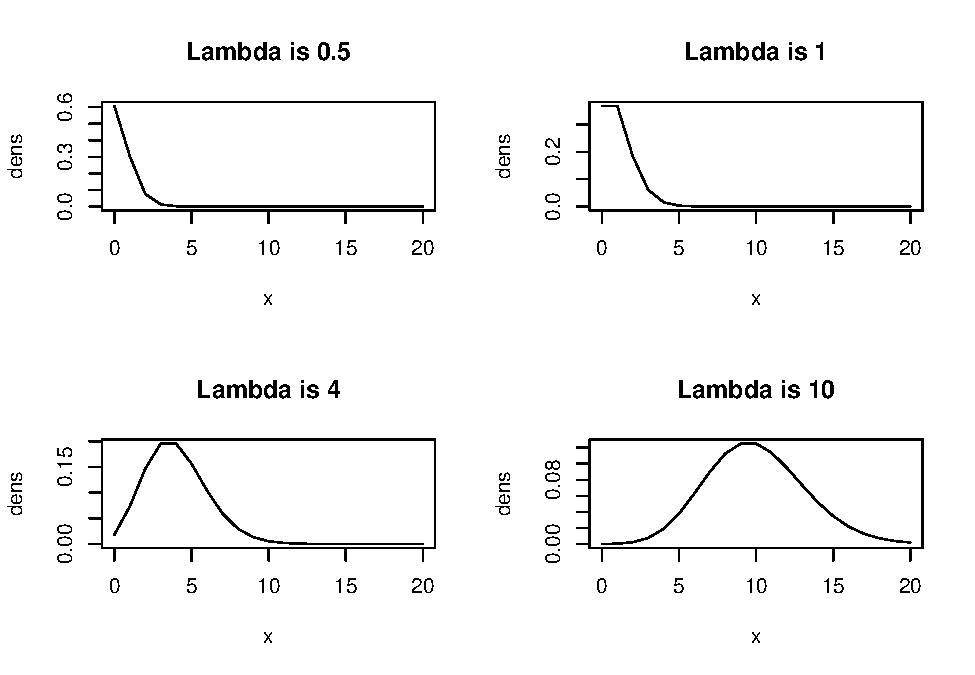
\includegraphics{bookdown-demo_files/figure-latex/3-pmfs-lambda-1.pdf}
\caption{\label{fig:3-pmfs-lambda}PMF for Poissons as Rate Parameter is Varied}
\end{figure}

\subsubsection{Poisson Approximation to Binomial}\label{poisson-approximation-to-binomial}

If \(X \sim Bin(n,p)\), and if \(n\) is large and \(p\) is small, then the PMF of \(X\) can be approximated by a Poisson distribution with rate parameter \(\lambda = np\). In other words, the approximation works better as \(n\) gets larger and \(np\) gets smaller.

There are several rules of thumbs that exist to guide as to how large \(n\) should be and how small \(np\) should be. The National Institute of Standards and Technology \href{https://www.itl.nist.gov/div898/handbook/pmc/section3/pmc331.htm}{(NIST)} suggest \(n \geq 20\) and \(p \leq 0.05\), or \(n \geq 100\), and \(np \leq 10\).

One of the main for using this approximation, instead of directly using the binomial distribution, is that the binomial coefficient can become computationally expensive to compute when \(n\) is large.

Consider this example: A company manufactures computer chips, and 2 percent of chips are defective. The quality control manager randomly samples 100 chips coming off the assembly line. What is the probability that at most 3 chips are defective?

Let \(Y\) denote the number of chips that are defective out of 100 chips.

\begin{itemize}
\tightlist
\item
  Each chip is either defective or not. There are only two outcomes for each chip.
\item
  The ``success'' probability is 0.02 for each chip. This probability is assumed to be fixed for each chip.
\item
  We have to assume that each chip is independent.
\item
  The number of chips is fixed at \(n=100\).
\end{itemize}

So we can model \(Y \sim Bin(100,0.02)\), as long as we assume the chips the independent. To find \(P(Y \leq 3)\), we can:

\begin{itemize}
\tightlist
\item
  use the binomial distribution, or
\item
  approximate it using \(Pois(2)\), as \(\lambda = np = 100 \times 0.02\).
\end{itemize}

\begin{Shaded}
\begin{Highlighting}[]
\DocumentationTok{\#\#set up binomial}
\NormalTok{n}\OtherTok{\textless{}{-}}\DecValTok{100} 
\NormalTok{p}\OtherTok{\textless{}{-}}\FloatTok{0.02} 
\NormalTok{y}\OtherTok{\textless{}{-}}\DecValTok{0}\SpecialCharTok{:}\DecValTok{3} \DocumentationTok{\#\#we want P(Y=0), P(Y=1), P(Y=2), P(Y=3)}
\FunctionTok{sum}\NormalTok{(}\FunctionTok{dbinom}\NormalTok{(y,n,p))}
\end{Highlighting}
\end{Shaded}

\begin{verbatim}
## [1] 0.8589616
\end{verbatim}

\begin{Shaded}
\begin{Highlighting}[]
\DocumentationTok{\#\#Use Poisson to approx binomial}
\NormalTok{lambda}\OtherTok{\textless{}{-}}\NormalTok{n}\SpecialCharTok{*}\NormalTok{p}
\FunctionTok{sum}\NormalTok{(}\FunctionTok{dpois}\NormalTok{(y,lambda))}
\end{Highlighting}
\end{Shaded}

\begin{verbatim}
## [1] 0.8571235
\end{verbatim}

Notice the values are very close to each other.

\section{Using R}\label{Rdis}

R has built in functions to compute the PMF, CDF, percentiles, as well as simulate data of common distributions. We will start using a random variable \(Y\) which follows binomial distribution, with \(n=5, p = 0.3\) as an example first. Note in this example that the support for \(Y\) is \(\{0,1,2,3,4,5 \}\).

\begin{enumerate}
\def\labelenumi{\arabic{enumi}.}
\tightlist
\item
  To find \(P(Y=2)\), use:
\end{enumerate}

\begin{Shaded}
\begin{Highlighting}[]
\FunctionTok{dbinom}\NormalTok{(}\DecValTok{2}\NormalTok{, }\DecValTok{5}\NormalTok{, }\FloatTok{0.3}\NormalTok{) }\DocumentationTok{\#\#supply the value of Y you want, then the parameters n and p in this order}
\end{Highlighting}
\end{Shaded}

\begin{verbatim}
## [1] 0.3087
\end{verbatim}

The probability that \(Y\) is equal to 2 is 0.3087.

\begin{enumerate}
\def\labelenumi{\arabic{enumi}.}
\setcounter{enumi}{1}
\tightlist
\item
  To find \(P(Y \leq 2)\), use:
\end{enumerate}

\begin{Shaded}
\begin{Highlighting}[]
\FunctionTok{pbinom}\NormalTok{(}\DecValTok{2}\NormalTok{, }\DecValTok{5}\NormalTok{, }\FloatTok{0.3}\NormalTok{) }\DocumentationTok{\#\#supply the value of Y you want, then the parameters n and p in this order}
\end{Highlighting}
\end{Shaded}

\begin{verbatim}
## [1] 0.83692
\end{verbatim}

The probability that \(Y\) is less than or equal to 2 is 0.83692.

\begin{enumerate}
\def\labelenumi{\arabic{enumi}.}
\setcounter{enumi}{2}
\tightlist
\item
  To find the value on the support that corresponds to the median (or 50th percentile), use:
\end{enumerate}

\begin{Shaded}
\begin{Highlighting}[]
\FunctionTok{qbinom}\NormalTok{(}\FloatTok{0.5}\NormalTok{, }\DecValTok{5}\NormalTok{, }\FloatTok{0.3}\NormalTok{) }\DocumentationTok{\#\#supply the value of the percentile you need, then the parameters n and p in this order}
\end{Highlighting}
\end{Shaded}

\begin{verbatim}
## [1] 1
\end{verbatim}

The median of a binomial distribution with 5 trials and success probability 0.3 is 1.

\begin{enumerate}
\def\labelenumi{\arabic{enumi}.}
\setcounter{enumi}{3}
\tightlist
\item
  To simulate 10 realizations (replications) of \(Y\), use:
\end{enumerate}

\begin{Shaded}
\begin{Highlighting}[]
\FunctionTok{set.seed}\NormalTok{(}\DecValTok{2}\NormalTok{) }\DocumentationTok{\#\#use set.seed() so we get the same random numbers each time the code is run}
\FunctionTok{rbinom}\NormalTok{(}\DecValTok{10}\NormalTok{, }\DecValTok{5}\NormalTok{, }\FloatTok{0.3}\NormalTok{) }\DocumentationTok{\#\#supply the number of simulated data you need, then the parameters n and p}
\end{Highlighting}
\end{Shaded}

\begin{verbatim}
##  [1] 1 2 2 0 3 3 0 2 1 2
\end{verbatim}

This outputs a vector of length 10. Each value represents the result of each rep. So the first time we ran the binomial distribution with \(n=5, p=0.3\), only 1 out of the 5 was a success. The second time it was run, only 2 out of the 5 was a success, and so on.

Notice these functions all ended with \texttt{binom}. We just added a different letter first, depending on whether we want the PMF, CDF, percentile, or random draw. The letters are \texttt{d}, \texttt{p}, \texttt{q}, and \texttt{r} respectively.

The same idea works for any other distribution. For example, to find the probability of a Poisson distribution with rate parameter 2 being equal to 1, we type:

\begin{Shaded}
\begin{Highlighting}[]
\FunctionTok{dpois}\NormalTok{(}\DecValTok{1}\NormalTok{, }\DecValTok{2}\NormalTok{) }\DocumentationTok{\#\#supply value of k, then parameter}
\end{Highlighting}
\end{Shaded}

\begin{verbatim}
## [1] 0.2706706
\end{verbatim}

\emph{Thought questions:} Suppose \(Y \sim Pois(1)\).

\begin{itemize}
\tightlist
\item
  Find \(P(Y \leq 2)\).
\item
  Find the 75th percentile of \(Y\).
\item
  Simulate 10,000 reps from Y, and find its sample mean. Is the sample mean close to the expected value?
\end{itemize}

\chapter{Continuous Random Variables}\label{continuous-random-variables}

This module is based on Introduction to Probability (Blitzstein, Hwang), Chapters 5 and 6. You can access the book for free at \url{https://stat110.hsites.harvard.edu/} (and then click on Book). Please note that I cover additional topics, and skip certain topics from the book. You may skip Examples 5.1.6, 5.1.7, Proposition 5.2.3, Example 5.2.4, Sections 5.2.6, 5.2.7, Definition 5.3.7, Theorem 5.3.8, Example 5.4.7, Sections 5.5, 5.6, 5.7, Proposition 6.2.5, 6.2.6, Theorem 6.3.4, Sections 6.4 to 6.7 from the book.

\section{Introduction}\label{introduction}

In the previous module, we learned about discrete random variables. We learned how their distributions can be described by the PMFs and CDFs, how to find their expected values and variances, as well as common distributions for discrete random variables. We will learn about their counterparts when dealing with continuous random variables. The concepts are similar, but how they are computed can be quite different.

As a reminder:

\begin{itemize}
\tightlist
\item
  A \textbf{discrete random variable} can only take on a countable (finite or infinite) number of values.
\item
  A \textbf{continuous random variable} can take on an uncountable number of values in an interval of real numbers.
\end{itemize}

For example, height of an American adult is a continuous random variable, as height can take on any value in interval between 40 and 100 inches. All values between 40 and 100 are possible. We cannot list all possible real numbers in this range as the list is never ending.

The sample space associated with a continuous random variable will be difficult to list, since it takes on an uncountable number of values. Using the example of heights of American adults, any real number between 40 and 100 inches is possible.

This is different from a discrete random variable where we would list the sample space, or support, and then find the probability associated with each value in the support.

Similar to discrete random variables, we want to describe the shape of the distribution, the centrality, and the spread of a continuous random distribution so we have an idea of probabilities associated with different ranges of values of the random variable.

\section{Cumulative Distribution Functions (CDFs)}\label{cumulative-distribution-functions-cdfs-1}

We start by talking about the cumulative distribution function, as its definition applies to both discrete and continuous random variables. The CDF of a random variable \(X\) is \(F_X(x) = P(X \leq x)\). The difference lies in how a CDF looks visually.

Take a look at the CDF of a discrete random variable and the CDF of a continuous random variable below in Figure \ref{fig:4-compare}:

\begin{figure}
\centering
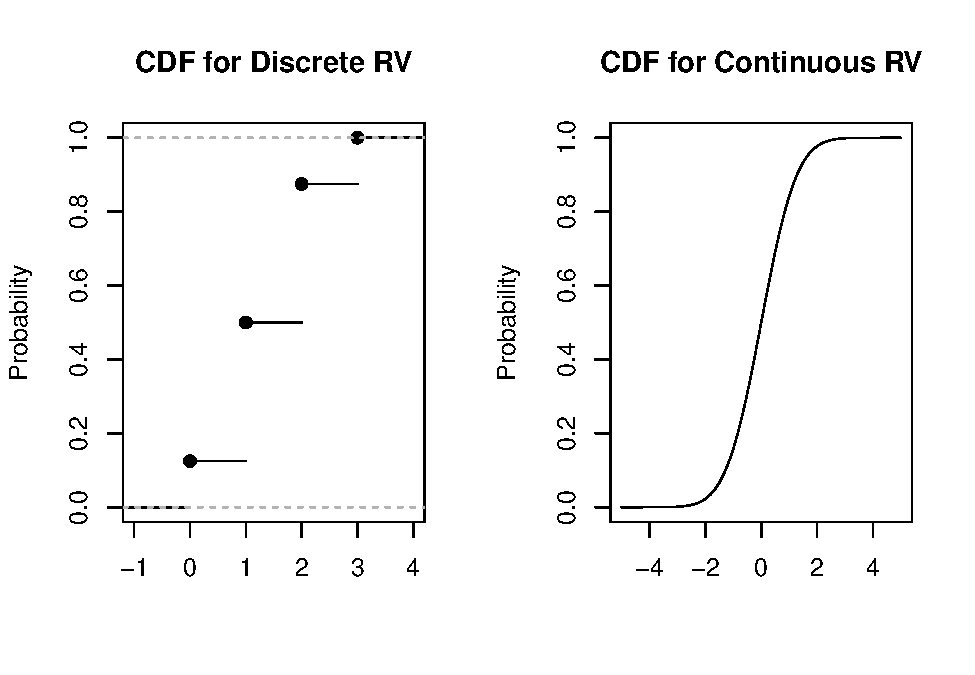
\includegraphics{bookdown-demo_files/figure-latex/4-compare-1.pdf}
\caption{\label{fig:4-compare}CDF for Discrete RV vs CDF for Continuous RV}
\end{figure}

As mentioned in the previous module, the CDF for a discrete random variable is what is called a step function, as it jumps at each value of the support. On the other hand, the CDF for a continuous random variable increases smoothly as its sample space is infinite.

The height of the CDF informs us the percentile associated with the value of the random variable. Looking at the CDF for the continuous random variable in Figure \ref{fig:4-compare}, the height is 0.5 when the random variable is 0, so a value of 0 corresponds to the 50th percentile of this distribution.

The technical definition of a continuous random variable is: A random variable has a continuous distribution if its CDF is differentiable.

A discrete random variable fails in this definition since its derivative is undefined at the jumps.

\subsection{Valid CDFs}\label{valid-cdfs-1}

The criteria for a valid CDF is the same, it does not matter if the random variable is discrete or continuous:

\begin{itemize}
\tightlist
\item
  non decreasing. This means that as \(x\) gets larger, the CDF either stays the same or increases. Visually, a graph of the CDF never decreases as \(x\) increases.
\item
  approach 1 as \(x\) approaches infinity and approach 0 as \(x\) approaches negative infinity. Visually, a graph of the CDF should be equal to or close to 1 for large values of x, and it should be equal to or close to 0 for small values of x.
\end{itemize}

\emph{Thought question}: Look at the CDFs for our example in Figure \ref{fig:4-compare}, and see how they satisfy the criteria listed above for a valid CDF.

\section{Probability Density Functions (PDFs)}\label{probability-density-functions-pdfs}

The \textbf{probability density function (PDF)} of a continuous random variable is analogous to the PMF of a discrete random variable.

The definition of the PDF for continuous random variables is the following: for a continuous random variable \(X\) with CDF \(F_X(x)\), the PDF of \(X\), \(f_X(x)\), is the derivative of its CDF, in other words, \(f_X(x) = F_X^{\prime}(x)\). The support of \(X\) is the set of \(x\) where \(f_X(x) >0\).

The relationship between the PDF and CDF of a continuous random variable \(X\) can be expressed as

\begin{equation} 
F_X(x) = P(X \leq x) = \int_{-\infty}^{x} f_X(x) dx.
\label{eq:4-PDFCDF}
\end{equation}

We take a look at an example below. Suppose we have a continuous random variable \(X\) with its CDF and PDF displayed below, and we want to find \(P(X \leq 1)\):

\begin{figure}
\centering
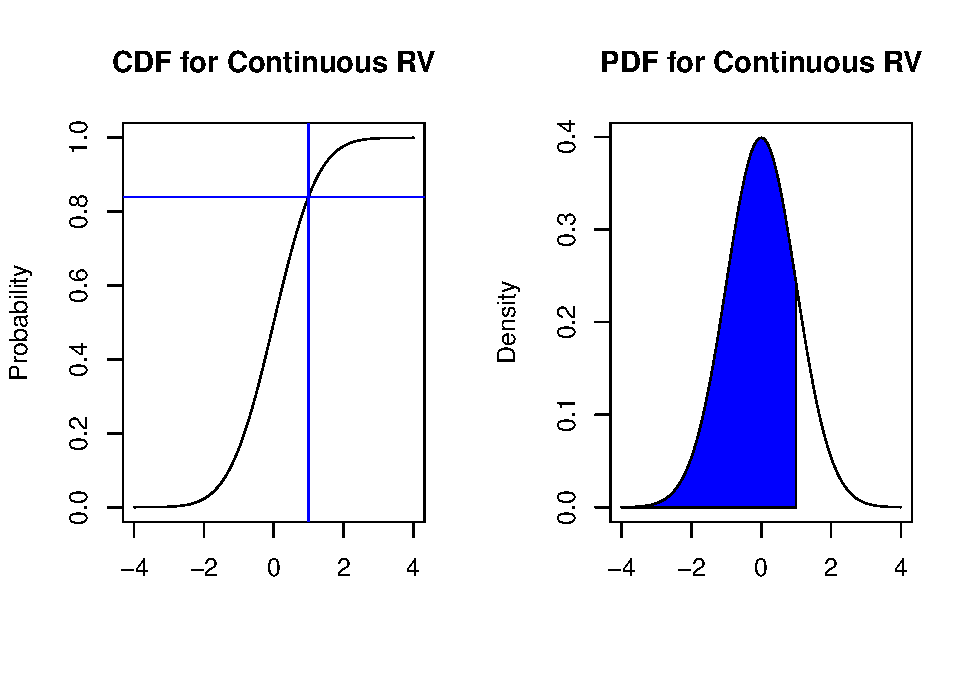
\includegraphics{bookdown-demo_files/figure-latex/4-prob-1.pdf}
\caption{\label{fig:4-prob}Probabilities from CDF and PDF}
\end{figure}

We can find \(P(X \leq 1)\) in two different ways:

\begin{itemize}
\tightlist
\item
  from the CDF, find the value of 1 on the horizontal axis, and read off the corresponding value on the vertical axis (blue lines). This tells us that \(P(X \leq 1) = 0.84\).
\item
  from the PDF, find the area under the PDF where \(X \leq 1\). This area corresponds to the shaded region in blue, and will be equal to 0.84 if we performed the integration per equation \eqref{eq:4-PDFCDF}.
\end{itemize}

Compare equation \eqref{eq:4-PDFCDF} with equation \eqref{eq:3-CDF} and note the similarities and differences in the CDFs for continuous and discrete random variables. For discrete CDFs, we sum the PMF over all values less than or equal to \(x\), whereas for continuous CDFs, we integrate, or accumulate the area, under the PDF over all values less than or equal to \(x\). Some people view the integral as a continuous version of a summation.

From equation \eqref{eq:4-PDFCDF}, we can generalize a way to find the probability \(P(a<X<b)\) for a continuous random variable \(X\):

\begin{equation} 
P(a<X<b) = F_X(b) - F_X(a) = \int_{a}^{b} f_X(x) dx.
\label{eq:4-integrate}
\end{equation}

In other words, to find the probability for a range of values for \(X\), we just find the area under its PDF for that range of values. Going back to our example, if we want to find \(P(0<X<1)\), we will find the area under its PDF for \(0<X<1\), like in Figure \ref{fig:4-prob2} below:

\begin{figure}
\centering
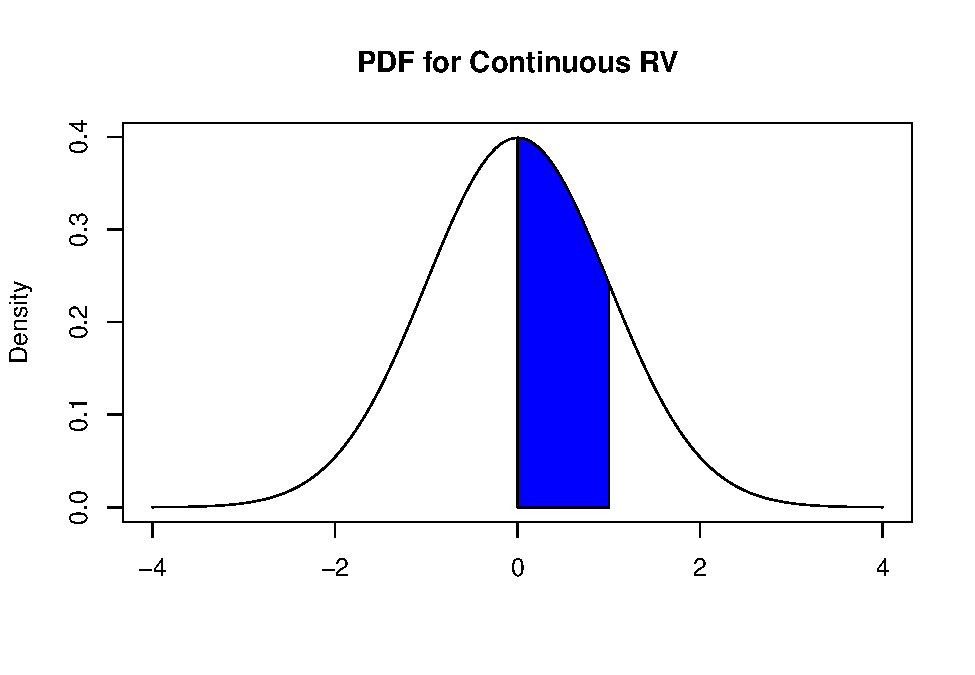
\includegraphics{bookdown-demo_files/figure-latex/4-prob2-1.pdf}
\caption{\label{fig:4-prob2}Probabilities from PDF}
\end{figure}

As mentioned, the PDF of a continuous random variable is analogous, but not exactly the same as, to the PMF of a discrete random variable. One common misconception is that the PDF tells us a probability, for example, that the value of \(f_X(2) = P(X=2)\), if \(X\) is continuous. This is only correct if \(X\) is discrete. In fact, if we look at equation \eqref{eq:4-integrate} a little more closely, \(P(X=c) = 0\) if \(X\) is continuous and \(c\) is a constant, since the area under its PDF will be 0.

\subsection{Valid PDFs}\label{valid-pdfs}

The PDF of a continuous random variable must satisfy the following criteria:

\begin{itemize}
\tightlist
\item
  Non negative: \(f_X(x) \geq 0\),
\item
  Integrates to 1: \(\int_{-\infty}^{\infty}f_X(x) dx = 1\).
\end{itemize}

\subsection{PDFs and Density Plots}\label{pdfs-and-density-plots}

Recall in Section \ref{pmfhist}, we learned that for discrete random variables, the PMF and histogram are related. The PMF represents the long-run proportion, while the histogram represents the relative frequency based on our data. As the sample size gets larger, the PMF should match the histogram.

Similarly for continuous random variables, the PDF and the density plot are related. The PDF is associated with the distribution of a known random variable, while the density plot is estimated from our data, and if our data follows a known random variable, the PDF should match the density plot as the sample size gets larger.

We will go over some of the details on how density plots are created at the end of this module, in Section \ref{KDE}, as we still need to cover a few concepts.

\section{Summaries of a Distribution}\label{summaries-of-a-distribution}

Next, we will talk about some common summaries associated with a distribution. These involve measures of centrality and variance, which we have covered before. We will also talk about a couple of other measures: skewness and kurtosis.

\subsection{Expectations}\label{expectations-1}

The \textbf{expected value} of a continuous random variable \(X\) is

\begin{equation} 
E(X) = \int_{-\infty}^{\infty} x f_X(x) dx.
\label{eq:4-EX}
\end{equation}

Another common notation for \(E(X)\) is \(\mu\), or sometimes \(\mu_X\) show that we are writing the mean of the random variable \(X\).

If we compare equation \eqref{eq:4-EX} with equation \eqref{eq:3-EX}, notice that we use an integral instead of a summation now that we are working with continuous random variables.

The interpretation of expected values is still the same: the expectation of a random variable can be interpreted as the long-run mean of the random variable, i.e.~if we were able to repeat the experiment an infinite number of times, the expectation of the random variable will be the average result among all the experiments. It is still a measure of centrality of the random variable.

The \textbf{linearity of expectations} still hold in the same way, per equation \eqref{eq:3-linEX}. It does not matter if the random variable is discrete or continuous.

The \textbf{Law of the Unconscious Statistician (LOTUS)} also still applies. For a continuous random variable \(X\), it is (unsurprisingly):

\begin{equation} 
E(g(X)) = \int_{-\infty}^{\infty} g(x) f_X(x).
\label{eq:4-lotus}
\end{equation}

Notice again when we compare equation \eqref{eq:4-lotus} with its discrete counterpart in equation \eqref{eq:3-lotus}: we have just replaced the summation with an integral.

\emph{Thought question}: Can you guess how to write the equation for the variance of a continuous random variable? Hint: the variance for a discrete random variable is given in equation \eqref{eq:3-var2}.

\subsubsection{Median}\label{median-1}

The value \(m\) is the \textbf{median} of a random variable \(X\) if \(P(X \leq c) \geq \frac{1}{2}\) and \(P(X \geq c) \geq \frac{1}{2}\).

Intuitively, the median is the value \(m\) which splits the area under the PDF into half (or as close to half as possible if the random variable is discrete). Half the area will be to the left of \(m\), the other half of the area will be to the right of \(m\).

\subsubsection{Mode}\label{mode-1}

For a continuous random variable \(X\), the \textbf{mode} is the value \(c\) that maximizes the PDF: \(f_X(c) \geq f_X(x)\) for all \(x\).

For a discrete random variable \(X\), the mode is the value \(c\) that maximizes the PMF: \(P(X=c) \geq P(X=x)\) for all \(x\). Intuitively, the mode is the most commonly occurring value of a discrete random variable

\subsubsection{Loss Functions}\label{loss-functions}

A goal of statistical modeling is to use a model to make predictions. We want to be able to quantify the quality of our prediction, or the prediction error. Suppose we have an experiment that can be described by a random variable \(X\), and we want to predict the value of the next experiment. The mean and median are natural guesses for the value of the next experiment.

It turns out there a several ways to quantify our prediction error. These are usually called \textbf{loss functions}. Suppose our predicted value is denoted by \(x_{pred}\). A couple of common loss functions are:

\begin{itemize}
\tightlist
\item
  \textbf{Mean squared error (MSE)}: \(E(X-x_{pred})^2\),
\item
  \textbf{Mean absolute error (MAE)}: \(E|X-x_{pred}|\).
\end{itemize}

It turns out that the expected value \(E(X)\) minimizes the MSE, and the median minimizes the MAE. So depending on what loss function suits our analysis, we could use either the mean or median for our predictions. We will cover these ideas in more detail in a later module (and indeed in later courses in this program).

\subsection{Variance}\label{variance-1}

The \textbf{variance} of a continuous random variable \(X\) is

\begin{equation} 
Var(X) = \int_{-\infty}^{\infty} (x-\mu)^2 f_X(x) dx.
\label{eq:4-var}
\end{equation}

The properties of variance is still the same as in Section \ref{var-prop}. It does not matter if the random variable is discrete or continuous. A common notation used for variance is \(\sigma^2\), or sometimes \(\sigma_X^2\) to show it is the variance of the random variable \(X\).

\subsection{Moments}\label{moments}

Before talking about other measures that are used to describe continuous distributions, we will cover some terminology that is used for these measures. Suppose we have a random variable \(X\).

\begin{itemize}
\tightlist
\item
  The \textbf{\(n\)th moment} of \(X\) is \(E(X^n)\). So the expected value, or the mean, is sometimes called the first moment.
\item
  The \textbf{\(n\)th central moment} of \(X\) is \(E((X-\mu)^n)\). So the variance is sometimes called the second central moment.
\item
  The \textbf{\(n\) standardized moment} of \(X\) is \(E(\frac{(X-\mu)^n}{\sigma})\).
\end{itemize}

\subsection{Skewness}\label{skewness}

One measure that is used to describe the shape of a distribution is skewness, which is a measure of symmetry (or measure of skewness). The \textbf{skew} of a random variable \(X\) is the third standardized moment:

\begin{equation} 
Skew(X) = E \left(\frac{(X-\mu)^3}{\sigma} \right)
\label{eq:4-skew}
\end{equation}

A random variable \(X\) has a \textbf{symmetric distribution about its mean} if \(X - \mu\) has the same distribution as \(\mu - X\). Fairly often, people will just say that \(X\) is symmetric; it is almost always assumed that the symmetry is about its mean.

Intuitively, symmetry means that the PDF of \(X\) to the left of its mean is the mirror image of the PDF of \(X\) to the right of its mean. We look at a couple of examples below in Figure \ref{fig:4-symm}:

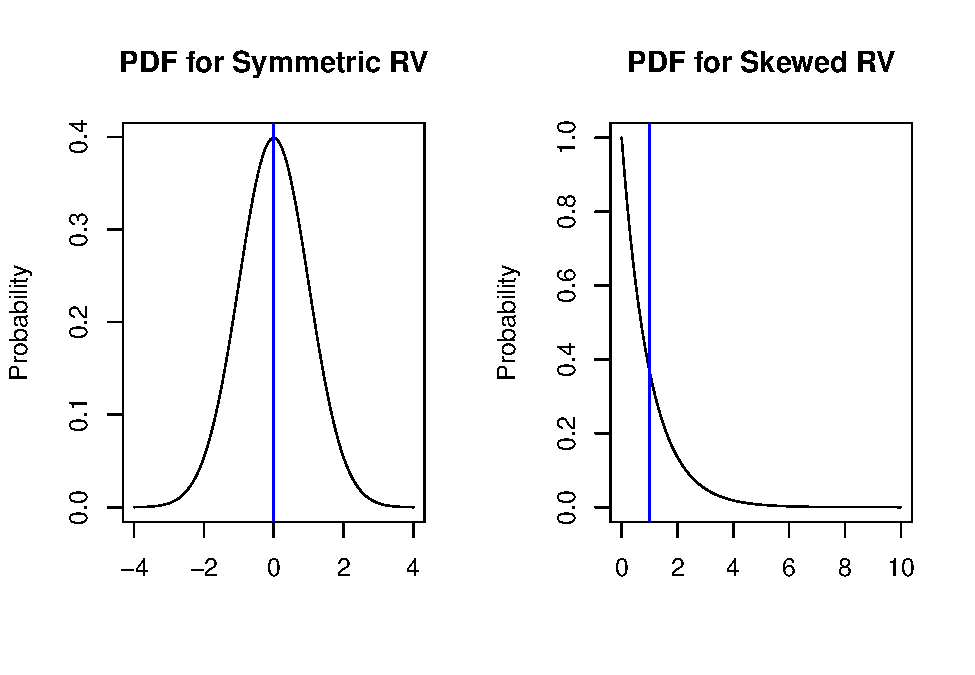
\includegraphics{bookdown-demo_files/figure-latex/4-symm-1.pdf}
The blue vertical lines indicate the mean of these distributions. Notice the mirror image in the first plot, but not in the second plot.

If a distribution is not symmetric, we can say its distribution is asymmetric, or is skewed. The values of \(Skew(X)\) that are associated with different shapes are:

\begin{itemize}
\tightlist
\item
  \(Skew(X) = 0\): \(X\) is symmetric.
\item
  \(Skew(X) > 0\): \(X\) is right (or positively) skewed.
\item
  \(Skew(X) < 0\): \(X\) is left (or negatively) skewed.
\end{itemize}

\subsection{Kurtosis}\label{kurtosis}

One more measure deals with the \textbf{tail} behavior of a distribution. Visually, the tails of a PDF are associated with probabilities of extreme values for a random variable. A distribution that is heavy tailed means that extreme values (on both ends) are more likely to occur. Tail behavior is an important consideration in risk management in finance: e.g.~a heavy left tail in the PDF could mean a financial crisis. Figure \ref{fig:4-kurt} shows an example of a heavy tailed distribution (in blue), compared to a Gaussian distribution (in black). We will talk more about the Gaussian distribution in the next subsection.

\begin{figure}
\centering
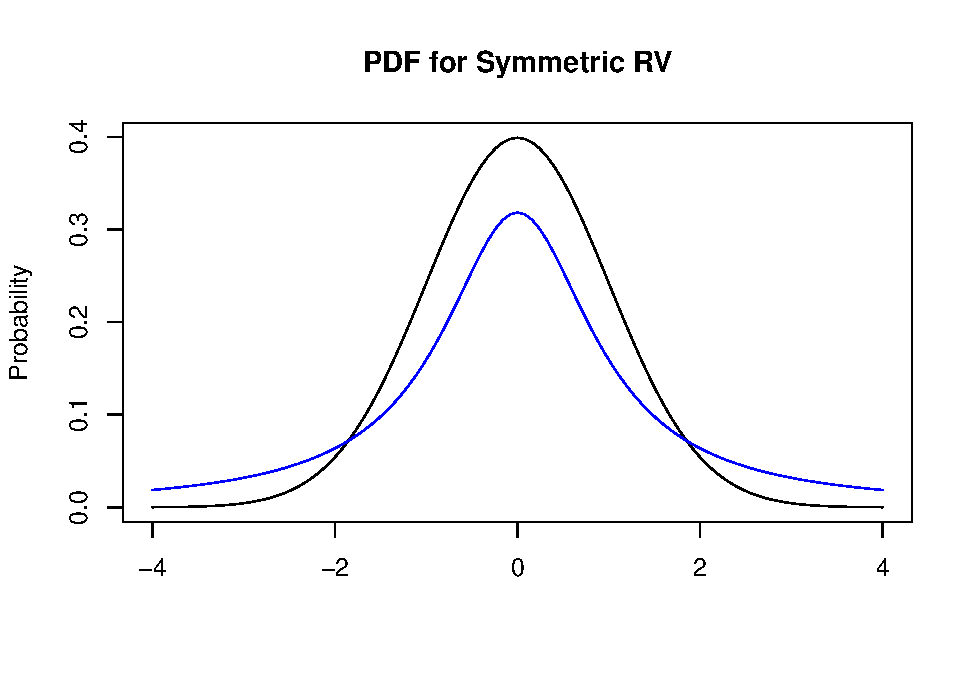
\includegraphics{bookdown-demo_files/figure-latex/4-kurt-1.pdf}
\caption{\label{fig:4-kurt}PDF for Heavy Tailed Distribution}
\end{figure}

A common measure of tail behavior is the \textbf{Kurtosis}. The kurtosis of a random variable \(X\) is the shifted fourth standardized moment:

\begin{equation} 
Kurt(X) = E \left(\frac{(X-\mu)^4}{\sigma} \right) - 3.
\label{eq:4-kurt}
\end{equation}

The reason for subtracting (or shifting by) 3 is so that the Gaussian distribution (a commonly used distribution for continuous random variables) has a kurtosis of 0. Note: Some authors call equation \eqref{eq:4-kurt} the \textbf{excess kurtosis} and the kurtosis does not subtract the 3.

The values of \(Kurt(X)\) that are associated with tail behaviors are:

\begin{itemize}
\tightlist
\item
  \(Kurt(X) = 0\): \(X\) is similar tails to Gaussian distribution.
\item
  \(Kurt(X) > 0\): \(X\) has heavier tails compared to Gaussian distribution (extreme values more likely).
\item
  \(Kurt(X) < 0\): \(X\) has smaller tails compared to Gaussian distribution (extreme values less likely).
\end{itemize}

\section{Common Continuous Random Variables}\label{common-continuous-random-variables}

Next, we will introduce some commonly used distributions that may be used for continuous random variables. A number of common statistical models (for example, linear regression) are based on these distributions.

\subsection{Uniform}\label{uniform}

A random variable that follows a uniform distribution on the interval \((a,b)\) is a completely random number between \(a\) and \(b\). Notionally, an upper case \(U\) is usually used to denote a uniform random variable. \(U\) is said to have a \textbf{uniform distribution} on the interval \((a,b)\), denoted as \(U \sim(a,b)\), if its PDF is

\begin{equation} 
f_X(x) = \begin{cases} 
  \frac{1}{b-a} & \text{if } a<x<b \\
  0 & \text{otherwise }. 
\end{cases}
\label{eq:4-U}
\end{equation}

Note that the parameters \(a,b\) also help define the support of a uniform distribution. Figure \ref{fig:4-U} below displays a plot of the PDF of a \(U(a,b)\):

\begin{figure}
\centering
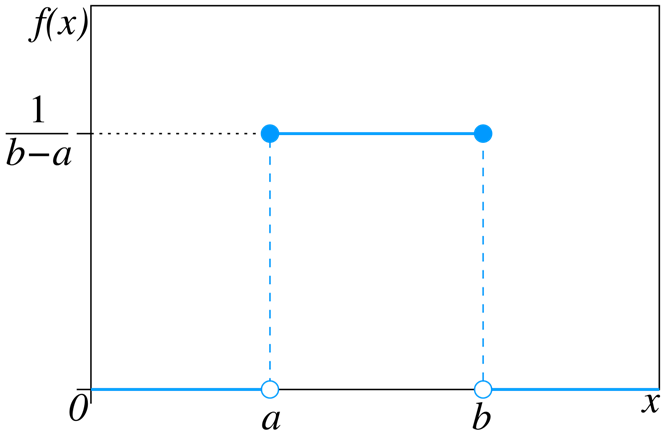
\includegraphics{images/04-U.png}
\caption{\label{fig:4-U}PDF of U(a,b). Picture from \url{https://en.wikipedia.org/wiki/Continuous_uniform_distribution}}
\end{figure}

\emph{Thought question}: Can you verify that this is a valid PDF?

Figure \ref{fig:4-Ucdf} below displays a plot of the CDF of a \(U(a,b)\):

\begin{figure}
\centering
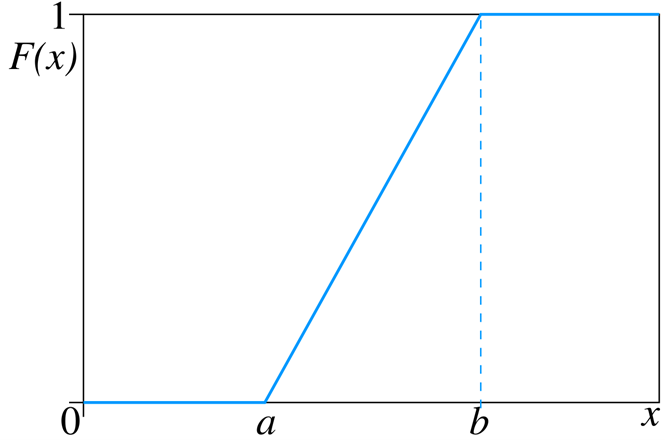
\includegraphics{images/04-Ucdf.png}
\caption{\label{fig:4-Ucdf}CDF of U(a,b). Picture from \url{https://en.wikipedia.org/wiki/Continuous_uniform_distribution}}
\end{figure}

Some properties of the uniform distribution:

\begin{itemize}
\tightlist
\item
  Its mean is \(E(U) = \frac{a+b}{2}\).
\item
  Its variance is \(Var(U) = \frac{(b-a)^2}{12}\).
\item
  Its skewness is 0, so it is symmetric.
\item
  Its kurtosis is -\(\frac{6}{5}\), so its tails are not as heavy compared to a Gaussian distribution.
\end{itemize}

\emph{Thought question}: Can you see why a uniform distribution is symmetric? Can you see why its tails are not heavy?

If the support of a uniform distribution is between 0 and 1, we have a \textbf{standard uniform distribution}. We will talk about the importance of the standard uniform distribution in the next subsection.

\subsubsection{Universality of Uniform}\label{universality-of-uniform}

It turns out that we can construct a random variable with any continuous distribution based on a standard uniform distribution. This fact is used to simulate random numbers from continuous distributions. This fact is called the \textbf{Universality of the Uniform}: Let \(F_X(x)\) denote the CDF of a continuous random variable \(X\), then:

\begin{enumerate}
\def\labelenumi{\arabic{enumi}.}
\tightlist
\item
  Let \(U \sim U(0,1)\) and \(X = F^{-1}(U)\). Then \(X\) is a random variable with CDF \(F_X(x)\).
\item
  \(F_X(X) \sim U(0,1)\).
\end{enumerate}

To give some insight into what this means, we look at an example. Another continuous distribution is called the standard logistic distribution, which we will denote with \(X\). Its CDF is

\[
F_X(x) = \frac{e^x}{1+e^x}.
\]
Let \(U \sim U(0,1)\). The first part of the universality of the uniform informs us that the inverse of the CDF for the standard logistic is \(F_X^{-1}(U) \sim X\), so we invert \(F_X(x)\) to get its inverse \(F_X^{-1}(x)\). This is done by setting the CDF of \(X\) to be equal to \(u\), i.e.~let \(u = \frac{e^x}{1+e^x}\), and solving for \(x\):

\[
\begin{split}
u + u e^x &= e^x\\
\implies u &= e^x (1-u) \\
\implies e^x &= \frac{u}{1-u} \\
\implies x &= \log (\frac{u}{1-u}).
\end{split}
\]

Therefore \(F^{-1}(u) = \log (\frac{u}{1-u})\) and \(F^{-1}(U) = \log (\frac{U}{1-U})\). Therefore \(\log (\frac{U}{1-U})\) follows a standard logistic distribution.

Let us use simulations to show what is going on. First, we simulate 10,000 reps from a standard uniform distribution, then invert these values using \(\log (\frac{u}{1-u})\), and create the density plot of \(\log (\frac{u}{1-u})\). These steps are shown in Figure \ref{fig:4-universe} below:

\begin{Shaded}
\begin{Highlighting}[]
\FunctionTok{set.seed}\NormalTok{(}\DecValTok{4}\NormalTok{)}

\NormalTok{reps}\OtherTok{\textless{}{-}}\DecValTok{10000} \DocumentationTok{\#\#number of reps}
\NormalTok{u}\OtherTok{\textless{}{-}}\FunctionTok{runif}\NormalTok{(reps) }\DocumentationTok{\#\#simulate standard uniform}
\NormalTok{invert}\OtherTok{\textless{}{-}} \FunctionTok{log}\NormalTok{(u}\SpecialCharTok{/}\NormalTok{(}\DecValTok{1}\SpecialCharTok{{-}}\NormalTok{u)) }\DocumentationTok{\#\#invert based on F inverse. These should now follow standard logistic}

\FunctionTok{par}\NormalTok{(}\AttributeTok{mfrow=}\FunctionTok{c}\NormalTok{(}\DecValTok{1}\NormalTok{,}\DecValTok{3}\NormalTok{))}
\FunctionTok{plot}\NormalTok{(}\FunctionTok{density}\NormalTok{(u), }\AttributeTok{main=}\StringTok{"Density Plot from 10,000 U\textquotesingle{}s"}\NormalTok{)}
\FunctionTok{plot}\NormalTok{(}\FunctionTok{density}\NormalTok{(invert), }\AttributeTok{main=}\StringTok{"Density Plot after Inverting"}\NormalTok{, }\AttributeTok{xlim=}\FunctionTok{c}\NormalTok{(}\SpecialCharTok{{-}}\DecValTok{6}\NormalTok{,}\DecValTok{6}\NormalTok{))}
\FunctionTok{curve}\NormalTok{(dlogis, }\AttributeTok{from =} \SpecialCharTok{{-}}\DecValTok{7}\NormalTok{, }\AttributeTok{to =} \DecValTok{7}\NormalTok{, }\AttributeTok{main =} \StringTok{"PDF for Logistic"}\NormalTok{, }\AttributeTok{ylab=}\StringTok{"Density"}\NormalTok{, }\AttributeTok{xlab=}\StringTok{""}\NormalTok{)}
\end{Highlighting}
\end{Shaded}

\begin{figure}
\centering
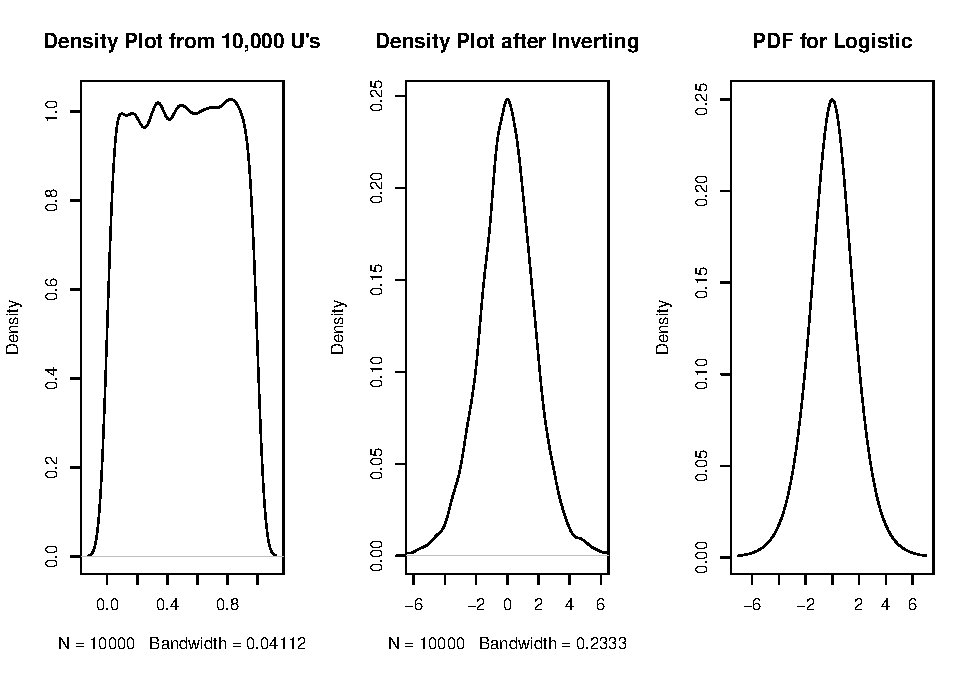
\includegraphics{bookdown-demo_files/figure-latex/4-universe-1.pdf}
\caption{\label{fig:4-universe}Uniform to Logistic}
\end{figure}

From Figure \ref{fig:4-universe}:

\begin{itemize}
\tightlist
\item
  The first plot shows the density plot from our 10,000 reps from a standard normal. This is close to the PDF of a standard uniform.
\item
  The second plot shows the density plot after inverting our 10,000 reps from a standard normal, i.e.~\(F^{-1}(u) = \log (\frac{u}{1-u})\).
\item
  The third plot shows the PDF of a standard logistic. Notice how similar this looks to the second plot.
\end{itemize}

So we see that \(\log (\frac{U}{1-U})\) follows a standard logistic distribution.

The second part of the universality of the uniform informs us that if \(X\) follows a standard logistic distribution, then \(F(X) = \frac{e^X}{1 + e^X} \sim U(0,1)\).

So, we can see the purpose of the universality of the uniform:

\begin{itemize}
\tightlist
\item
  For part 1, we can simulate reps from any distribution, as long as we know its CDF. The software you use may not be able to simulate reps from a particular distribution, but you can write code to simulate reps from this distribution based on the standard uniform.
\item
  For part 2, we can convert a random variable with an unknown distribution to one that is known: the standard uniform.
\end{itemize}

\subsection{Normal}\label{normdist}

Another widely used distribution for continuous random variables is the \textbf{normal}, or \textbf{Gaussian} distribution. This is a distribution that is symmetric and bell-shaped. This is probably the most important distribution in statistics and data science due to the Central Limit Theorem. We will define this theorem in a later module, but loosely speaking, it says that if we take the average of a bunch of random variables, the average will approximate a normal distribution, even if the random variables are individually not normal.

A lot of questions that we wish to answer are based on averages. For example

\begin{itemize}
\tightlist
\item
  Does the implementation of certain technologies in a class improve test scores for students, on average?
\item
  Are male Gentoo penguins heavier than their female counterparts, on average?
\item
  Does replacing traffic lights with a roundabout reduce the number of traffic accidents, on average?
\end{itemize}

What the central limit theorem implies is that even if test scores, weights of Gentoo penguins, and number of traffic accidents do not follow a normal distribution, their average values will approximate a normal distribution.

\subsubsection{Standard Normal}\label{standard-normal}

First, we will talk about the \textbf{standard normal distribution}, as other normal distributions can be viewed as variations of the standard normal. A standard normal distribution has mean 0 and variance 1. It is usually denoted by \(Z\). We can also write \(Z \sim N(0,1)\) to say that \(Z\) is normally distributed with mean 0 and variance 1. The PDF of a standard normal distribution is:

\begin{equation} 
\phi(z) = \frac{1}{\sqrt{2 \pi}} e^{-z^2/2}.
\label{eq:4-Z}
\end{equation}

Notice the constant \(\frac{1}{\sqrt{2 \pi}}\) in equation \eqref{eq:4-Z}. Its presence is needed to make the PDF valid, since the PDF must integrate to 1. Such constants are called \textbf{normalizing constants}.

Figure \ref{fig:4-Z} below displays its PDF:

\begin{Shaded}
\begin{Highlighting}[]
\FunctionTok{curve}\NormalTok{(dnorm, }\AttributeTok{from =} \SpecialCharTok{{-}}\DecValTok{4}\NormalTok{, }\AttributeTok{to =} \DecValTok{4}\NormalTok{, }\AttributeTok{main =} \StringTok{"PDF for Z"}\NormalTok{, }\AttributeTok{ylab=}\StringTok{"Density"}\NormalTok{, }\AttributeTok{xlab=}\StringTok{""}\NormalTok{)}
\end{Highlighting}
\end{Shaded}

\begin{figure}
\centering
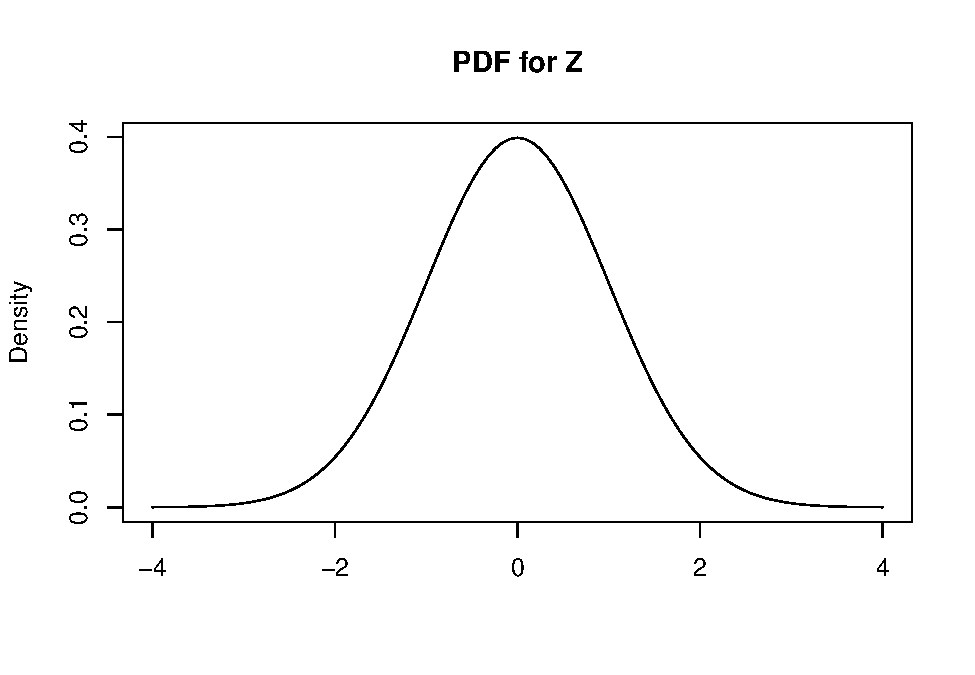
\includegraphics{bookdown-demo_files/figure-latex/4-Z-1.pdf}
\caption{\label{fig:4-Z}PDF of Standard Normal}
\end{figure}

From Figure \ref{fig:4-Z}, we can see the following properties of a standard normal distribution (these will apply for any normal distribution):

\begin{itemize}
\tightlist
\item
  Its PDF is symmetric about its mean. In Figure \ref{fig:4-Z}, the PDF is symmetric about 0, i.e.~\(\phi(-z) = \phi(z)\).
\item
  This implies that the tail areas are also symmetric. For example, \(P(Z \leq -2) = P(Z \geq 2)\).
\item
  Its skew is 0, since it is symmetric.
\end{itemize}

There is actually no closed-formed equation for the CDF of a standard normal (or any normal distribution). We write \(\Phi(z) = P(Z \leq z) = \int_{\infty}^z \phi(z) dz\) to express the CDF of a standard normal.

Notice that we have special letters \(Z, \phi, \Phi\) to denote the standard normal distribution. This is an indication of how often it is used to warrant its own notation.

\subsubsection{From Standard Normal to Other Normals}\label{norm}

If \(Z \sim N(0,1)\), then \(X = \mu + \sigma Z \sim N(\mu, \sigma^2)\). In other words, if \(Z\) is standard normal, then \(X = \mu + \sigma Z\) follows a normal distribution with mean \(\mu\) and variance \(\sigma^2\). The parameters of a normal distribution are the mean \(\mu\) and variance \(\sigma^2\).

Note that some authors say the parameters are the mean \(\mu\) and standard deviation \(\sigma\) instead, so be careful when reading notation associated with normal distributions from various sources. For example, \(N(0,2)\) in our class and our book means normal distribution with mean 0 and variance 2, but for some other authors, \(N(0,2)\) means normal distribution with mean 0 and standard deviation 2. Indeed, the functions in R use this alternate parameterization, so you need to be careful.

\emph{Thought question}: Can you use the linearity of expectations to explain why \(X\) has mean \(\mu\)? Can you use properties of variance from Section \ref{var-prop} to explain why \(X\) has variance \(\sigma^2\)?

Notice how we started from a standard normal \(Z\), and transformed \(Z\) by multiplying it by \(\sigma\) and then adding \(\mu\) to get any normal distribution. This transformation is called a \textbf{location-scale} transformation, or shifting and scaling. The scale changes since we multiply by a constant \(\sigma\); the location is transformed since its mean changes from 0 to \(\mu\).

We can also reverse this transformation and state the following: If \(X \sim N(\mu, \sigma^2)\), then \(Z = \frac{X-\mu}{\sigma} \sim N(0,1)\). If we start with \(X \sim N(\mu, \sigma^2)\), then we can transform \(X\) by subtracting \mu, and then dividing by \(\sigma\), to obtain \(Z\). This particular transformation is called \textbf{standardization}:

\begin{equation} 
Z = \frac{X-\mu}{\sigma}.
\label{eq:4-standardize}
\end{equation}

The PDF of any normal distribution \(X \sim N(\mu, \sigma^2)\) is

\begin{equation} 
f_X(x) = \frac{1}{\sigma \sqrt{2 \pi}} \exp \left(-\frac{(x - \mu)^2}{2 \sigma^2} \right).
\label{eq:4-pdfNormal}
\end{equation}

\emph{Thought question}: Compare equations \eqref{eq:4-pdfNormal} and \eqref{eq:4-Z}. Can you see how equation \eqref{eq:4-Z} can be derived from equation \eqref{eq:4-pdfNormal}?

\subsubsection{68-95-99.7\% Rule}\label{rulenorm}

The following property holds for any normal distribution, and is often called the \textbf{68-99-99.7\%} rule. For any normal distribution \(X \sim N(\mu, \sigma^2)\):

\begin{itemize}
\tightlist
\item
  \(P(\mu - \sigma < X < \mu + \sigma) \approx 0.68\),
\item
  \(P(\mu - 2\sigma < X < \mu + 2\sigma) \approx 0.95\),
\item
  \(P(\mu - 3\sigma < X < \mu + 3\sigma) \approx 0.997\).
\end{itemize}

What these mean is that for any normal distribution:

\begin{itemize}
\tightlist
\item
  About 68\% of observed values will fall within 1 standard deviation of the mean,
\item
  About 95\% of observed values will fall within 2 standard deviations of the mean, and
\item
  About 99.7\% of observed values will fall within 3 standard deviations of the mean.
\end{itemize}

The last statement is the basis for the term \href{https://en.wikipedia.org/wiki/Six_Sigma}{six sigma} used in manufacturing, since virtually all data points should fall within a range that is six sigma wide (assuming they follow a normal distribution). Visually, this rule is shown in Figure \ref{fig:4-rule} when applied to the standard normal:

\begin{figure}
\centering
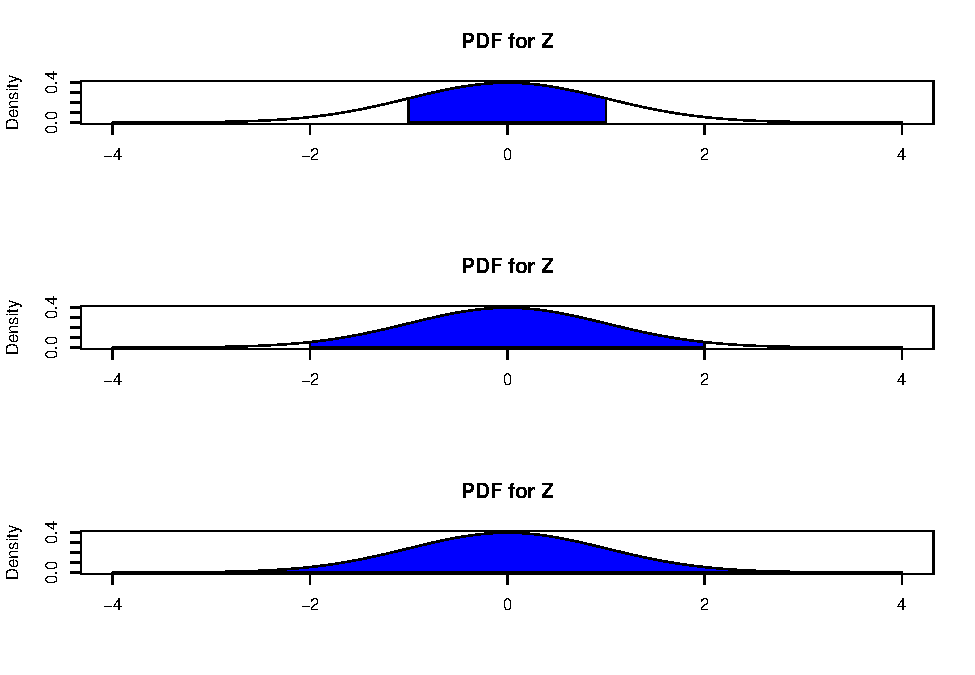
\includegraphics{bookdown-demo_files/figure-latex/4-rule-1.pdf}
\caption{\label{fig:4-rule}68-95-99.7 Rule}
\end{figure}

We will work out the first statement, that about 68\% of the observed values will fall within 1 standard deviation of the mean for any normal distribution. We will use R to help us verify this rule for a standard normal:

\begin{Shaded}
\begin{Highlighting}[]
\NormalTok{upper1}\OtherTok{\textless{}{-}}\FunctionTok{pnorm}\NormalTok{(}\DecValTok{1}\NormalTok{) }\DocumentationTok{\#\# what is percentile associated with Z=1 (i.e. 1 standard deviation above mean)}
\NormalTok{lower1}\OtherTok{\textless{}{-}}\FunctionTok{pnorm}\NormalTok{(}\SpecialCharTok{{-}}\DecValTok{1}\NormalTok{) }\DocumentationTok{\#\# what is percentile associated with Z={-}1 (i.e. 1 standard deviation below mean)}
\NormalTok{upper1}\SpecialCharTok{{-}}\NormalTok{lower1 }\DocumentationTok{\#\# find proportion in between 1 SD above and below mean.}
\end{Highlighting}
\end{Shaded}

\begin{verbatim}
## [1] 0.6826895
\end{verbatim}

\emph{Thought question}: how would you tweak this code to verify the other two statements associated with the 68-95-99.7\% rule?

\section{Using R}\label{using-r}

R has built in functions to compute the density, CDF, percentiles, as well as simulate data of common distributions. We will start with a random variable \(Y \sim N(1, 9)\) as an example.

\begin{enumerate}
\def\labelenumi{\arabic{enumi}.}
\tightlist
\item
  To find \(f_Y(2)\), use:
\end{enumerate}

\begin{Shaded}
\begin{Highlighting}[]
\FunctionTok{dnorm}\NormalTok{(}\DecValTok{2}\NormalTok{, }\DecValTok{1}\NormalTok{, }\DecValTok{3}\NormalTok{) }\DocumentationTok{\#\#supply the value of Y you want, then the parameters mu and sigma}
\end{Highlighting}
\end{Shaded}

\begin{verbatim}
## [1] 0.1257944
\end{verbatim}

The density \(f_Y(2)\) is 0.1257944. Note: In R, the normal distribution is parameterized by the mean and standard deviation, which is different from these set of notes and our book, which uses the mean and variance.

\begin{enumerate}
\def\labelenumi{\arabic{enumi}.}
\setcounter{enumi}{1}
\tightlist
\item
  To find \(P(Y \leq 2)\), use:
\end{enumerate}

\begin{Shaded}
\begin{Highlighting}[]
\FunctionTok{pnorm}\NormalTok{(}\DecValTok{2}\NormalTok{, }\DecValTok{1}\NormalTok{, }\DecValTok{3}\NormalTok{) }\DocumentationTok{\#\#supply the value of Y you want, then the parameters mu and sigma}
\end{Highlighting}
\end{Shaded}

\begin{verbatim}
## [1] 0.6305587
\end{verbatim}

The probability that \(Y\) is less than or equal to 2 is 0.6305587.

Alternatively, we can standardize this normal distribution, and use the standard normal. The standardization, per equation \eqref{eq:4-standardize}, gives us

\[
z = \frac{2-1}{3} = \frac{1}{3},
\]

so

\[
\begin{split}
P(Y \leq 2) &= P(\frac{Y-\mu}{\sigma} \leq \frac{2-1}{3}) \\
            &= P(Z \leq \frac{1}{3}) \\
            &= \Phi(\frac{1}{3})
\end{split}
\]

which can be found using

\begin{Shaded}
\begin{Highlighting}[]
\FunctionTok{pnorm}\NormalTok{(}\DecValTok{1}\SpecialCharTok{/}\DecValTok{3}\NormalTok{) }\DocumentationTok{\#\#don\textquotesingle{}t supply mu and sigma means you want to use standard normal}
\end{Highlighting}
\end{Shaded}

\begin{verbatim}
## [1] 0.6305587
\end{verbatim}

which gives the same answer as \texttt{pnorm(2,1,3)}.

\begin{enumerate}
\def\labelenumi{\arabic{enumi}.}
\setcounter{enumi}{2}
\tightlist
\item
  To find the value on the support that corresponds to the 90th percentile, use:
\end{enumerate}

\begin{Shaded}
\begin{Highlighting}[]
\FunctionTok{qnorm}\NormalTok{(}\FloatTok{0.9}\NormalTok{, }\DecValTok{1}\NormalTok{, }\DecValTok{3}\NormalTok{) }\DocumentationTok{\#\#supply the value of the percentile you need, then the parameters mu and sigma}
\end{Highlighting}
\end{Shaded}

\begin{verbatim}
## [1] 4.844655
\end{verbatim}

The 90th percentile of \(Y \sim N(1,9)\) is 4.844655.

If we want to use the standard normal, we could find its 90th percentile:

\begin{Shaded}
\begin{Highlighting}[]
\FunctionTok{qnorm}\NormalTok{(}\FloatTok{0.9}\NormalTok{)}
\end{Highlighting}
\end{Shaded}

\begin{verbatim}
## [1] 1.281552
\end{verbatim}

and then apply the location scale transformation

\begin{Shaded}
\begin{Highlighting}[]
\FunctionTok{qnorm}\NormalTok{(}\FloatTok{0.9}\NormalTok{)}\SpecialCharTok{*}\DecValTok{3} \SpecialCharTok{+} \DecValTok{1} \DocumentationTok{\#\#multiply by sigma, then add mu}
\end{Highlighting}
\end{Shaded}

\begin{verbatim}
## [1] 4.844655
\end{verbatim}

which is the same answer as \texttt{qnorm(0.9,1,3)}.

\begin{enumerate}
\def\labelenumi{\arabic{enumi}.}
\setcounter{enumi}{3}
\tightlist
\item
  To simulate 10 draws (replicates) of \(Y\), use:
\end{enumerate}

\begin{Shaded}
\begin{Highlighting}[]
\FunctionTok{set.seed}\NormalTok{(}\DecValTok{2}\NormalTok{) }\DocumentationTok{\#\#use set.seed() so we get the same random numbers each time the code is run}
\FunctionTok{rnorm}\NormalTok{(}\DecValTok{10}\NormalTok{, }\DecValTok{1}\NormalTok{, }\DecValTok{3}\NormalTok{) }\DocumentationTok{\#\#supply the number of simulated data you need, then the parameters mu and sigma}
\end{Highlighting}
\end{Shaded}

\begin{verbatim}
##  [1] -1.6907436  1.5545476  5.7635360 -2.3911270  0.7592447  1.3972609
##  [7]  3.1238642  0.2809059  6.9534218  0.5836390
\end{verbatim}

This outputs a vector of length 10. Each value represents the result of each rep. So the first value drawn from \(Y \sim N(1,9)\) -1.6907436, the second value drawn is 1.5545476 and so on.

Just like in Section \ref{Rdis}, notice these functions all ended with \texttt{norm}. We just added a different letter first, depending on whether we want the density (analogous to PDF), CDF, percentile, or random draw. The letters are \texttt{d}, \texttt{p}, \texttt{q}, and \texttt{r} respectively.

One thing to note: if we do not supply the mean and standard deviation, for example we type \texttt{rnorm(10)}, R will assume you want to use a standard normal distribution, so \texttt{rnorm(10)} will draw 10 random numbers from a standard normal.

\subsection{Density Plots and Kernel Density Estimation}\label{KDE}

We are now ready to talk about how density plots, like the ones in Figure \ref{fig:4-universe} are created. Recall the difference between density plots and PDFs:

\begin{itemize}
\tightlist
\item
  A plot of the PDF describes the distribution of a known random variable.
\item
  A density plot is based on our data, and is used to describe the distribution of our data. Our data may or may not follow a commonly known random variable. If it does, then a plot of the PDF and the density plot should match up as we gather more and more data.
\end{itemize}

Proportions are found in the same way, by finding the area under the PDF or density plot for the appropriate range on the support.

Suppose we have \(n\) observed values of an unknown random variable \(X\): \(x_1, x_2, \cdots, x_n\).The density \(f\) of \(X\) is unknown and we want to estimate it with our data. To estimate the density \(f\), we use the \textbf{kernel density estimator}:

\begin{equation} 
\hat{f}_h(x) = \frac{1}{nh} \sum_{i=1}^n K \left( \frac{x-x_i}{h}\right ),
\label{eq:4-KDE}
\end{equation}

where \(K\) is the \textbf{kernel} and \(h\) is a smoothing parameter, often called the \textbf{bandwidth}. Looking at equation \eqref{eq:4-KDE}, the KDE can be viewed as a weighted average of the relative likelihood of observing a particular value.

The kernel can be viewed as a weighting function, with the weights following the shape of a distribution that the user specifies (usually symmetric). Common kernel functions and their shapes are displayed in Figure \ref{fig:4-KDE}:

\begin{figure}
\centering
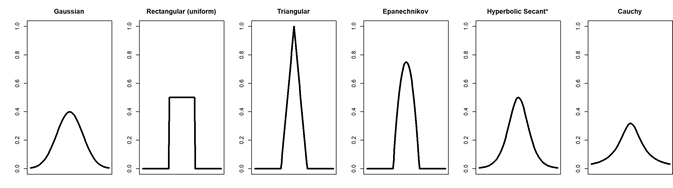
\includegraphics{images/04-KDE.png}
\caption{\label{fig:4-KDE}Common Kernals. Picture adapted from \url{https://tgstewart.cloud/compprob/kde.html}}
\end{figure}

The horizontal axis on the kernel can be viewed as the distance of the value of a data point from a specific value on the support, and the mid point on the horizontal axis represents a distance of 0.

\begin{itemize}
\tightlist
\item
  Looking at the normal kernel, nearest values receive the highest weight, and values further away receive less weight.
\item
  For the uniform kernel, values within a certain distance receive a weight, and values beyond a certain distance receive no weight.
\item
  The Epanechnikov (parabolic) kernel is a mix of both: values beyond a certain distance receive no weight, and values within a certain distance receive a weight that is roughly inversely proportional to the distance.
\end{itemize}

\(h\) is the smoothing parameter and is analogous to bin width in histograms. Larger values result in smoother looking density plots.

Let us go back to an old example. We will use the \texttt{loan50} dataset from the \texttt{openintro} package. The data originally consist of thousands of loans made through the Lending Club platform, but we will randomly select 50 of these loans. Let us study the interest rate the loans the 50 applicants received.

\begin{Shaded}
\begin{Highlighting}[]
\FunctionTok{library}\NormalTok{(openintro)}

\DocumentationTok{\#\#create object for data}
\NormalTok{Data}\OtherTok{\textless{}{-}}\NormalTok{loan50}

\DocumentationTok{\#\#create density plot using default}
\FunctionTok{plot}\NormalTok{(}\FunctionTok{density}\NormalTok{(Data}\SpecialCharTok{$}\NormalTok{interest\_rate), }\AttributeTok{main=}\StringTok{"Density Plot of Interest Rates"}\NormalTok{)}
\end{Highlighting}
\end{Shaded}

\begin{figure}
\centering
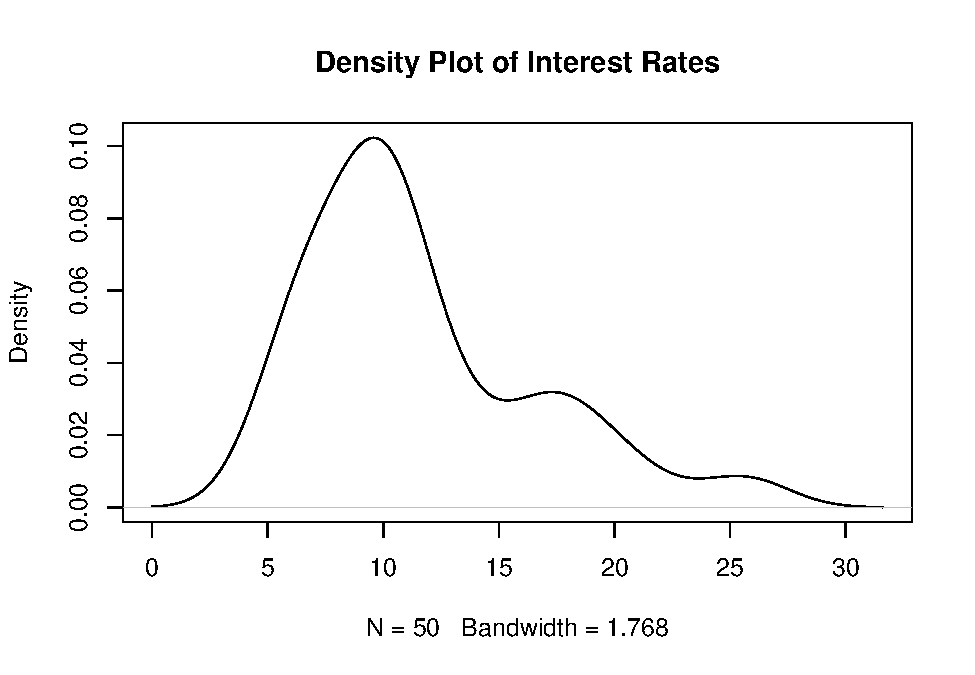
\includegraphics{bookdown-demo_files/figure-latex/4-R-1.pdf}
\caption{\label{fig:4-R}Density Plot for 50 Interest Rates}
\end{figure}

This uses KDE with the default settings: kernel is normal, and the bandwidth is based on \href{https://en.wikipedia.org/wiki/Kernel_density_estimation\#A_rule-of-thumb_bandwidth_estimator}{Silverman's rule of thumb}.

To change these, we add the \texttt{kernel} and \texttt{adjust} argument when using the \texttt{density()} function, for example, to use the Epanechnikov kernal with twice the default bandwidth:

\begin{Shaded}
\begin{Highlighting}[]
\DocumentationTok{\#\#create density plot using different settings}
\FunctionTok{plot}\NormalTok{(}\FunctionTok{density}\NormalTok{(Data}\SpecialCharTok{$}\NormalTok{interest\_rate, }\AttributeTok{kernel =} \StringTok{"epanechnikov"}\NormalTok{, }\AttributeTok{adjust =} \DecValTok{2}\NormalTok{), }
     \AttributeTok{main=}\StringTok{"Density Plot of Interest Rates"}\NormalTok{)}
\end{Highlighting}
\end{Shaded}

\begin{figure}
\centering
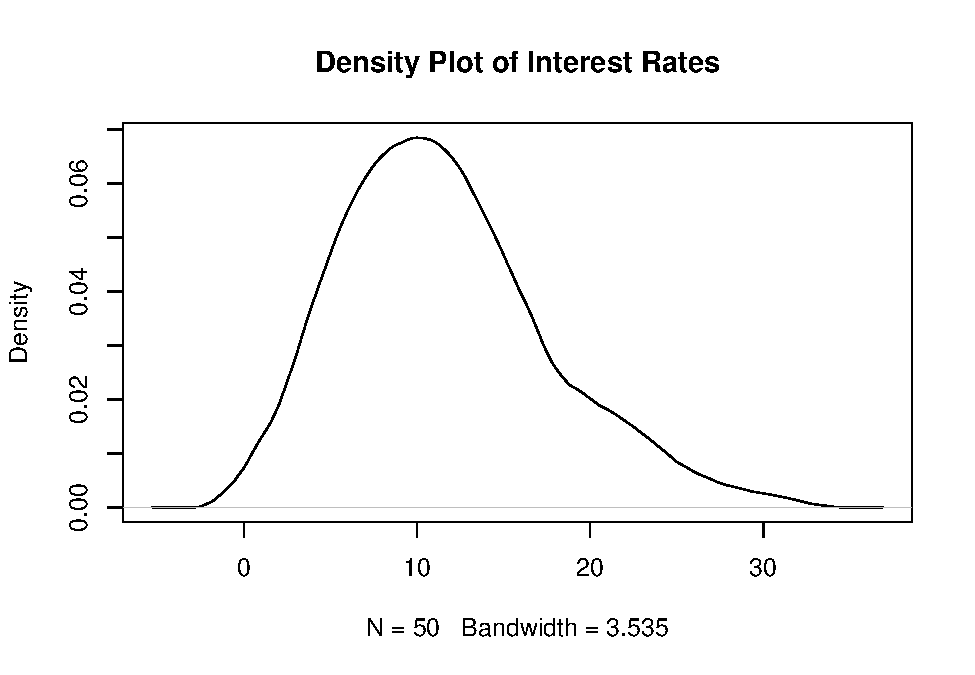
\includegraphics{bookdown-demo_files/figure-latex/4-R2-1.pdf}
\caption{\label{fig:4-R2}Density Plot for 50 Interest Rates, Epanechnikov Kernel, Twice the Bandwidth}
\end{figure}

The density plot in Figure \ref{fig:4-R2} looks smoother than the density plot in Figure \ref{fig:4-R}.

\subsection{Density Plots and Histograms}\label{density-plots-and-histograms}

In Section \ref{densplots}, we mentioned that density plots can be viewed as smoothed versions of a histogram. We create a histogram of interest rates, and overlay a density plot in blue, per Figure \ref{fig:4-R3} below:

\begin{Shaded}
\begin{Highlighting}[]
\FunctionTok{hist}\NormalTok{(Data}\SpecialCharTok{$}\NormalTok{interest\_rate, }\AttributeTok{prob =} \ConstantTok{TRUE}\NormalTok{, }\AttributeTok{main =} \StringTok{"Histogram with Density Plot"}\NormalTok{, }\AttributeTok{xlab=}\StringTok{"Interest Rates"}\NormalTok{)}

\DocumentationTok{\#\#create density plot using default}
\FunctionTok{lines}\NormalTok{(}\FunctionTok{density}\NormalTok{(Data}\SpecialCharTok{$}\NormalTok{interest\_rate), }\AttributeTok{col=}\StringTok{"blue"}\NormalTok{)}
\end{Highlighting}
\end{Shaded}

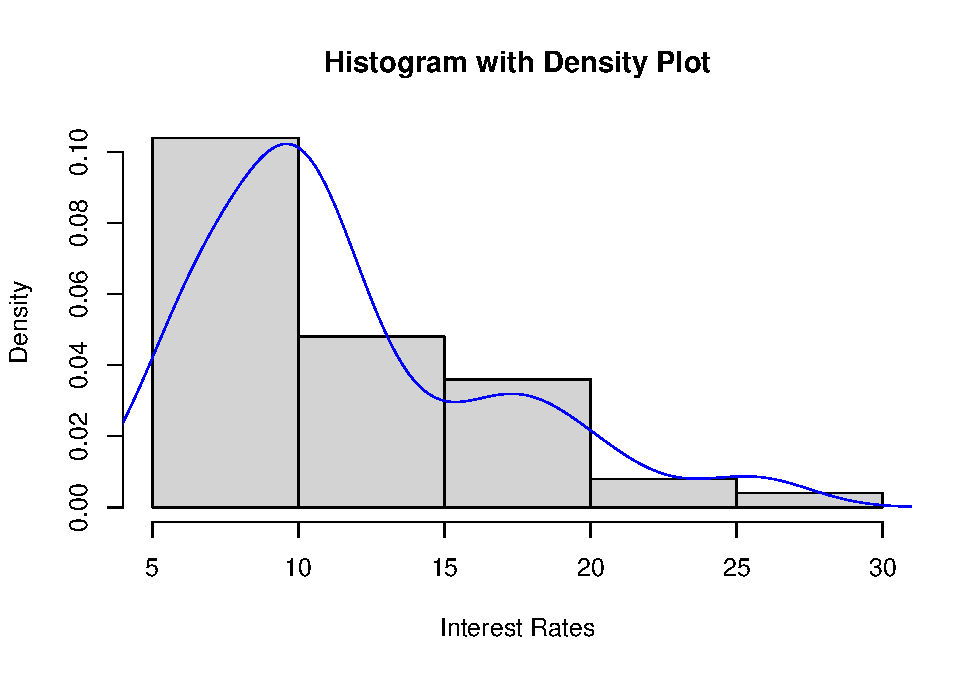
\includegraphics{bookdown-demo_files/figure-latex/4-R3-1.pdf}
Notice how the density plot approximates the histogram.

\subsection{Numerical Summaries}\label{numerical-summaries}

Equations \eqref{eq:4-EX}, \eqref{eq:4-var}, \eqref{eq:4-skew}, and \eqref{eq:4-kurt} are used to obtain the mean, variance, skewness, and kurtosis of a known distribution from a random variable. To calculate these quantities based on a sample of observed data, \(x_1, x_2, \cdots, x_n\), we use:

\begin{equation} 
\bar{x} =  \frac{1}{n} \sum_{i=1}^n x_i,
\label{eq:4-xbar}
\end{equation}

\begin{equation} 
s_X^2 =  \frac{1}{n-1} \sum_{i=1}^n (x_i - \bar{x})^2,
\label{eq:4-sampvar}
\end{equation}

where \(\bar{x}\) and \(s_x^2\) denote the sample mean and variance respectively. The sample skewness and sample kurtosis are

\begin{equation} 
\text{sample skewness } =  \frac{\frac{1}{n} \sum_{i=1}^n (x_i - \bar{x})^3}{s_X^3},
\label{eq:4-sampskew}
\end{equation}

and

\begin{equation} 
\text{sample kurtosis } =  \frac{\frac{1}{n} \sum_{i=1}^n (x_i - \bar{x})^4}{s_X^4} - 3.
\label{eq:4-sampkurt}
\end{equation}

The functions \texttt{mean()}, \texttt{var()}, \texttt{skewness()}, and \texttt{kurtosis()} compute these quantities in R. The latter two functions come from the \texttt{moments} package so be sure to install and load it prior to using them.

\begin{Shaded}
\begin{Highlighting}[]
\FunctionTok{mean}\NormalTok{(Data}\SpecialCharTok{$}\NormalTok{interest\_rate) }\DocumentationTok{\#\#mean}
\end{Highlighting}
\end{Shaded}

\begin{verbatim}
## [1] 11.5672
\end{verbatim}

\begin{Shaded}
\begin{Highlighting}[]
\FunctionTok{var}\NormalTok{(Data}\SpecialCharTok{$}\NormalTok{interest\_rate) }\DocumentationTok{\#\#variance}
\end{Highlighting}
\end{Shaded}

\begin{verbatim}
## [1] 25.52387
\end{verbatim}

\begin{Shaded}
\begin{Highlighting}[]
\FunctionTok{library}\NormalTok{(moments)}
\NormalTok{moments}\SpecialCharTok{::}\FunctionTok{skewness}\NormalTok{(Data}\SpecialCharTok{$}\NormalTok{interest\_rate) }\DocumentationTok{\#\#greater than 0}
\end{Highlighting}
\end{Shaded}

\begin{verbatim}
## [1] 1.102193
\end{verbatim}

\begin{Shaded}
\begin{Highlighting}[]
\NormalTok{moments}\SpecialCharTok{::}\FunctionTok{kurtosis}\NormalTok{(Data}\SpecialCharTok{$}\NormalTok{interest\_rate) }\DocumentationTok{\#\#greater than 0}
\end{Highlighting}
\end{Shaded}

\begin{verbatim}
## [1] 3.651631
\end{verbatim}

So our data is also right skewed and heavy tailed.

\chapter{Joint Distributions}\label{joint-distributions}

This module is based on Introduction to Probability (Blitzstein, Hwang), Chapters 7 and 9. You can access the book for free at \url{https://stat110.hsites.harvard.edu/} (and then click on Book). Please note that I cover additional topics, and skip certain topics from the book. You may skip Story 7.1.9, Theorems 7.1.10 to 7.1.12, Examples 7.1.23 to 7.1.26, Section 7.2, Examples 7.3.6 to 7.3.8, 7.4.8 (parts d and f only), Definition 7.5.6, Examples 9.1.8 to 9.1.10, Example 9.2.5, Theorem 9.3.2, Example 9.3.3, Theorems 9.3.7 to 9.3.9, and Sections 9.4 to 9.6 from the book.

\section{Introduction}\label{introduction-1}

In the previous two modules, we learned about ways to summarize the distribution of individual random variables. We are now ready to extend the concepts from these modules and apply them to a slightly different setting, where we are analyzing how multiple variables are related to each other. It is extremely common to want to analyze the relationship between at least two variables. The book lists a few examples, but here are a few more:

\begin{itemize}
\tightlist
\item
  Public policy: How does increasing expenditure on infrastructure impact economic development?
\item
  Education: How do smaller class sizes and higher teacher pay impact student learning outcomes?
\item
  Marketing: How does the design of a website influence the probability of a customer purchasing an item?
\end{itemize}

This module will consider these variables jointly, in other words, how they relate to each other. A lot of the concepts such as CDF, PDF, PMF, expectations, variances, and so on will have analogous versions when considering variables jointly.

\section{Joint Distributions for Discrete RVs}\label{joint-distributions-for-discrete-rvs}

We will start with discrete random variables, then move on to continuous random variables. To keep things simple, we will use two random variables to explain concepts, which can be generalized to any number of random variables.

Recall that for a single discrete random variable \(X\), we use the PMF to inform us the support of \(X\) and the probability associated with each value of the support. We said that the PMF informs us about the distribution of the random variable \(X\).

We now have two discrete random variables, \(X\) and \(Y\). The \textbf{joint distribution} of \(X\) and \(Y\) provides the probability associated with each possible combination of \(X\) and \(Y\). The \textbf{joint PMF} of \(X\) and \(Y\) is

\begin{equation} 
p_{X,Y}(x,y) = P(X=x, Y=y).
\label{eq:5-jointPMF}
\end{equation}

Equation \eqref{eq:5-jointPMF} can be read as the probability that the random variables \(X\) and \(Y\) are equal to \(x\) and \(y\) respectively. Recall that upper case letters are usually used to denote random variables, and lower case letters are usually used as a placeholder for an actual numerical value that the random variable could take.

Joint distributions are sometimes called \textbf{multivariate distributions}. If we are looking at the distribution of one random variable, its distribution can be called a \textbf{univariate distribution}.

Joint PMFs can be displayed via a table, like in Table \ref{tab:simple-table} below. In this example, we consider how study time, \(X\), is related with grades, \(Y\), with

\begin{itemize}
\tightlist
\item
  \(X=1\) for studying 0 to 5 hours a week,
\item
  \(X=2\) for studying 6 to 10 hours a week, and
\item
  \(X=3\) for studying more than 10 hours a week.
\item
  \(Y=1\) denotes getting an A,
\item
  \(Y=2\) denotes getting a B, and
\item
  \(Y=3\) denotes getting a C or lower.
\end{itemize}

\begin{longtable}[]{@{}llll@{}}
\caption{\label{tab:simple-table} Example Joint PMF of Study Time (\(X\)) and Grades (\(Y\))}\tabularnewline
\toprule\noalign{}
& X=1 & X=2 & X=3 \\
\midrule\noalign{}
\endfirsthead
\toprule\noalign{}
& X=1 & X=2 & X=3 \\
\midrule\noalign{}
\endhead
\bottomrule\noalign{}
\endlastfoot
\textbf{Y=1} & 0.05 & 0.15 & 0.30 \\
\textbf{Y=2} & 0.05 & 0.20 & 0.10 \\
\textbf{Y=3} & 0.10 & 0.05 & 0 \\
\end{longtable}

We could also write the joint PMF as:

\begin{itemize}
\tightlist
\item
  \(P(X=1, Y=1) = 0.05\)
\item
  \(P(X=1, Y=2) = 0.05\)
\item
  \(P(X=1, Y=3) = 0.10\)
\item
  \(P(X=2, Y=1) = 0.15\)
\item
  \(P(X=2, Y=2) = 0.20\)
\item
  \(P(X=2, Y=3) = 0.05\)
\item
  \(P(X=3, Y=1) = 0.30\)
\item
  \(P(X=3, Y=2) = 0.10\)
\item
  \(P(X=3, Y=3) = 0\)
\end{itemize}

Just like the PMFs of a single discrete random variable must sum to 1 and each PMF must be non negative, the joint PMFs of discrete random variables must sum to 1 and each individual PMF must be non negative to be valid.

\emph{Thought question}: Can you verify that the joint PMF in Table \ref{tab:simple-table} is valid?

The \textbf{joint CDF} of any discrete random variables \(X\) and \(Y\) is

\begin{equation} 
F_{X,Y}(x,y) = P(X \leq x, Y \leq y).
\label{eq:5-jointCDF}
\end{equation}

\emph{Thought question}: Compare equation \eqref{eq:5-jointCDF} with its univariate counterpart in equation \eqref{eq:3-CDF}. Can you see the similarities and differences?

\subsection{Marginal Distributions for Discrete RVs}\label{marginal-distributions-for-discrete-rvs}

From the joint distribution of \(X\) and \(Y\), we can get the distribution of each individual random variable. We call this the \textbf{marginal distribution}, or unconditional distribution, of \(X\) and \(Y\). The marginal distribution of \(X\) gives us information about the distribution of \(X\), without taking \(Y\) into consideration. To get the marginal PMF of \(X\) from the joint PMF of \(X\) and \(Y\):

\begin{equation} 
P(X=x) = \sum_y P(X=x, Y=y).
\label{eq:5-margPMF}
\end{equation}

Note that the summation is performed over the support of \(Y\). We go back to Table \ref{tab:simple-table} as an example. Suppose we want to find the marginal distribution of study times, \(X\). Applying equation \eqref{eq:5-margPMF}:

\[
\begin{split}
P(X=1) &= \sum_y P(X=1, Y=y)\\
 &= P(X=1, Y=1) + P(X=1, Y=2) + P(X=1, Y=3) \\
&= 0.05 + 0.05 + 0.10\\
&= 0.2,
\end{split}
\]

\[
\begin{split}
P(X=2) &= \sum_y P(X=2, Y=y)\\
 &= P(X=2, Y=1) + P(X=2, Y=2) + P(X=2, Y=3) \\
&= 0.15 + 0.20 + 0.05\\
&= 0.4,
\end{split}
\]

and

\[
\begin{split}
P(X=3) &= \sum_y P(X=3, Y=y)\\
 &= P(X=3, Y=1) + P(X=3, Y=2) + P(X=3, Y=3) \\
&= 0.30 + 0.10 + 0\\
&= 0.4.
\end{split}
\]

We can add this information to Table \ref{tab:simple-table}, to create Table \ref{tab:5-marg-table}

\begin{longtable}[]{@{}llll@{}}
\caption{\label{tab:5-marg-table} Example Joint PMF of Study Time (\(X\)) and Grades (\(Y\)), with Marginal PMF of Study Time}\tabularnewline
\toprule\noalign{}
& X=1 & X=2 & X=3 \\
\midrule\noalign{}
\endfirsthead
\toprule\noalign{}
& X=1 & X=2 & X=3 \\
\midrule\noalign{}
\endhead
\bottomrule\noalign{}
\endlastfoot
\textbf{Y=1} & 0.05 & 0.15 & 0.30 \\
\textbf{Y=2} & 0.05 & 0.20 & 0.10 \\
\textbf{Y=3} & 0.10 & 0.05 & 0 \\
\textbf{Total} & 0.2 & 0.4 & 0.4 \\
\end{longtable}

Notice we just added the probabilities in each column to get the marginal PMF of \(X\), and write these probabilities to the margin of the table (hence the term marginal PMF).

You may notice that the marginal PMF of \(X\) ends up being just the PMF of \(X\). The term marginal is used to imply that the PMF was derived from a joint PMF, even if the information is the same.

\emph{Thought question}: Can you see how equation \eqref{eq:5-margPMF} is based on the Law of Total Probability in equation \eqref{eq:total}?

Likewise, to obtain the marginal PMF of \(Y\) from the joint PMF of \(X\) and \(Y\):

\begin{equation} 
P(X=x) = \sum_x P(X=x, Y=y).
\label{eq:5-margPMF2}
\end{equation}

The summation is now performed over the support of \(X\).

\emph{Thought question}: Can you verify the marginal PMF for grades displayed Table \ref{tab:5-marg-table2} below?

\begin{longtable}[]{@{}lllll@{}}
\caption{\label{tab:5-marg-table2} Example Joint PMF of Study Time (\(X\)) and Grades (\(Y\)), with Marginal PMF of Study Time and Study Time}\tabularnewline
\toprule\noalign{}
& X=1 & X=2 & X=3 & Total \\
\midrule\noalign{}
\endfirsthead
\toprule\noalign{}
& X=1 & X=2 & X=3 & Total \\
\midrule\noalign{}
\endhead
\bottomrule\noalign{}
\endlastfoot
\textbf{Y=1} & 0.05 & 0.15 & 0.30 & 0.50 \\
\textbf{Y=2} & 0.05 & 0.20 & 0.10 & 0.35 \\
\textbf{Y=3} & 0.10 & 0.05 & 0 & 0.15 \\
\textbf{Total} & 0.2 & 0.4 & 0.4 & 1 \\
\end{longtable}

\subsection{Conditional Distributions for Discrete RVs}\label{conddist}

We may need to update the distribution of one of the variables based on the observed value of the other variable, or we need the distribution of one of the variables based on a specific value of the other variable. This leads to the \textbf{conditional PMF}.

Suppose we want to update the distribution of \(Y\) based on the observed value \(X=x\), or we want the distribution of \(Y\) only for observations where \(X=x\) (or in other words, \(X\) is equal to a specific value \(x\)). If \(X\) and \(Y\) are both discrete, the conditional PMF of \(Y\) given \(X=x\) is:

\begin{equation} 
P(Y=y|X=x) = \frac{P(X=x, Y=y)}{P(X=x)}.
\label{eq:5-condPMFY}
\end{equation}

The conditional PMF of \(Y\) given \(X=x\) is essentially the joint PMF of \(X\) and \(Y\) divided by the marginal PMF of \(X\). Note that the conditional PMF of \(Y\) given \(X=x\) is viewed as a function with the value of \(x\) being fixed.

We go back to Table \ref{tab:simple-table} as an example on how to find conditional PMFs. Suppose we want to find the distribution of grades for students who study little (0 to 5 hours per week). We want the conditional PMF of \(Y\) given that \(X=1\). Applying equation \eqref{eq:5-condPMFY} to Table \ref{tab:5-marg-table2}, we have

\[
\begin{split}
P(Y=1|X=1) &= \frac{P(X=1, Y=1)}{P(X=1)}\\
 &= \frac{0.05}{0.2} \\
&= 0.25,
\end{split}
\]

\[
\begin{split}
P(Y=2|X=1) &= \frac{P(X=1, Y=2)}{P(X=1)}\\
 &= \frac{0.05}{0.2} \\
&= 0.25,
\end{split}
\]

and

\[
\begin{split}
P(Y=3|X=1) &= \frac{P(X=1, Y=3)}{P(X=1)}\\
 &= \frac{0.10}{0.2} \\
&= 0.5.
\end{split}
\]
The frequentist interpretation of these values is that among the students who studied little, they have a 50\% chance of getting a C or lower, a 25\% chance of getting a B, and a 25\% chance of getting an A.

The Bayesian interpretation of these values is that if I know the student studied little, the student has a 50\% chance of getting a C or lower, a 25\% chance of getting a B, and a 25\% chance of getting an A.

\emph{Thought question}: Can you show the conditional PMF of \(Y\) given \(X=3\) based on Table \ref{tab:5-marg-table2} is \(P(Y=1|X=3) = 0.75, P(Y=2|X=3) = 0.25, P(Y=3|X=3) = 0\)?

To find the conditional PMF of \(X\) given \(Y=y\):

\begin{equation} 
P(X=x|Y=y) = \frac{P(X=x, Y=y)}{P(Y=y)}.
\label{eq:5-condPMFX}
\end{equation}

\emph{Thought question}: Can you show the conditional PMF of \(X\) given \(Y=1\) based on Table \ref{tab:5-marg-table2} is \(P(X=1|Y=1) = 0.1, P(X=2|Y=1) = 0.3, P(X=3|Y=1) = 0.6\)?

\subsection{Bayes' Rule}\label{bayes-rule-1}

We can apply Bayes' Rule for an alternative way of finding the conditional PMF of \(Y\) given \(X=x\). Equation \eqref{eq:5-condPMFY} can be written as:

\begin{equation} 
P(Y=y|X=x) = \frac{P(X=x|Y=y) P(Y=y)}{P(X=x)}.
\label{eq:5-condPMFbayes}
\end{equation}

\subsection{Law of Total Probability}\label{law-of-total-probability-1}

We can apply the law of total probability to the denominator of equations \eqref{eq:5-condPMFY} and \eqref{eq:5-condPMFbayes}, i.e.~\(P(X=x) = \sum_y P(X=x|Y=y) P(Y=y)\), so the conditional PMF of \(Y\) given \(X=x\) can also be written as

\begin{equation} 
P(Y=y|X=x) = \frac{P(X=x|Y=y) P(Y=y)}{\sum_y P(X=x|Y=y) P(Y=y)}.
\label{eq:5-condPMFtotal}
\end{equation}

\subsection{Indepdence of Discrete RVs}\label{indepdence-of-discrete-rvs}

The notion of whether two random variables are \textbf{independent} or not (also called dependent) is whether the random variables have an association, or in other words, does changing the value of one random variable affect the distribution of the other?

If \(X\) and \(Y\) are discrete random variables, they are independent only if, for all values in the support of \(X\) and \(Y\):

\begin{equation} 
P(X=x, Y=y) = P(X=x) P(Y=y).
\label{eq:5-ind}
\end{equation}

An equivalent condition is that for all values in the support of \(X\) and \(Y\):

\begin{equation} 
P(Y=y | X=x) = P(Y=y),
\label{eq:5-ind2}
\end{equation}

or

\begin{equation} 
P(X=x | Y=y) = P(X=x),
\label{eq:5-ind3}
\end{equation}

To show that \(X\) and \(Y\) are independent, we need to show one of equations \eqref{eq:5-ind}, \eqref{eq:5-ind2}, or \eqref{eq:5-ind3} to be true for \textbf{all values in the support} of \(X\) and \(Y\). To show that \(X\) and \(Y\) are dependent, we need to show one of equations \eqref{eq:5-ind}, \eqref{eq:5-ind2}, or \eqref{eq:5-ind3} to be false for \textbf{just one value} of \(X\) and \(Y\).

Equations \eqref{eq:5-ind2} and \eqref{eq:5-ind3} are pretty intuitive. These equations say that the conditional distribution of one variable, given the other, is the same as the marginal distribution of the variable. This means the distribution of the variable is not influenced by knowlege about the other variable.

The first equation \eqref{eq:5-ind} informs us that if the discrete variables are independent, their joint PMF is equal to the product of their marginal PMFs.

We go back to the study time and grades example shown in Table \ref{tab:5-marg-table2}. Study time and grades are dependent (or not independent) since \(P(Y=1|X=1) = 0.25\) but \(P(Y=1) = 0.5\). They are not equal so study time and grades are not independent. It is usually easier to prove a condition is not met by providing a \textbf{counterexample}: find one specific example where the condition is false.

If study time and grades were independent, we needed to show \(P(Y=1|X=x) = P(Y=1)\) when \(X=1,2,3\), \(P(Y=2|X=x) = P(Y=2)\) when \(X=1,2,3\), and \(P(Y=3|X=x) = P(Y=3)\) when \(X=1,2,3\). It is usually more tedious to prove a condition is met as we have to show the condition is met under all circumstances.

Very often, knowing the context of the random variables helps. Since we expect students who study more to get better grades, we expect these variables to be dependent, so we know we just need to provide a counterexample.

\section{Joint, Marginal, Conditional Distributions for Continuous RVs}\label{joint-marginal-conditional-distributions-for-continuous-rvs}

Recall in the previous modules the CDFs and PDFs for a continuous random variable are similar to CDFs and PMFs for discrete random variables. The continuous versions are generally found by swapping summations with integrals. The same general idea applies with joint distributions when both random variables are continuous.

Now suppose that \(X\) and \(Y\) denote random variables that are continuous. It is required that the \textbf{joint CDF} \(F_{X,Y}(x,y) = P(X \leq x, Y \leq y)\) is differentiable with respect to \(x\) and \(y\). Their \textbf{joint PDF} is the partial derivative of their joint CDF with respect to \(x\) and \(y\): \(f_{X,Y}(x,y) = \frac{\partial^2}{\partial x \partial y} F_{X,Y}(x,y)\).

Similar to univariate PDFs, for joint PDFs to be valid, we require that:

\begin{itemize}
\tightlist
\item
  \(f_{X,Y}(x,y) \geq 0\) and
\item
  \(\int_{-\infty}^\infty \int_{-\infty}^\infty f_{X,Y}(x,y)  dx dy = 1\).
\end{itemize}

To find probabilities, for example \(P(a<X<b, c<Y<d)\), we integrate the joint PDF over the two-dimensional region, i.e.~\(\int_{c}^d \int_{a}^b f_{X,Y}(x,y) dx dy\).

The \textbf{marginal PDF} of \(X\) can be found by integrating their joint PDF over the support of \(Y\):

\begin{equation} 
f_X(x) = \int_{-\infty}^\infty f_{X,Y}(x,y) dy.
\label{eq:5-margPDF}
\end{equation}

The conditional PDF of \(Y\) given \(X=x\) is

\begin{equation} 
f_{Y|X}(y|x) = \frac{f_{X,Y}(x,y)}{f_X(x)}
\label{eq:5-condPDF}
\end{equation}

Bayes' rule for continuous random variables is

\begin{equation} 
f_{Y|X}(y|x) = \frac{f_{X|Y}(x|y) f_Y(y)}{f_X(x)}
\label{eq:5-condPDFbayes}
\end{equation}

And the law of total probability is

\begin{equation} 
f_X(x) = \int_{-\infty}^\infty f_{X|Y}(x|y) f_Y(y) dy.
\label{eq:5-condPDFtotal}
\end{equation}

Continuous random variables \(X\) and \(Y\) are independent if for all values of \(x\) and \(y\):

\begin{equation} 
F_{X,Y} (x,y) = F_X(x) F_Y(y)
\label{eq:5-indcont1}
\end{equation}

or

\begin{equation} 
f_{X,Y} (x,y) = f_X(x) f_Y(y)
\label{eq:5-indcont2}
\end{equation}

or

\begin{equation} 
f_{Y|X} (y|x) = f_Y(y)
\label{eq:5-indcont3}
\end{equation}

or

\begin{equation} 
f_{X|Y} (x|y) = f_X(x).
\label{eq:5-indcont4}
\end{equation}

\section{Covariance and Correlation}\label{covariance-and-correlation}

In the previous modules, we used summaries such as the mean, variance, skewness, and kurtosis to provide some insight into the distribution of a single random variable. When we have multiple random variables, one question we have is how are the random variables related to each other. Summaries that are used to quantify the \textbf{linear relationship} between two random variables are the covariance and correlation.

Generally speaking, two random variables have a positive covariance and correlation if they increase or decrease together, i.e.~if \(X\) increases, \(Y\) also generally increases; if \(X\) decreases, \(Y\) also generally decreases.

Two random variables have a negative covariance and correlation if they move in the opposite direction, i.e.~if \(X\) increases, \(Y\) generally decreases; if \(X\) decreases, \(Y\) generally increases. Figure \ref{fig:5-covs} below displays these ideas visually through scatter plots. The scatter plot on the left shows an example of a pair of random variables having positive covariance, and the scatter plot on the right shows an example of a pair of random variables having negative covariance.

\begin{figure}
\centering
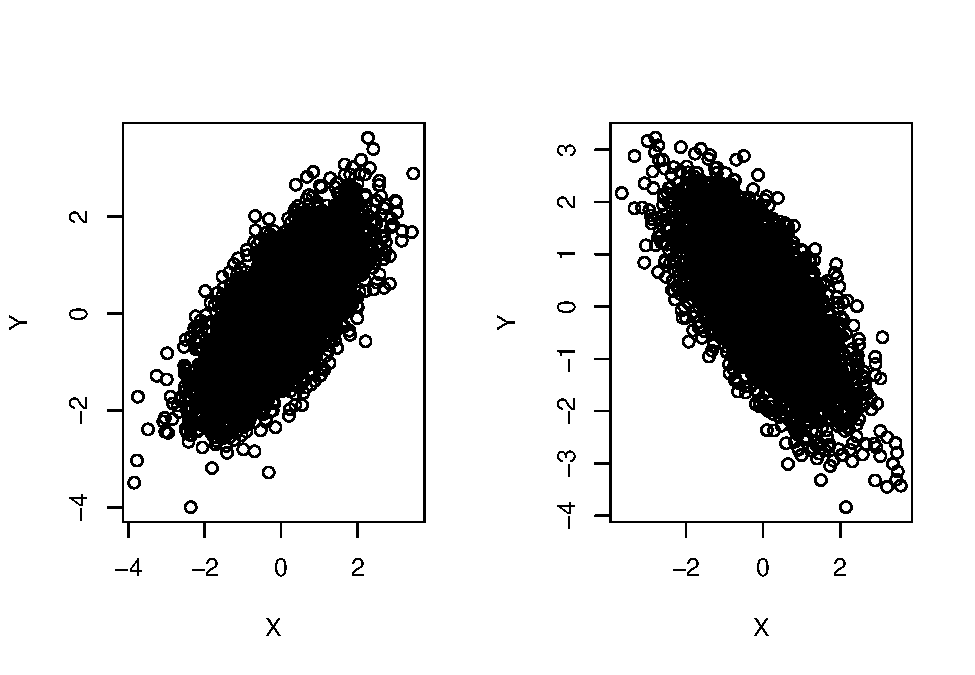
\includegraphics{bookdown-demo_files/figure-latex/5-covs-1.pdf}
\caption{\label{fig:5-covs}Positive Covariance (Left), Negative Covariance (Right)}
\end{figure}

One more thing to note: covariance and correlations can be calculated for random variables as long as they are quantitative, but not if at least one of them is categorical. The concept of increasing a random variable that is categorical does not make intuitive sense, for example, if we have a random variable that denotes the color of eyes, what does increasing color of eyes mean?

\subsection{Covariance}\label{5-cov}

We now define covariance. The \textbf{covariance} between random variables \(X\) and \(Y\) is

\begin{equation} 
Cov(X,Y) = E\left[(X- \mu_X)(Y - \mu_Y) \right].
\label{eq:5-cov}
\end{equation}

Looking at equation \eqref{eq:5-cov}, we see that if both \(X\) and \(Y\) generally move in the same direction, then \(X - \mu_x\) and \(Y - \mu_y\) will either be both positive or both negative, therefore their product is positive, on average. If \(X\) and \(Y\) generally move in opposite directions, then \(X - \mu_x\) and \(Y - \mu_y\) have opposite signs, therefore their product is negative, on average.

Some key properties for covariance:

\begin{itemize}
\tightlist
\item
  \(Cov(X,X) = Var(X)\).The covariance of any random variable with itself is its variance.
\item
  \(Cov(X,Y) = Cov(Y,X)\). The covariance between \(X\) and \(Y\) is the same as the covariance between \(Y\) and \(X\).
\item
  \(Cov(X,c) = 0\) for any constant \(c\). Since a constant does not move, it has no relationship with \(X\).
\item
  \(Cov(aX,Y) = a Cov(X,Y)\) for any constant \(a\). This implies that covariance is affected by the units of \(X\) and \(Y\).
\item
  \(Var(X + Y) = Var(X) + Var(Y) + 2 Cov(X,Y)\).
\item
  If \(X\) and \(Y\) are independent, then \(Cov(X,Y) = 0\).
\item
  However, \(Cov(X,Y) = 0\) does not mean that \(X\) and \(Y\) are independent. This is a common misconception. Remember that covariance measures linear relationship. The relationship between \(X\) and \(Y\) could be non linear, and in such instances, the covariance should not be used. Figure \ref{fig:5-cov0} below provides an example this. In this figure, \(X\) and \(Y\) have a quadratic relationship, so they are clearly not independent, yet their covariance is virtually 0.
\end{itemize}

\begin{Shaded}
\begin{Highlighting}[]
\NormalTok{x}\OtherTok{\textless{}{-}}\FunctionTok{seq}\NormalTok{(}\SpecialCharTok{{-}}\DecValTok{1}\NormalTok{,}\DecValTok{1}\NormalTok{, }\AttributeTok{by=}\FloatTok{0.01}\NormalTok{)}
\NormalTok{y}\OtherTok{\textless{}{-}}\NormalTok{x}\SpecialCharTok{\^{}}\DecValTok{2}

\DocumentationTok{\#\#note from plot that X \& Y do not have a linear relationship}
\FunctionTok{plot}\NormalTok{(x,y, }\AttributeTok{xlab=}\StringTok{"X"}\NormalTok{, }\AttributeTok{ylab=}\StringTok{"Y"}\NormalTok{)}
\end{Highlighting}
\end{Shaded}

\begin{figure}
\centering
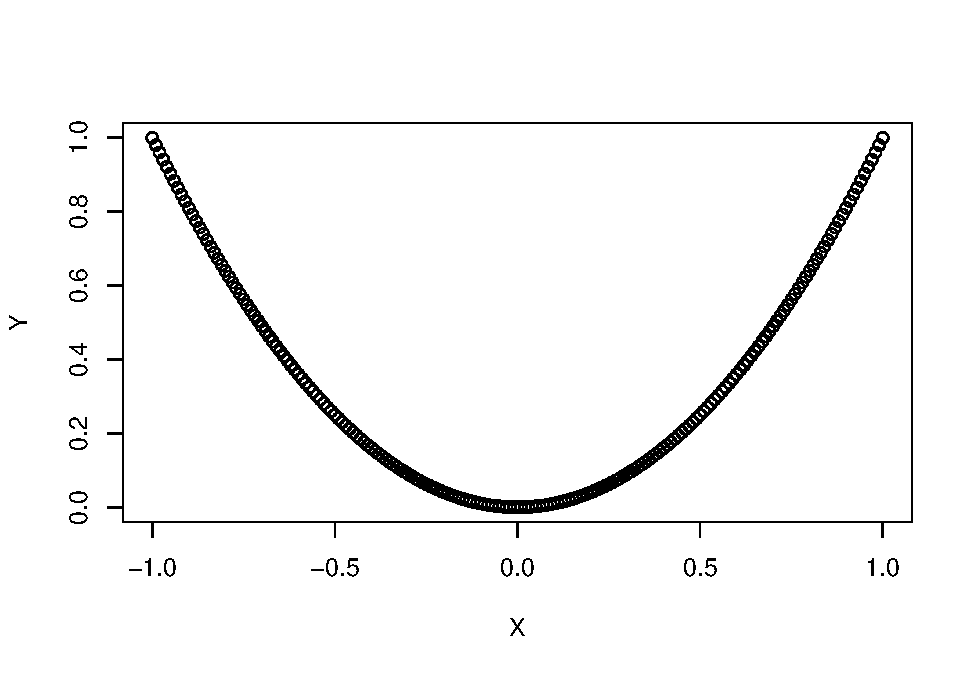
\includegraphics{bookdown-demo_files/figure-latex/5-cov0-1.pdf}
\caption{\label{fig:5-cov0}Covariance with Non Linear Relationship}
\end{figure}

\begin{Shaded}
\begin{Highlighting}[]
\FunctionTok{cov}\NormalTok{(x,y) }\DocumentationTok{\#\#covariance is virtually 0}
\end{Highlighting}
\end{Shaded}

\begin{verbatim}
## [1] 1.19967e-17
\end{verbatim}

Suppose we have two vectors of observed data, each of size \(n\): \(X = (x_1, x_2, \cdots, x_n)\) and \(Y = (y_1, y_2, \cdots, y_n)\). Their \textbf{sample covariance} is

\begin{equation} 
s_{x,y} = \frac{\sum_{i=1}^n (x_i - \bar{x})(y_i - \bar{y})}{n-1}
\label{eq:5-sampcov}
\end{equation}

We noted earlier that covariance is affected by the units of the variables. Suppose one variable is measured in meters, and we convert it to become centimeters. The value of the covariance will get multiplied by 100. People find it easier to interpret a measure that does not depend on the units. This is where the correlation comes in: it is a unitless version of the covariance.

\subsection{Correlation}\label{correlation}

The \textbf{correlation} between random variables \(X\) and \(Y\) is

\begin{equation} 
\rho = Corr(X,Y) = \frac{Cov(X,Y)}{\sqrt{Var(X) Var(Y)}}.
\label{eq:5-corr}
\end{equation}

The \textbf{sample correlation} for two vectors of observed data, each of size \(n\): \(X = (x_1, x_2, \cdots, x_n)\) and \(Y = (y_1, y_2, \cdots, y_n)\), is

\begin{equation} 
r = \frac{\sum_{i=1}^n (x_i - \bar{x})(y_i - \bar{y})}{\sqrt{\sum_{i=1}^n (x_i - \bar{x})^2 \sum_{i=1}^n (y_i - \bar{y})^2}}
\label{eq:5-sampcorr}
\end{equation}

Some key properties of correlation:

\begin{itemize}
\tightlist
\item
  It is bounded between -1 and 1.
\item
  Values closer to -1 or 1 indicate a stronger linear relationship.
\item
  Values closer to 0 indicate a weaker linear relationship.
\item
  Its numerical value is unchanged with location and / or scale changes.
\item
  If \(X\) and \(Y\) are independent, then \(Corr(X,Y) = 0\).
\item
  However, \(Corr(X,Y) = 0\) does not mean that \(X\) and \(Y\) are independent.
\item
  Correlation should only be used if the relationship between \(X\) and \(Y\) is linear.
\end{itemize}

Figure \ref{fig:5-corrs} below shows examples of some scatterplots and their sample correlations. For the left plot, the data points fall close to a straight line, is negative, and so its correlation is close to -1. The middle plot has no linear relationship, so we do not see a trend with one variable increasing or decreasing as the other variable increases. The right plot shows the data points being fairly close to a straight line, but not as close as the left plot), so its correlation is not as close to 1 (or -1).

\begin{figure}
\centering
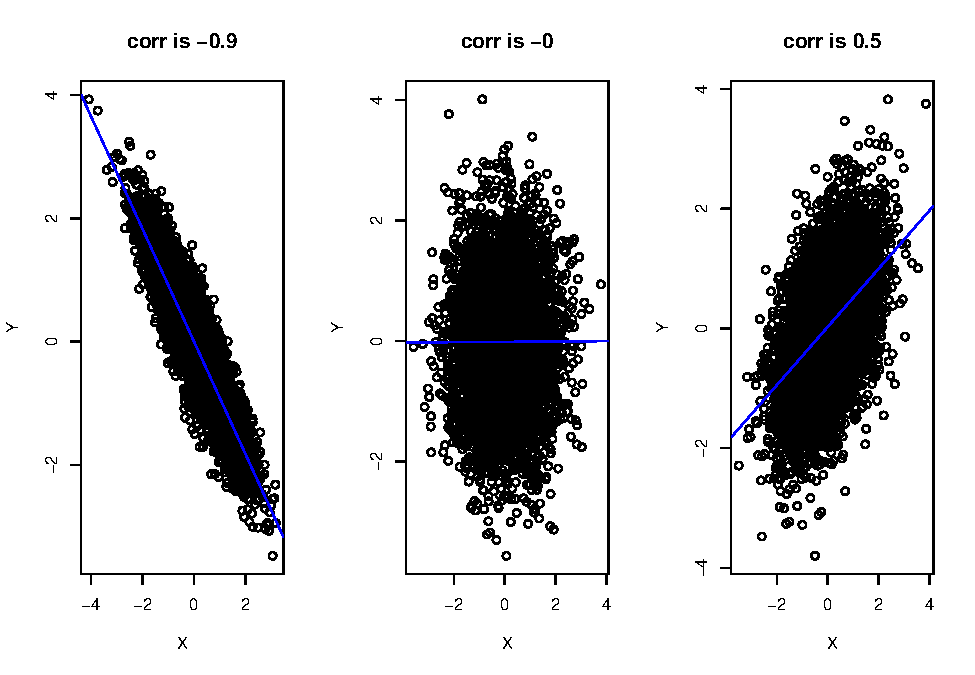
\includegraphics{bookdown-demo_files/figure-latex/5-corrs-1.pdf}
\caption{\label{fig:5-corrs}Strong Negative Correlation (Left), No Correlation (Middle), Moderate Positive Correlation (Right)}
\end{figure}

\section{Conditional Expectation}\label{conditional-expectation}

In Section \ref{condprob} and \ref{conddist}, we explored the notion of conditional probabilities and conditional distributions, whcih are used for:

\begin{itemize}
\tightlist
\item
  Updating the probability and distribution of a random variable \(Y\), after observing a certain outcome of another random variable \(X\), or
\item
  Restricting the probability and distribution of a random variable \(Y\) to a certain value of another random variable.
\end{itemize}

These represent the Bayesian and frequentist viewpoints of conditional probability and conditional distribution.

It turns out a similar idea applies to the expected value of a random variable. Recall that the expected value of a random variable is the long-run average, in other words, the average value after observing the random variable an infinite number of times.

The conditional expectation of a random variable is its long run-average:

\begin{itemize}
\tightlist
\item
  after observing a certain outcome of another variable or event, or
\item
  after restricting our attention to cases when another random variable is fixed or equal to a specific value.
\end{itemize}

Fairly often, we use statistical models to predict a response variable \(Y\) based on a predictor \(X\). Predictions for values of \(Y\) based on observed values of \(X\) usually use the conditional expectation of \(Y\) given \(X\). Given what we see with the predictor, the long run average of \(Y\) ends up being used as the predicted value of the response variable. This is the basis for most statistical models.

There are two slightly different notions of conditional expectations:

\begin{itemize}
\tightlist
\item
  Conditional expectation of random variable \(Y\) given event \(A\). If \(A\) has happened, what is the expected value of \(Y\)?
\item
  Conditional expectation of random variable \(Y\) given another random variable \(X\). If we fix the value of the random variable \(X\) to any value on its support, what is the expected value of \(Y\)?
\end{itemize}

The second notion is the one that is usually used for statistical models, but we will cover both as the first notion is easier to understand, and should help us understand the second notion.

\subsection{Conditional Expectation Given Event}\label{conditional-expectation-given-event}

Recall that the expectation \(E(Y)\) of a random variable \(Y\) is its long-run average. If \(Y\) is discrete, we take a weighted average involving the probabilities in its PMF \(P(Y=y)\). The calculation of the \textbf{conditional expectation} \(E(Y|A)\) where \(A\) is an event that has occurred simply replaces the probabilities \(P(Y=y)\) with conditional probabilities \(P(Y=y|A)\). Therefore, for a discrete random variable \(Y\),

\begin{equation} 
E(Y|A) = \sum_y y P(Y=y|A) 
\label{eq:5-condexpdis}
\end{equation}

where the sum is over the support of \(Y\). Notice how we are summing the product of the support with its corresponding conditional probability, whereas to find \(E(Y)\), we sum the product of the support with its corresponding unconditional probability.

If \(Y\) is continuous, we use the conditional PDF instead:

\begin{equation} 
E(Y|A) = \int_{-\infty}^{\infty} y f(y|A) dy.
\label{eq:5-condexpcont}
\end{equation}

The key is to understand the intuition behind conditional expectations, and we will use simulation to approximate this (the approximation works better if we use more simulated data). Simulation represents the frequentist viewpoint of conditional expectation. The code below does the following:

\begin{itemize}
\tightlist
\item
  Generate 100 values of \(X\) uniformly on the support \(\{1,2,3,4\}\).
\item
  Simulate \(Y\) using \(Y = 10 + X + \epsilon\) where \(\epsilon \sim N(0,1)\).
\item
  Represent these values on a scatter plot, and also overlay a line that represents the sample mean of \(Y\), which estimates \(E(Y)\). This is simply the average value on the y-axis for all 100 data points. This is the plot on the left in Figure \ref{fig:5-condexp} below.
\item
  Represent these values on a scatter plot, but use blue to denote the event \(A\) which is when \(X=1\). A line that represents the sample mean of \(Y\), only for these blue data points (i.e.~only when \(X=1\)), is overlaid. This value estimates \(E(Y|A)\) or \(E(Y|X=1)\). This is the plot on the right in Figure \ref{fig:5-condexp} below. In calculating this sample mean, we could have completed disregarded the black data points when \(X\) was not 1.
\end{itemize}

\begin{Shaded}
\begin{Highlighting}[]
\FunctionTok{set.seed}\NormalTok{(}\DecValTok{40}\NormalTok{)}
\NormalTok{n}\OtherTok{\textless{}{-}}\DecValTok{100} \DocumentationTok{\#\#100 data points}

\DocumentationTok{\#\#generate X}
\NormalTok{x}\OtherTok{\textless{}{-}}\FunctionTok{c}\NormalTok{(}\FunctionTok{rep}\NormalTok{(}\DecValTok{1}\NormalTok{,n}\SpecialCharTok{/}\DecValTok{4}\NormalTok{), }\FunctionTok{rep}\NormalTok{(}\DecValTok{2}\NormalTok{,n}\SpecialCharTok{/}\DecValTok{4}\NormalTok{), }\FunctionTok{rep}\NormalTok{(}\DecValTok{3}\NormalTok{,n}\SpecialCharTok{/}\DecValTok{4}\NormalTok{), }\FunctionTok{rep}\NormalTok{(}\DecValTok{4}\NormalTok{,n}\SpecialCharTok{/}\DecValTok{4}\NormalTok{)) }

\DocumentationTok{\#\#simulate Y}
\NormalTok{y}\OtherTok{\textless{}{-}} \DecValTok{10} \SpecialCharTok{+}\NormalTok{ x }\SpecialCharTok{+} \FunctionTok{rnorm}\NormalTok{(n)}

\FunctionTok{par}\NormalTok{(}\AttributeTok{mfrow=}\FunctionTok{c}\NormalTok{(}\DecValTok{1}\NormalTok{,}\DecValTok{2}\NormalTok{))}
\FunctionTok{plot}\NormalTok{(x,y, }\AttributeTok{main=}\StringTok{"Estimated E(Y) Overlaid"}\NormalTok{)}
\FunctionTok{abline}\NormalTok{(}\AttributeTok{h=}\FunctionTok{mean}\NormalTok{(y)) }\DocumentationTok{\#\#add line to represent est E(Y)}

\FunctionTok{plot}\NormalTok{(x,y, }\AttributeTok{col =} \FunctionTok{ifelse}\NormalTok{(x }\SpecialCharTok{==} \DecValTok{1}\NormalTok{,}\StringTok{\textquotesingle{}blue\textquotesingle{}}\NormalTok{, }\StringTok{\textquotesingle{}black\textquotesingle{}}\NormalTok{), }\AttributeTok{pch =} \DecValTok{19}\NormalTok{, }\AttributeTok{main=}\StringTok{"Estimated E(Y|X=1) Overlaid"}\NormalTok{ )}
\FunctionTok{abline}\NormalTok{(}\AttributeTok{h=}\FunctionTok{mean}\NormalTok{(y[}\AttributeTok{x=}\DecValTok{1}\NormalTok{]), }\AttributeTok{col=}\StringTok{"blue"}\NormalTok{) }\DocumentationTok{\#\#add line to represent est E(Y|X=1)}
\end{Highlighting}
\end{Shaded}

\begin{figure}
\centering
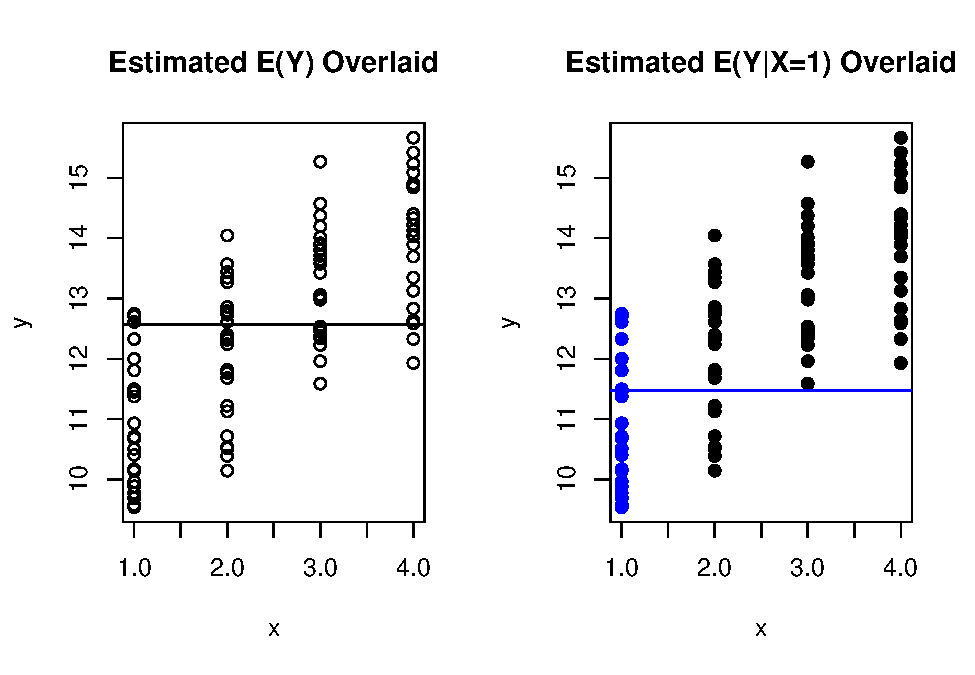
\includegraphics{bookdown-demo_files/figure-latex/5-condexp-1.pdf}
\caption{\label{fig:5-condexp}Comparison of E(Y) and E(Y\textbar X=1)}
\end{figure}

So, we can interpret the conditional expectation \(E(Y|A)\) as the long-run average of \(Y\) (only) when \(A\) has happened. It is the long-run average of \(Y\) when a certain condition is met.

\subsection{Conditional Expectation Given Random Variable}\label{conditional-expectation-given-random-variable}

The conditional expectation of \(Y\) given a random variable \(X\) is slightly different. In the simulated example in the previous subsection, we set \(X\) to be a specific value. Now, we consider the long-run average of \(Y\) for each value, instead of a specific value, in the support of \(X\).

One way to think about this is to consider \(E(Y|X=x)\), where \(x\) is any value on the support for \(X\). If \(Y\) is discrete, this conditional expectation is:

\begin{equation} 
E(Y|A) = \sum_y y P(Y=y|X=x) 
\label{eq:5-condexpdis2}
\end{equation}

where the sum is over the support of \(Y\).

If \(Y\) is continuous:

\begin{equation} 
E(Y|A) = \int_{-\infty}^{\infty} y f(y|x) dy.
\label{eq:5-condexpcont2}
\end{equation}

We go back to the simulated example in the previous subsection to explain what \(E(Y|X=x)\) represents. Recall that the support for \(X\) is \(\{1,2,3,4\}\) and that \(Y = 10 + X + \epsilon\) where \(\epsilon \sim N(0,1)\). So

\[
\begin{split}
E(Y|X=x) &= E(10 + X + \epsilon | X=x)\\
 &= E(10 + x + \epsilon) \\
 &= E(10) + E(x) + E(\epsilon) \\
&= 10 + x + 0 \\
 &= 10 + x.
\end{split}
\]

A brief explanation of each step:

\begin{itemize}
\tightlist
\item
  To go from line 1 to line 2, we subbed in \(x\) for \(X\), since we are setting \(X=x\).
\item
  To go from line 2 to line 3, we apply the linearity of expectations.
\item
  To go from line 3 to 4, \(E(c)=c\) for any constant. In this case, we are fixing \(x\) to be a value in the support so it is a constant, and \(E(\epsilon) = 0\) since \(\epsilon \sim N(0,1)\).
\end{itemize}

So \(E(Y|X) = 10 + X\). What this means is that:

\begin{itemize}
\tightlist
\item
  When \(X=1\), \(E(Y|X=1) = 11\),
\item
  When \(X=2\), \(E(Y|X=1) = 12\),
\item
  When \(X=3\), \(E(Y|X=1) = 13\), and
\item
  When \(X=4\), \(E(Y|X=1) = 14\).
\end{itemize}

Note: We set up \(Y = 10 + X + \epsilon\) where \(\epsilon \sim N(0,1)\) in the simulation. This follows the framework for linear regression which sets up \(Y = \beta_0 + \beta_1 X + \epsilon\) where \(\epsilon \sim N(0,\sigma^2)\), i.e.~\(\epsilon\) is normal with mean 0 and a variance that is a fixed value. The conditional expectation given \(X\) ends up being the prediction for \(Y\) that minimizes the mean squared error in linear regression.

\section{Common Multivariate Distributions}\label{common-multivariate-distributions}

We now cover two of the most common multivariate distributions: the multinomial distribution and multivariate normal distribution for discrete and continuous random variables respectively.

\subsection{Multinomial}\label{multinomial}

The \textbf{multinomial} distribution can be viewed as a generalization of the binomial distribution into higher dimensions. Recall that for the binomial distribution, we carry out \(n\) trials, and for each trial we record whether it as a success or failure, in other words, there are only two outcomes for each trial. The multinomial distribution differs in that there can be more than two outcomes for each trial. For example, we randomly select \(n\) adults and ask them for their political affiliation. The affiliation could be Democrat, Republican, other party, or no affiliation, so there are four possible outcomes or categories for each person.

The set up of the multinomial distribution is as follows:

\begin{itemize}
\tightlist
\item
  We have \(n\) independent trials, and each trial belongs to one of \(k\) categories.
\item
  Each trial belongs to category \(j\) with probability \(p_j\), where \(p_j\) is non negative and \(\sum_{j=1}^k p_j = 1\), i.e.~they sum to one.
\item
  Let \(X_1\) denote the number of trials belonging to category 1, \(X_2\) denote the number of trials belonging to category 2, and so on. Then \(X_1 + \cdots X_k = n\).
\end{itemize}

We then say that \(\boldsymbol{X} = (X_1, \cdots, X_k)\) is said to have a multinomial distribution with parameters \(n\) and \(\boldsymbol{p} = (p_1, \cdots, p_k)\). This can be written as \(\boldsymbol{X} \sim Mult_k(n, \boldsymbol{p})\).

Note that the vectors \(\boldsymbol{X}\) and \(\boldsymbol{p}\) are written in bold. Vectors and matrices are commonly written using bold to distinguish them from scalars, which are not in bold. \(\boldsymbol{X}\) is an example of what we call a random vector, as it is a vector of random variables \(X_1, \cdots, X_k\).

If \(\boldsymbol{X} \sim Mult_k(n, \boldsymbol{p})\), its PMF is

\begin{equation} 
P(X_1 = n_1, \cdots, X_k = n_k) = \frac{n!}{n_{1}! \cdots n_{k}!} p_1^{n_1} \cdots p_k^{n_k},
\label{eq:5-multinomial}
\end{equation}

where \(n_1 + \cdots + n_k = n\).

Let us use a toy example. Going back to political affiliations. Suppose among American voters, 28\% identify as Democrats, 29\% identify as Republicans, and 10\% identify have other affiliations, and 33\% are independents. Let \(X_1, X_2, X_3, X_4\) denote the number of Democrats, Republicans, others, and independents. The joint distribution of \(X_1, X_2, X_3, X_4\) is \(\boldsymbol{X} = (X_1, X_2, X_3, X_4) \sim Mult_4(0.28, 0.29, 0.1, 0.33)\).

Suppose we want to find the probability that in a sample of 10 voters, 2 are Democrats, 3 are Republicans, and 1 has another affiliation, and 4 are Independents:

\[
\begin{split}
P(X_1 = 2, X_2 = 3, X_3 = 1, X_4 = 4) &= \frac{10!}{2! 3! 1!4!} 0.28^{2} 0.29^{3} 0.1^1 0.33^4\\
 &= 0.02857172.
\end{split}
\]

Or use

\begin{Shaded}
\begin{Highlighting}[]
\FunctionTok{dmultinom}\NormalTok{(}\FunctionTok{c}\NormalTok{(}\DecValTok{2}\NormalTok{,}\DecValTok{3}\NormalTok{,}\DecValTok{1}\NormalTok{,}\DecValTok{4}\NormalTok{), }\AttributeTok{prob=}\FunctionTok{c}\NormalTok{(}\FloatTok{0.28}\NormalTok{,}\FloatTok{0.29}\NormalTok{,}\FloatTok{0.1}\NormalTok{,}\FloatTok{0.33}\NormalTok{)) }\DocumentationTok{\#\#specify X1, X2, X3, X4, then p1,p2,p3, p4}
\end{Highlighting}
\end{Shaded}

\begin{verbatim}
## [1] 0.02857172
\end{verbatim}

\subsubsection{Multinomial Marginals}\label{multinomial-marginals}

The marginals of a multinomial are binomial. For \(\boldsymbol{X} \sim Mult_k(n, \boldsymbol{p})\), \(X_j \sim Bin(n, p_j)\).

Going back to our toy example with American voters, this means that \(X_1 \sim Bin(n,0.28), X_2 \sim Bin(n,0.29), X_3 \sim Bin(n, 0.1), X_4 \sim Bin(n,0.33)\). Hopefully this example makes sense. If we look at \(X_1,\) we are looking at the number of voters who are democrats and those who are not. The proportion of Democrats still remains the same, while the proportion of Republicans, other affiliations, and independents is the sum of their individual proportions, or 1 minus the proportion of Democrats.

\subsubsection{Multinomial Lumping}\label{multinomial-lumping}

With discrete and categorical variables, it can be common to want to lump (or merge, or collapse, or combine) categories together. If \(\boldsymbol{X} \sim Mult_k(n, \boldsymbol{p})\), then \(X_i + X_j \sim Bin(n, p_i + p_j)\). If we decide to merge categories 1 and 2, we have \((X_1 + X_2, X_3, \cdots, X_k) \sim Mult_{k-1}(n, (p_1 + p_2, p_3, \cdots, p_k))\).

We go back to our toy example. Suppose we consider Democrats and Republicans to be the major parties, we may wish to combine everyone else into one category: those with other affiliations and independents. We can define this using a new random variable \(\boldsymbol{Y} = (X_1, X_2, X_3+X_4) \sim Mult_3(n,(0.29,0.29,0.43)\). Note we now have 3 categories instead of 4. The proportion for the lumped category is the sum of their individual proportions.

\subsubsection{Multinomial Covariance}\label{multinomial-covariance}

For \(\boldsymbol{X} \sim Mult_k(n, \boldsymbol{p})\) with \(\boldsymbol{p} = (p_1,p_2, \cdots, p_k)\). The covariance between any two distinct components \(X_i\) and \(X_j\) is

\begin{equation} 
Cov(X_i, X_j) = -n p_i p_j,
\label{eq:5-multinomialcov}
\end{equation}

for any \(i \neq j\). The book provides a nice proof, under Theorem 7.4.6, for those interested.

Looking at \eqref{eq:5-multinomialcov}, we notice the covariance between any two distinct components is negative (since probabilities are non negative). This means that the numerical values of \(X_i\) and \(X_j\) go in opposite directions. This should make intuitive sense since \(n = X_1 + \cdots + X_k\) is fixed, so if \(X_i\) is large, \(X_j\) should be small since \(n\) is fixed. An extreme example will be if \(X_i = n\), then \(X_j\) must be 0.

We go back to our toy example. Suppose we want to find the correlation between \(X_1\) and \(X_2\), the number of Democrats and Republicans in a sample of size \(n\). Note that \(X_1 \sim Bin(n,0.28), X_2 \sim Bin(n,0.29)\), and \(Cov(X_1,X_2) = -n \times 0.28 \times 0.29 = 0.0812n\),

\[
\begin{split}
Corr(X_1,X_2) &= \frac{Cov(X_1,X_2)}{\sqrt{Var(X_1) Var(X_2)}}\\
 &= \frac{-n p_1 p_2}{\sqrt{n p_1 (1-p_1) n p_2 (1-p_2)}} \\
 &= -\sqrt{\frac{p_1 p_2}{(1-p_1)(1-p_2)}} \\
 &= -\sqrt{\frac{0.28 \times 0.29}{(1-0.28)(1-0.29)}} \\
 &= -0.3985498.
\end{split}
\]

\subsubsection{Conditional Multinomial}\label{conditional-multinomial}

Sometimes, we have some observed data from a multinomial distribution, and wish to update the distribution. Suppose we have \(\boldsymbol{X} \sim Mult_k(n, \boldsymbol{p})\), and we observed that \(X_1 = n_1\), then \((X_2, \cdots, X_k)|X_1 = n_1 \sim Mult_{k-1}(n-n_1, (p_2^{\prime}, \cdots, p_k^{\prime}))\) where \(p_j^{\prime} = \frac{p_j}{p_2 + \cdots + p_k}\).

\subsection{Multivariate Normal}\label{multivariate-normal}

The \textbf{multivariate normal} (MVN) distribution can be viewed as a generalization of the normal distribution into higher dimensions. Just like the univariate normal distribution, the central limit theorem also applies to higher dimensions.

A \(k\)-dimensional random vector \(\boldsymbol{X} = (X_1, \cdots, X_k)\) is said to have an MVN distribution if every linear combination of the \(X_j\) is normal. This means that \(t_1 X_1 + \cdots + t_k X_k\) is normally distributed for any constants \(t_1, \cdots, t_k\). When \(k=2\), the MVN is often called a \textbf{bivariate normal}.

In Section \ref{norm}, we mentioned that the parameters of a normal distribution are its mean \(\mu\) and variance \(\sigma^2\). This idea is generalized to a MVN \(\boldsymbol{X} = (X_1, \cdots, X_k)\). The parameters are:

\begin{itemize}
\item
  the \textbf{mean vector} \((\mu_1, \cdots, \mu_k)\) where \(\mu_j = E(X_j)\). This is a vector of length \(k\) where each entry is the expected value of that component.
\item
  the \textbf{covariance matrix}. This is a \(k \times k\) matrix where the \((i,j)\)th entry (i.e.~row \(i\), column \(j\)) is the covariance between \(X_i\) and \(X_j\). This implies that the diagonal entries give the variance of each component (since \(Cov(X_i, X_i) = Var(X_i)\)), and the covariance matrix is symmetric (since \(Cov(X_i, X_j) = Cov(X_j, X_i)\)).
\end{itemize}

For example, suppose we have \(\boldsymbol{X} = (X_1, X_2, X_3)\) that is MVN with mean vector \((5, 2, 8)\) and covariance matrix

\[
\begin{pmatrix}
3 & 1.5 & 2.5\\
1.5 & 2 & 4.2 \\
2.5 & 4.2 & 1
\end{pmatrix},
\]

then

\begin{itemize}
\tightlist
\item
  \(E(X_1) = 5, E(X_2) = 2, E(X_3) = 8\),
\item
  \(Var(X_1) = 3, Var(X_2) = 2, Var(X_3) = 1\),
\item
  \(Cov(X_1, X_2) = Cov(X_2, X_1) = 1.5\),
\item
  \(Cov(X_1, X_3) = Cov(X_3, X_1) = 2.5\), and
\item
  \(Cov(X_2, X_3) = Cov(X_3, X_2) = 4.2\).
\end{itemize}

Some properties of the MVN distribution:

\begin{enumerate}
\def\labelenumi{\arabic{enumi}.}
\item
  If \(\boldsymbol{X} = (X_1, \cdots, X_k)\) is MVN, the marginal distribution of each \(X_j\) is normal, as we can set \(t_j =1\) and all other constants to be 0.
\item
  However, the converse is not necessarily true. If each \(X_1, \cdots, X_k\) is normal, \((X_1, \cdots, X_k)\) is not necessarily MVN.
\item
  If \((X_1, \cdots, X_k)\) is MVN, then so is any subvector, e.g.~\((X_i, X_j)\) is bivariate normal.
\item
  If \(\boldsymbol{X} = (X_1, \cdots, X_k)\) and \(\boldsymbol{Y} = (Y_1, \cdots, Y_m)\) are MVN with \(\boldsymbol{X}\) independent of \(\boldsymbol{Y}\), then \(\boldsymbol{W} = (X_1, \cdots, X_k, Y_1, \cdots, Y_m)\) is MVN.
\item
  Within an MVN random vector, uncorrelated implies independence. If \(\boldsymbol{X}\) is MVN and \(\boldsymbol{X} = (\boldsymbol{X_1, X_2})\) where \(\boldsymbol{X_1}\) and \(\boldsymbol{X_2}\) are subvectors, and every component of \(\boldsymbol{X_1}\) is uncorrelated with every component of \(\boldsymbol{X_2}\), then \(\boldsymbol{X_1}\) and \(\boldsymbol{X_2}\) are independent.
\end{enumerate}

\subsubsection{Simulations}\label{simulations}

We can use simulations to verify the first property. For this simulation, we will do the following:

\begin{itemize}
\tightlist
\item
  Simulate 5000 draws from a MVN distribution with mean vector \((1,2,5)\) and covariance matrix
\end{itemize}

\[
\begin{pmatrix}
1 & 0.5 & 0.6\\
0.5 & 2 & 0.2 \\
0.6 & 0.2 & 4
\end{pmatrix}.
\]

\begin{itemize}
\item
  Assess if each component \(X_1, X_2, X_3\) is normally distributed by using the Shapiro-Wilk test for normality.

  \begin{itemize}
  \tightlist
  \item
    The null hypothesis is that the variable follows a normal distribution, and the alternative hypothesis is that the variable does not follow a normal distribution.
  \item
    So rejecting the null hypothesis means the variable is inconsistent with a normal distribution, while not rejecting means we do not have evidence the variable is inconsistent with a normal distribution.
  \item
    We will record the p-value of each test on \(X_1, X_2, X_3\).
  \end{itemize}
\item
  Repeat the previous 2 steps for a total of 10 thousand reps.
\item
  Count the proportion of reps where the Shapiro-Wilk test rejected the null hypothesis at significance level 0.05 for \(X_1, X_2, X_3\).

  \begin{itemize}
  \tightlist
  \item
    If this property is correct, we will expect close to 5\% of the p-values to (wrongly) reject the null hypothesis, since the tests are conducted at 0.05 significance level.
  \end{itemize}
\end{itemize}

\begin{Shaded}
\begin{Highlighting}[]
\FunctionTok{library}\NormalTok{(mvtnorm) }\DocumentationTok{\#\#package to simulate from MVN}

\NormalTok{reps}\OtherTok{\textless{}{-}}\DecValTok{1000} \DocumentationTok{\#\# how many reps}
\NormalTok{pvalsx1}\OtherTok{\textless{}{-}}\NormalTok{pvalsx2}\OtherTok{\textless{}{-}}\NormalTok{pvalsx3}\OtherTok{\textless{}{-}}\FunctionTok{array}\NormalTok{(}\DecValTok{0}\NormalTok{,reps) }\DocumentationTok{\#\#initialize an array to store the pvalues from each test at each rep}
\NormalTok{siglevel}\OtherTok{\textless{}{-}}\FloatTok{0.05} \DocumentationTok{\#\#sig level}
\NormalTok{n}\OtherTok{\textless{}{-}}\DecValTok{5000} \DocumentationTok{\#\#number of draws for each rep}

\NormalTok{mu\_vector}\OtherTok{\textless{}{-}}\FunctionTok{c}\NormalTok{(}\DecValTok{1}\NormalTok{,}\DecValTok{2}\NormalTok{,}\DecValTok{5}\NormalTok{) }\DocumentationTok{\#\#mean vector}

\DocumentationTok{\#\#set up covariance matrix}
\NormalTok{sig12}\OtherTok{\textless{}{-}}\FloatTok{0.5}
\NormalTok{sig13}\OtherTok{\textless{}{-}}\FloatTok{0.6}
\NormalTok{sig23}\OtherTok{\textless{}{-}}\FloatTok{0.2}
\NormalTok{cov\_mat}\OtherTok{\textless{}{-}}\FunctionTok{matrix}\NormalTok{(}\FunctionTok{c}\NormalTok{(}\DecValTok{1}\NormalTok{,sig12,sig13,sig12,}\DecValTok{2}\NormalTok{,sig23,sig13,sig23,}\DecValTok{4}\NormalTok{), }\AttributeTok{nrow=}\DecValTok{3}\NormalTok{, }\AttributeTok{ncol=}\DecValTok{3}\NormalTok{)}

\DocumentationTok{\#\#set.seed so you can replicate my result.}
\FunctionTok{set.seed}\NormalTok{(}\DecValTok{30}\NormalTok{)}

\DocumentationTok{\#\#run steps 1 and 2 for 10 000 times}
\ControlFlowTok{for}\NormalTok{ (i }\ControlFlowTok{in} \DecValTok{1}\SpecialCharTok{:}\NormalTok{reps)}
  
\NormalTok{\{}

\NormalTok{  data}\OtherTok{\textless{}{-}}\FunctionTok{rmvnorm}\NormalTok{(n, mu\_vector, cov\_mat)}
  
\NormalTok{  x1}\OtherTok{\textless{}{-}}\NormalTok{data[,}\DecValTok{1}\NormalTok{] }\DocumentationTok{\#\#extract X1}
\NormalTok{  x2}\OtherTok{\textless{}{-}}\NormalTok{data[,}\DecValTok{2}\NormalTok{] }\DocumentationTok{\#\#extract X2}
\NormalTok{  x3}\OtherTok{\textless{}{-}}\NormalTok{data[,}\DecValTok{3}\NormalTok{] }\DocumentationTok{\#\#extract X3}
  
  \DocumentationTok{\#\#store pvalue from Shapiro{-}Wilk test from each component}
\NormalTok{  pvalsx1[i]}\OtherTok{\textless{}{-}}\FunctionTok{shapiro.test}\NormalTok{(x1)}\SpecialCharTok{$}\NormalTok{p.value }
\NormalTok{  pvalsx2[i]}\OtherTok{\textless{}{-}}\FunctionTok{shapiro.test}\NormalTok{(x2)}\SpecialCharTok{$}\NormalTok{p.value}
\NormalTok{  pvalsx3[i]}\OtherTok{\textless{}{-}}\FunctionTok{shapiro.test}\NormalTok{(x3)}\SpecialCharTok{$}\NormalTok{p.value }
  
\NormalTok{\}}

\DocumentationTok{\#\#proportion of tests that wrongly reject the null}
\FunctionTok{sum}\NormalTok{(pvalsx1}\SpecialCharTok{\textless{}}\NormalTok{siglevel)}\SpecialCharTok{/}\NormalTok{reps }\DocumentationTok{\#\#for X1}
\end{Highlighting}
\end{Shaded}

\begin{verbatim}
## [1] 0.054
\end{verbatim}

\begin{Shaded}
\begin{Highlighting}[]
\FunctionTok{sum}\NormalTok{(pvalsx2}\SpecialCharTok{\textless{}}\NormalTok{siglevel)}\SpecialCharTok{/}\NormalTok{reps }\DocumentationTok{\#\#for X2}
\end{Highlighting}
\end{Shaded}

\begin{verbatim}
## [1] 0.037
\end{verbatim}

\begin{Shaded}
\begin{Highlighting}[]
\FunctionTok{sum}\NormalTok{(pvalsx3}\SpecialCharTok{\textless{}}\NormalTok{siglevel)}\SpecialCharTok{/}\NormalTok{reps }\DocumentationTok{\#\#for X3}
\end{Highlighting}
\end{Shaded}

\begin{verbatim}
## [1] 0.047
\end{verbatim}

Since close to 5\% of each hypothesis test rejected the null hypothesis, it appears that each component is consistent with a normal distribution. (Or more accurately, we do not have evidence to say that each component is not normal.) It does appear that if \(\boldsymbol{X} = (X_1, \cdots, X_k)\) is MVN, the marginal distribution of each \(X_j\) is normal. Our simulation does not provide evidence against this property.

Note: What we have done is called a Monte Carlo simulation, and is often used in research to verify theorems. While you may not be involved in research, writing code to run simulations is a good way for you to understand these theorems and how they are applied. We will cover Monte Carlo simulations in more detail in a later module.

\chapter{Inequalities, Limit Theorems, and Simulations}\label{inequalities-limit-theorems-and-simulations}

This module is based on Introduction to Probability (Blitzstein, Hwang), Chapter 10. You can access the book for free at \url{https://stat110.hsites.harvard.edu/} (and then click on Book). Please note that I cover additional topics, and skip certain topics from the book. You may skip Eample 10.1.3, 10.1.4, 10.1.7 to 10.1.9, Theorem 10.1.12, Example 10.2.5, 10.2.6, 10.3.7, and Section 10.4 from the book.

\section{Introduction}\label{introduction-2}

It can be difficult to calculate probabilities and expected values, for example, when the PDF of a distribution is unknown, or its integral is too difficult to work out. You may notice that we used simulations to approximate probabilities and expected values in some of the examples in previous modules. With improvement in computing capabilities, simulations can now be performed faster and is a tool that is used more and more. Other tools include using inequalities to bound the probabilities (e.g.~the probability cannot be greater or less than a certain value), or approximating using known theorems. We'll look at these three tools in this module.

\section{Inequalities}\label{inequalities}

If a probability or expected value is difficult to calculate, it may be easier to find a bound via an inequality. This usually means that we can guarantee that a certain probability or expected value is within a certain range of values, so we can narrow down the possible values for the exact answer. For example, instead of being able to calculate the probability of a certain event, we may be able to show that its probability is no more than 0.1, so we know the event is unlikely to happen. We will cover a couple of the most well-known inequalities in probability.

\subsection{Cauchy-Schwartz Inequality}\label{cauchy-schwartz-inequality}

The \textbf{Cauchy-Schwarz inequality} is one of the most famous inequalities in mathematics and has many applications. In the context of probability, it is written as: For any random variables \(X\) and \(Y\) with finite variances

\begin{equation} 
|E(XY)| \leq \sqrt{E(X^2)E(Y^2)}.
\label{eq:6-CS}
\end{equation}

Next, we use the Cauchy-Schwartz inequality to prove a couple of properties that we have stated in earlier modules:

\begin{enumerate}
\def\labelenumi{\arabic{enumi}.}
\tightlist
\item
  The Cauchy-Schwartz inequality can be used to show the correlation between any two random variables with finite variances must be between -1 and 1. A quick proof is as follows: we apply equation \eqref{eq:6-CS} to the \textbf{centered} random variables \(X - \mu_X\) and \(Y - \mu_Y\):
\end{enumerate}

\[
\begin{split}
|E[(X - \mu_X)(Y - \mu_Y)]| & \leq \sqrt{E[(X - \mu_X)^2] E[(Y - \mu_Y)^2]} \\
\implies |Cov(X,Y)| & \leq \sqrt{Var(X) Var(Y)} \\
\implies |Corr(X,Y)| & \leq 1.
\end{split}
\]

\begin{enumerate}
\def\labelenumi{\arabic{enumi}.}
\setcounter{enumi}{1}
\tightlist
\item
  The Cauchy-Schwarz inequality can also be used to show that the variance of any random variable has to be non negative. A quick proof is as follows: we apply equation \eqref{eq:6-CS} to the random variable \(X\) and to a constant 1:
\end{enumerate}

\[
\begin{split}
|E(X)| & \leq \sqrt{E(X^2)E(1^2)}. \\
\implies |E(X)| & \leq \sqrt{E(X^2)} \\
\implies E(X)^2 & \leq E(X^2) \\
\implies 0 & \leq E(X^2) - E(X)^2 = Var(X).
\end{split}
\]
Note: One other place that you may seen the Cauchy-Schwarz inequality is in the proof of the triangle inequality in geometry.

\subsection{Jensen's Inequality}\label{jensens-inequality}

You may have noticed in previous modules, we have written about transforming a random variable. One way of transforming a random variable is through a scale change, in other words, the value of the random variable is multiplied by a constant. This happens when we change the units of the variable. For example we want to convert a random variable based on weight from kilograms to pounds. If \(X\) and \(Y\) denote the weight in kilograms and pounds respectively, we can write \(Y = 2.2X\). If we know the expected value of \(X\), we can easily find the expected value for \(Y\) by multiplying \(E(X)\) by 2.2. This is fairly intuitive and is based on the linearity of expectations using equation \eqref{eq:3-linEX}.

Before stating Jensen's inequality, we have to cover a couple of concepts: linear vs non linear transformations, and convex vs concave functions.

\subsubsection{Linear and Non Linear Transformations}\label{linnonlin}

A way to think about transformations is to write \(Y = g(X)\), where \(g\) is a function that describes the transformation. In the kilograms to pounds example, \(g\) is exactly 2.2, so \(Y = 2.2X\). This transformation is a \textbf{linear transformation} since the graph of \(Y = 2.2X\) is a straight line. In this example, \(E(Y) = E(2.2X) = 2.2E(X)\).

What if we use a \textbf{non linear transformation}? A popular non linear transformation is a log transformation. This is used when a random variable is right skewed (which happens pretty often in real data, such as wages, since only a few people make really high wages and the vast majority of people have wages on the lower end). Expected values are often used in statistical models for predictions; however, we know that the mean may not be the best measure of centrality with skewed data. One way to transform right skewed data to become less skewed is to log transform the data. In this example, we have \(Y = \log(X)\), so \(g(x) = \log(x)\). If we know the expected value of the original variable, \(E(X)\), can we easily find the expected value of \(Y\)? Can we write \(E(Y) = E(\log(X)) = \log E(X)\)? This is actually incorrect. It turns out that such operations do not work for non linear transformations, i.e.~if \(g\) is non linear, \(E(g(X))\) is not necessarily equal to \(g(E(X))\). A log transformation is not linear since the graph of \(Y = \log(X)\) is not a straight line.

Let us use a toy example to show this. Suppose we roll a fair six-sided die, and let \(X\) denote the number of dots the die shows. For this game, we get to win money based on the result of the roll, specifically twice the result. Let \(D\) denote the winnings for this game, so \(D = 2X\). Since we know \(E(X) = 3.5\), this means that the expected winnings for this game is \(E(D) = E(2X) = 2E(X) = 7\), since we have linear transformation here. The code below verifies these:

\begin{Shaded}
\begin{Highlighting}[]
\NormalTok{X}\OtherTok{\textless{}{-}}\FunctionTok{c}\NormalTok{(}\DecValTok{1}\NormalTok{,}\DecValTok{2}\NormalTok{,}\DecValTok{3}\NormalTok{,}\DecValTok{4}\NormalTok{,}\DecValTok{5}\NormalTok{,}\DecValTok{6}\NormalTok{) }\DocumentationTok{\#\#support for X}

\NormalTok{D}\OtherTok{\textless{}{-}}\DecValTok{2}\SpecialCharTok{*}\NormalTok{ X }\DocumentationTok{\#\#winnings}

\FunctionTok{mean}\NormalTok{(X) }\DocumentationTok{\#\#EX since die is fair}
\end{Highlighting}
\end{Shaded}

\begin{verbatim}
## [1] 3.5
\end{verbatim}

\begin{Shaded}
\begin{Highlighting}[]
\FunctionTok{mean}\NormalTok{(D) }\DocumentationTok{\#\#Expected winnings. This is equal to 2 times mean(X)}
\end{Highlighting}
\end{Shaded}

\begin{verbatim}
## [1] 7
\end{verbatim}

Now suppose the winnings is now defined as the squared of the number of dots the die shows. Let \(T\) denote the new winnings, so \(T = X^2\). Since this is a non linear transformation, \(E(T) = E(X^2)\) may not equal to \(E(X)^2\):

\begin{Shaded}
\begin{Highlighting}[]
\NormalTok{X}\OtherTok{\textless{}{-}}\FunctionTok{c}\NormalTok{(}\DecValTok{1}\NormalTok{,}\DecValTok{2}\NormalTok{,}\DecValTok{3}\NormalTok{,}\DecValTok{4}\NormalTok{,}\DecValTok{5}\NormalTok{,}\DecValTok{6}\NormalTok{) }\DocumentationTok{\#\#support for X}

\NormalTok{T}\OtherTok{\textless{}{-}}\NormalTok{X}\SpecialCharTok{\^{}}\DecValTok{2} \DocumentationTok{\#\#winnings}

\FunctionTok{mean}\NormalTok{(T) }\DocumentationTok{\#\#Expected winnings. }
\end{Highlighting}
\end{Shaded}

\begin{verbatim}
## [1] 15.16667
\end{verbatim}

\begin{Shaded}
\begin{Highlighting}[]
\FunctionTok{mean}\NormalTok{(X)}\SpecialCharTok{\^{}}\DecValTok{2} \DocumentationTok{\#\#not equal}
\end{Highlighting}
\end{Shaded}

\begin{verbatim}
## [1] 12.25
\end{verbatim}

In this example, we see that \(E(T) > E(X)^2\), in other words, \(E(g(X)) > g(E(X))\), when \(g(x) = x^2\). Is \(E(g(X)) > g(E(X))\) always for any non linear function \(g\)? It turns out that this is not always the case.

To summarize:

\begin{itemize}
\tightlist
\item
  If \(g\) is linear, then \(E(g(X)) = g(E(X))\), and we can use linearity of expectations.
\item
  If \(g\) is non linear, then \(E(g(X)) \neq g(E(X))\).
\end{itemize}

\subsubsection{Convex and Concave Functions}\label{convex-and-concave-functions}

In the example above, we have an instance where \(E(g(X)) \neq g(E(X))\). The direction of the inequality depends on whether the function \(g\) is convex or concave. There are a couple of ways to decide if a function is convex or concave:

\begin{itemize}
\tightlist
\item
  Using derivatives:

  \begin{itemize}
  \tightlist
  \item
    A function \(g(x)\) is \textbf{convex} if its second derivative is non negative, i.e.~\(g^{\prime \prime}(x) \geq 0\) over its domain. The domain is the set of all values of \(x\) for which \(g(x)\) is defined.
  \item
    A function \(g(x)\) is \textbf{concave} if its second derivative is non positive, i.e.~\(g^{\prime \prime}(x) \leq 0\) over its domain.
  \end{itemize}
\item
  Using visuals:

  \begin{itemize}
  \tightlist
  \item
    A function \(g(x)\) is \textbf{convex} if every line segment joining two points on its graph is never below the graph.
  \item
    A function \(g(x)\) is \textbf{concave} if every line segment joining two points on its graph is never above the graph.
  \end{itemize}
\end{itemize}

We now look at a couple of functions to see if they are convex or concave:

\begin{itemize}
\tightlist
\item
  \(g(x) = \log(x)\) is a concave function.

  \begin{itemize}
  \tightlist
  \item
    Its second derivative is \(g^{\prime \prime}(x) = -\frac{1}{x^2}\). Note the domain of \(\log(x)\) is positive real numbers (it is undefined when \(x \leq 0\)), so its second derivative is always negative.
  \item
    We can also look at a graph of \(y = \log(x)\), and draw line segments that join two points on its graph. All of these lines are never above the graph. Figure \ref{fig:concave} below shows an example with one line segment, but we can see that any line segment that joins two points on the graph will never be above the graph.
  \end{itemize}
\end{itemize}

\begin{figure}
\centering
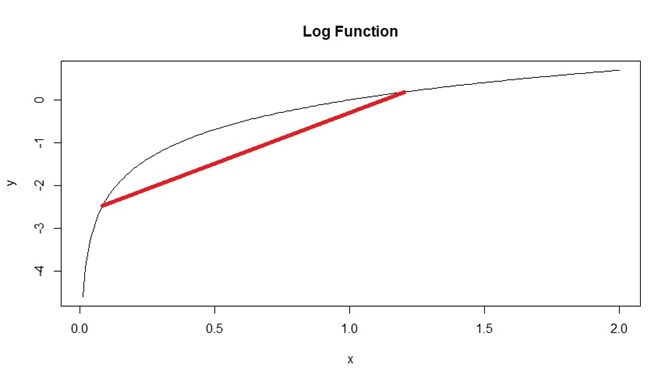
\includegraphics{images/06-concave.jpeg}
\caption{\label{fig:concave}Example of Concave Function}
\end{figure}

\begin{itemize}
\tightlist
\item
  \(g(x) = x^2\) is a convex function.

  \begin{itemize}
  \tightlist
  \item
    Its second derivative is \(g^{\prime \prime}(x) = 2\), which is always positive.
  \item
    We can also look at a graph of \(y = x^2\), and draw line segments that join two points on its graph. All of these lines are never below the graph. Figure \ref{fig:convex} below shows an example with one line segment, but we can see that any line segment that joins two points on the graph will never be velow the graph.
  \end{itemize}
\end{itemize}

\begin{figure}
\centering
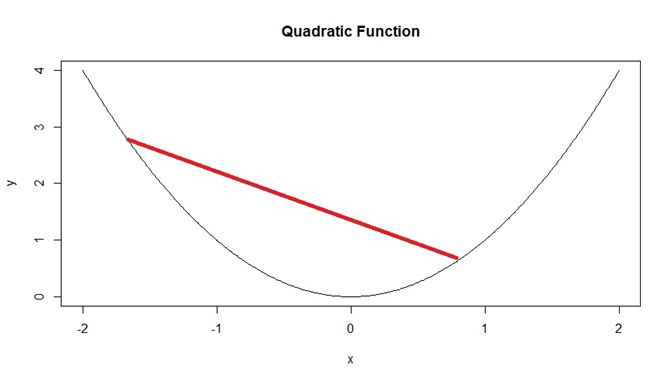
\includegraphics{images/06-convex.jpeg}
\caption{\label{fig:convex}Example of Convex Function}
\end{figure}

\emph{Thought question}: Consider the function \(g(x) = \frac{1}{x}\), i.e.~the inverse function. Can you explain why this function is convex when \(x>0\) and is concave when \(x<0\)?

\subsubsection{Jensen's Inequality}\label{jensens-inequality-1}

We are now ready to state \textbf{Jensen's inequality}. Let \(X\) denote a random variable. If \(g\) is convex, then \(E(g(X)) \geq g(E(X))\). If \(g\) is concave, then \(E(g(X)) \leq g(E(X))\).

The equality holds only if \(g\) is a linear function. It turns out linear functions are both convex and concave. The book goes through a simple proof of Jensen's inequality and is worth reading. Next, we apply Jensen's inequality to a few examples:

\begin{enumerate}
\def\labelenumi{\arabic{enumi}.}
\item
  We apply Jensen's inequality to the toy example in Section \ref{linnonlin}. As a reminder, suppose we roll a fair six-sided die, and let \(X\) denote the number of dots the die shows. The winnings is defined as the squared of the number of dots the die shows. Let \(T\) denote the new winnings, so \(T = X^2\), so \(g(x) = x^2\) is the function representing this non linear transformation. We established that the quadratic function is convex, so Jensen's inequality tells us that \(E(g(X)) \geq g(E(X))\), i.e.~that \(E(T) > E(X)^2\) which we showed in the code.
\item
  As mentioned in Section \ref{linnonlin}, a log transformation is often applied to make data that are right skewed less skewed, so that popular methods such as linear regression, tree based methods, \(K\) nearest neighbors can be used (these methods can be sensitive to outliers since they are based on conditional expectations or conditional means). What often happens is the log transformation is applied to the variable of interest, the model is fit, a prediction is made for the log transformed variable using conditional expectations, and the exponential is applied to this predicted value to convert it back to the original variable. Jensen's inequality tells us that the exponential of the average log variable is greater than the average variable, and our model over estimates.
\item
  Jensen's inequality can also be used to show that the sample standard deviation is a biased estimator of the population standard deviation, which appears counter intuitive, since the sample variance is an unbiased estimator of the population variance, i.e.~\(E(s^2) = \sigma^2\), but \(E(s) \neq \sigma\). The quick proof is
\end{enumerate}

\[
E(s) = E(\sqrt{s^2}) \leq \sqrt{E(s^2)} = \sigma.
\]

So the sample standard deviation underestimates the population standard deviation. However, this bias tends to be small if the sample size is large. We will cover ideas relating to unbiased estimators in a future module in more detail.

\subsection{Chebyshev's Inequality}\label{chebyshevs-inequality}

A common inequality that is used for probability is \textbf{Chebyshev's inequality}. It provides an upper bound on the probability that a random variable is at least a certain distance from its mean. Let \(X\) be a random variable with mean \(\mu\) and variance \(\sigma^2\). Then for any \(a>0\),

\begin{equation} 
P(|X-\mu| \geq a) \leq \frac{\sigma^2}{a^2}.
\label{eq:6-CI}
\end{equation}

An alternative way of expressing Chebyshev's inequality is to let \(a = c \sigma\) in equation \eqref{eq:6-CI}, so that it can be interpreted as providing an upper bound on the probability that a random variable is at least \(c\) standard deviations from its mean:

\begin{equation} 
P(|X-\mu| \geq c \sigma) \leq \frac{\sigma^2}{c^2 \sigma^2} = \frac{1}{c^2}.
\label{eq:6-CIalt}
\end{equation}

Using equation \eqref{eq:6-CIalt}, we can say the following about the upper bond on the probability that a random variable is at least 1, 2, and 3 standard deviations from its mean:

\begin{itemize}
\tightlist
\item
  When \(c=1\),
\end{itemize}

\[
P(|X-\mu| \geq \sigma) \leq \frac{1}{1^2} = 1.
\]
This informs us that the probability that a random variable is at least one standard deviation from its mean is no more than 1. The upper bound is not very informative in this setting since we know probabilities cannot be greater than 1.

\begin{itemize}
\tightlist
\item
  When \(c=2\),
\end{itemize}

\[
P(|X-\mu| \geq 2\sigma) \leq \frac{1}{2^2} = 0.25.
\]

This informs us the probability that a random variable is at least two standard deviations from its mean is no more than 0.25. In other words, there cannot be more than a 25\% chance that a random variable is at least 2 standard deviations from its mean, or there cannot be less than a 75\% chance that a random variable is within 2 standard deviations from its mean, since \(P(|X-\mu| \leq 2\sigma)\) is the complement of \(P(|X-\mu| \geq 2\sigma)\).

\begin{itemize}
\tightlist
\item
  When \(c=3\),
\end{itemize}

\[
P(|X-\mu| \geq 3\sigma) \leq \frac{1}{3^2} = \frac{1}{9}.
\]

There cannot be more than a 11.11\% chance that a random variable is at least 3 standard deviations from its mean, or there cannot be less than a 88.89\% chance that a random variable is within 3 standard deviations from its mean.

\emph{Thought question}: Can you explain how these results are consistent with the 68-99-99.7\% rule for normal distributions, as stated in Section \ref{rulenorm}?

Notice that Chebyshev's inequality can be applied to any distribution, and can be used to provide bounds on how data can be spread out. It is more flexible than the 68-99-99.7\% rule for normal distributions as it can be applied to any distribution, but the bounds are not as exact as they are an inequality. There can be a trade-off in relaxing assumptions and accuracy of results.

\section{Limit Theorems}\label{limits}

In the previous subsection, we used inequalities to provide bounds on probabilities and expectations that may be difficult to calculate. Another way of handing difficult calculations would be to use approximations for the distribution of the random variable, instead of the exact distribution of the random variable. Generally speaking, these approximations work better when we have more data (i.e.~when the sample size is larger). These approximations are covered by two of the most important limit theorems: the Law of Large Numbers and the Central Limit Theorem. These theorems approximate the distribution of the sample mean of i.i.d. (independent and identically distributed) random variables as the sample size gets larger.

Note: The idea of i.i.d. random variables implies that each observed value of the random variable is independent of each other, and that each observed value come from the same random variable. For example, let \(X\) denote the number of dots from a roll of a 6-sided fair die, and let \(X_1, X_2\) denote the value of the first and second roll respectively. \(X_1\) and \(X_2\) are i.i.d. since the outcomes from the first and second roll do not influence each other, so they are independent. \(X_1\) and \(X_2\) are identically distributed as they both follow the same distribution, \(Mult_6(1, (1/6, 1/6, 1/6, 1/6, 1/6, 1/6))\). In real life, this is achieved through carefully designed and planned surveys and experiments with random sampling, which is a whole field in statistics in its own right.

For the rest of this section, Section \ref{limits}, assume we have i.i.d. \(X_1, \cdots, X_n\) with finite mean \(\mu\) and finite variance \(\sigma^2\). For all positive integers \(n\) (i.e.~for any possible sample size), define the sample mean as \(\bar{X}_n = \frac{X_1 + \cdots + X_n}{n}\). We can easily derive the expected value and variance of the sample mean using properties of expectations and variances. Its expected value is

\begin{equation} 
\begin{split}
E(\bar{X}_n) &= E(\frac{X_1 + \cdots + X_n}{n}) \\
             &= \frac{1}{n}E(X_1 + \cdots + X_n) \\
             &= \frac{1}{n} (E(X_1) + \cdots + E(X_n)) \\
             &= \frac{1}{n} (\mu + \cdots + \mu) \\
             &= \mu.
\end{split}
\label{eq:6-Emean}
\end{equation}

Its variance is

\begin{equation} 
\begin{split}
Var(\bar{X}_n) &= Var(\frac{X_1 + \cdots + X_n}{n}) \\
             &= \frac{1}{n^2}Var(X_1 + \cdots + X_n) \\
             &= \frac{1}{n^2} (Var(X_1) + \cdots + Var(X_n)) \\
             &= \frac{1}{n^2} (\sigma^2 + \cdots + \sigma^2) \\
             &= \frac{\sigma^2}{n}.
\end{split}
\label{eq:6-Varmean}
\end{equation}

Equation \eqref{eq:6-Emean} informs us that the long-run average of sample means is equal to the population mean. We can imagine this if we had taken different random samples of size \(n\) from a population, and for each random sample we find the sample mean, and then average all these sample means. This average equals to the population mean \(\mu\). The code below provides a demonstration of these steps:

\begin{itemize}
\tightlist
\item
  We simulate a random sample of \(X_1, \cdots, X_{500}\) i.i.d. from standard normal.
\item
  Compute the sample mean and store it.
\item
  Repeat the previous steps for a total of 10 thousand reps.
\item
  Find the average of the 10 thousand sample means.
\end{itemize}

\begin{Shaded}
\begin{Highlighting}[]
\NormalTok{reps}\OtherTok{\textless{}{-}} \DecValTok{10000} \DocumentationTok{\#\#take 10000 random samples. This value should be large}
\NormalTok{n}\OtherTok{\textless{}{-}}\DecValTok{500} \DocumentationTok{\#\#sample size for each random sample}
\NormalTok{xbar}\OtherTok{\textless{}{-}}\FunctionTok{array}\NormalTok{(}\DecValTok{0}\NormalTok{,reps) }\DocumentationTok{\#\#store the sample mean for each random sample}

\FunctionTok{set.seed}\NormalTok{(}\DecValTok{90}\NormalTok{)}

\ControlFlowTok{for}\NormalTok{ (i }\ControlFlowTok{in} \DecValTok{1}\SpecialCharTok{:}\NormalTok{reps)}
  
\NormalTok{\{}
  
\NormalTok{  xbar[i]}\OtherTok{\textless{}{-}}\FunctionTok{mean}\NormalTok{(}\FunctionTok{rnorm}\NormalTok{(n)) }\DocumentationTok{\#\#find and store sample mean for each random sample}
  
\NormalTok{\}}

\FunctionTok{mean}\NormalTok{(xbar) }\DocumentationTok{\#\#average the sample means. This should be close to 0. }
\end{Highlighting}
\end{Shaded}

\begin{verbatim}
## [1] -0.0001034368
\end{verbatim}

Equation \eqref{eq:6-Varmean} informs us how to calculate the variance of the sample means. We can imagine this if we had taken different random samples of size \(n\) from a population, and for each random sample we find the sample mean, and then find the variance of all these sample means. It is the variance of the original random variable divided by \(n\). This means as the sample size gets larger, the variance of the sample means get smaller, in other words, the sample means tend to get closer to the population mean. We re run the code from above and also find the variance of the sample means.

\begin{Shaded}
\begin{Highlighting}[]
\NormalTok{reps}\OtherTok{\textless{}{-}} \DecValTok{10000} \DocumentationTok{\#\#take 10000 random samples. This value should be large}
\NormalTok{n}\OtherTok{\textless{}{-}}\DecValTok{500} \DocumentationTok{\#\#sample size for each random sample}
\NormalTok{xbar}\OtherTok{\textless{}{-}}\FunctionTok{array}\NormalTok{(}\DecValTok{0}\NormalTok{,reps) }\DocumentationTok{\#\#store the sample mean for each random sample}

\FunctionTok{set.seed}\NormalTok{(}\DecValTok{90}\NormalTok{)}

\ControlFlowTok{for}\NormalTok{ (i }\ControlFlowTok{in} \DecValTok{1}\SpecialCharTok{:}\NormalTok{reps)}
  
\NormalTok{\{}
  
\NormalTok{  xbar[i]}\OtherTok{\textless{}{-}}\FunctionTok{mean}\NormalTok{(}\FunctionTok{rnorm}\NormalTok{(n)) }\DocumentationTok{\#\#find and store sample mean for each random sample}
  
\NormalTok{\}}

\FunctionTok{mean}\NormalTok{(xbar) }\DocumentationTok{\#\#average the sample means. This should be close to 0. }
\end{Highlighting}
\end{Shaded}

\begin{verbatim}
## [1] -0.0001034368
\end{verbatim}

\begin{Shaded}
\begin{Highlighting}[]
\FunctionTok{var}\NormalTok{(xbar) }\DocumentationTok{\#\#variance of sample means. This should be close to 1/500, since n=500. }
\end{Highlighting}
\end{Shaded}

\begin{verbatim}
## [1] 0.001979948
\end{verbatim}

\subsection{Law of Large Numbers}\label{law-of-large-numbers}

The \textbf{Law of Large Numbers (LLN)} states that as \(n\) gets larger and approaches infinity, the sample mean \(\bar{X}_n\) converges to the true mean \(\mu\). This implies that the sample mean tends to get closer to the population mean with larger sample sizes. The key word here is tends to, it is not a guarantee that the sample mean always gets closer to the population mean whenever \(n\) gets larger, but it generally does. This explains why we tend to trust results from larger sample sizes.

Another implication of the LLN is that we can use simulations to verify theoretical results, since these results usually require us to simulate data based on a large number of independent replications.

The LLN is a by product of equations \eqref{eq:6-Emean} and \eqref{eq:6-Varmean}. Equation \eqref{eq:6-Varmean} informs us that as \(n\) gets larger, the variance of the sample mean gets smaller. Equation \eqref{eq:6-Emean} informs us that the sample mean is unbiased, i.e.~its long run average is equal to the true mean. Collectively, these inform us that as \(n\) gets larger, the sample mean is more likely to be closer to the true mean.

We use an example to illustrate the LLN, which comes from flipping a fair coin. Let \(X\) denote whether the coin lands heads or tails, and let \(X=1\) for heads and \(X=0\) for tails. We can say that \(X \sim Bern(0.5)\) since the coin is fair. Imagine flipping the coin \(n\) times, and record the outcome after each flip, so \(X_1, \cdots, X_n\) denote the outcome of each flip. We know that \(E(X) = 0.5\) since \(X \sim Bern(0.5)\). The LLN informs us that \(\bar{X}_1, \cdots, \bar{X}_n\) should usually get closer to 0.5 as \(n\) increases. In other words, the value of the sample proportion after each flip should get usually closer to 0.5 with more flips. The code below simulates this example for \(n=500\), and Figure \ref{fig:4-LLN2} shows how the sample proportions get closer to 0.5, in general.

\begin{Shaded}
\begin{Highlighting}[]
\NormalTok{n}\OtherTok{\textless{}{-}}\DecValTok{500} \DocumentationTok{\#\#make this big, but not too big otherwise picture is difficult to see}

\FunctionTok{set.seed}\NormalTok{(}\DecValTok{23}\NormalTok{)}

\NormalTok{X}\OtherTok{\textless{}{-}}\FunctionTok{rbinom}\NormalTok{(n,}\DecValTok{1}\NormalTok{,}\FloatTok{0.5}\NormalTok{) }\DocumentationTok{\#\#simulate 500 flips of fair coin}

\NormalTok{totals}\OtherTok{\textless{}{-}}\FunctionTok{cumsum}\NormalTok{(X) }\DocumentationTok{\#\#count total number of heads after each flip}
\NormalTok{index}\OtherTok{\textless{}{-}}\DecValTok{1}\SpecialCharTok{:}\NormalTok{n}
\NormalTok{props}\OtherTok{\textless{}{-}}\NormalTok{totals}\SpecialCharTok{/}\NormalTok{index }\DocumentationTok{\#\#find proportion of heads after each flip}

\DocumentationTok{\#\#create visual. LLN says that as n gets larger, the value of the sample proportion tends to get closer to 0.5}
\FunctionTok{plot}\NormalTok{(props, }\AttributeTok{type=}\StringTok{"l"}\NormalTok{, }\AttributeTok{main=}\StringTok{"Prop vs Sample Size"}\NormalTok{, }\AttributeTok{ylab=}\StringTok{"Proportion"}\NormalTok{, }\AttributeTok{xlab=}\StringTok{"n"}\NormalTok{)}
\FunctionTok{abline}\NormalTok{(}\AttributeTok{h=}\FloatTok{0.5}\NormalTok{, }\AttributeTok{col=}\StringTok{"blue"}\NormalTok{) }\DocumentationTok{\#\#overlay 0.5 for easy comparison}
\end{Highlighting}
\end{Shaded}

\begin{figure}
\centering
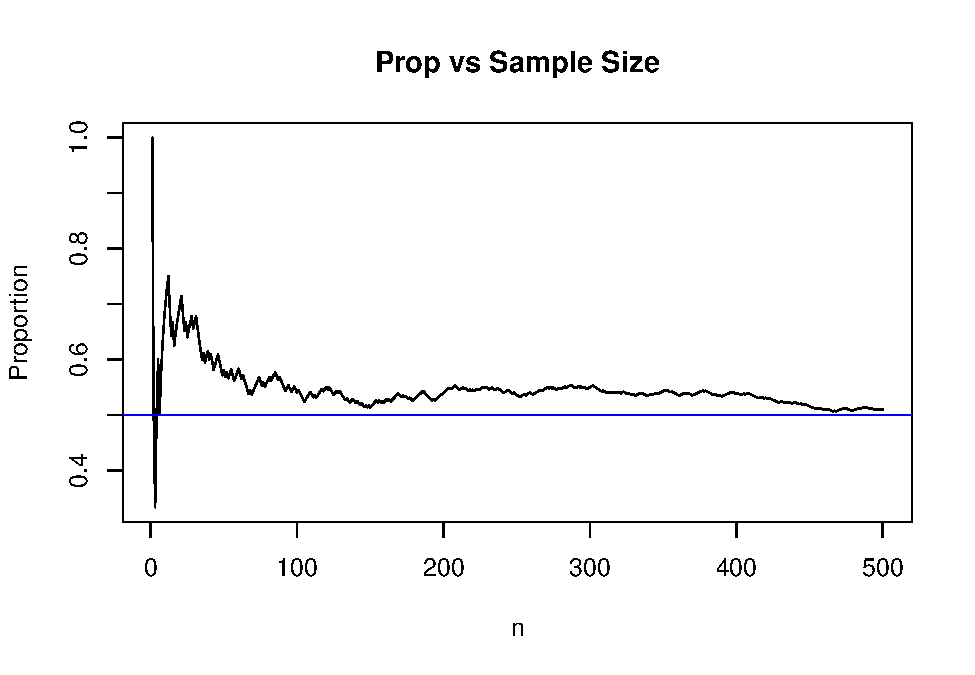
\includegraphics{bookdown-demo_files/figure-latex/4-LLN2-1.pdf}
\caption{\label{fig:4-LLN2}LLN Example 2}
\end{figure}

Note: \texttt{set.seed()} was used so you can reproduce these results exactly. However, the observation that the sample mean tends to get closer to the true mean as \(n\) increases will happen regardless of what \texttt{set.seed()} was used, or even if \texttt{set.seed()} was not used.

Note: The LLN actually comes in two versions, the Weak Law of Large Numbers (WLLN), and the Strong Law of Large Numbers (SLLN). The book goes into some detail about their definitions and differences. What I have written gives an intuitive explanation of what the LLN implies.

\subsubsection{Misconceptions with LLN}\label{misconceptions-with-lln}

One key idea with the LLN is that the sample mean \textbf{tends to get closer to the true mean as \(n\) gets larger}. The key words here are ``tends'' and ``as \(n\) gets larger''.

A misunderstanding of the LLN is the \textbf{gambler's fallacy}, which erroneously believes that the sample mean must ``self correct'' and get closer to the population mean with small increments of \(n\).

Using the example from flipping a fair coin. The gambler's fallacy erroneously thinks that:

\begin{itemize}
\tightlist
\item
  The proportion of heads should be close to 0.5, even with small \(n\).
\item
  The results of subsequent flips should self correct, i.e.~the proportion of heads get closer to 0.5 with the next flip. For example, if the first 5 flips are heads, the next flip is ``due'' to be tails since the proportion should get closer to 0.5 with the next flip.
\end{itemize}

The convergence to 0.5 comes from flipping the coin many times.

\subsection{Central Limit Theorem}\label{central-limit-theorem}

The LLN informs us that the sample mean converges to the true mean. Statistical theory informs us about the expected value and variance of the sample mean in equations \eqref{eq:6-Emean} and \eqref{eq:6-Varmean}. But these do not inform us about the distribution of \(\bar{X}_n\). This is where the \textbf{Central Limit Theorem (CLT)} comes in.

The CLT states that as the sample size gets larger and tends to infinity, the distribution of \(\bar{X}_n\) after standardization approaches a standard normal distribution, i.e.

\begin{equation} 
\sqrt{n} \left(\frac{\bar{X}_n \ - \mu}{\sigma} \right) \to N(0,1).
\label{eq:6-CLT}
\end{equation}

The CLT is called an \textbf{asymptotic} result, as it informs us about the \textbf{limiting distribution} of \(\bar{X}_n\) as \(n\) gets larger and tends to infinity. The CLT implies an approximation when \(n\) is large enough. For large \(n\), the distribution of \(\bar{X}_n\) is approximately \(N(\mu, \frac{\sigma^2}{n})\).

The implication of the CLT is that even if our data do not follow a normal distribution, the average value of the data can be approximated by a normal distribution if our sample size is large enough. As mentioned in Section \ref{normdist}, a lot of questions in research deal with averages.

We consider this hypothetical situation. Suppose the waiting time for customers calling customer service during lunch time is known have a mean of 600 seconds with standard deviation 30 seconds. The company decides to cut costs and reduces staffing at the call center, and claims that wait times are not affected negatively. The customers are convinced otherwise. A researchers obtains the wait times from 500 customers who call in during lunch time after staffing is reduced. The sample mean of the wait times for these customers is 700 seconds. Can this data be used to counter the company's claim that wait times have been affected?

One possible calculation will be to assume the company is. If so, the sample means will be approximately normal, with mean 600 and variance \(\frac{30}{\sqrt{500}}\), i.e.~\(\bar{X}_{500} \sim N(600, \frac{30^2}{\sqrt{500}})\). We then calculate \(P(\bar{X}_{500} \geq 700)\), the probability that we have sample mean that is equal to or greater than 700 seconds. Using R, this probability is about 0.0065, which is very small, indicating that our data is inconsistent with the company's claim.

\begin{Shaded}
\begin{Highlighting}[]
\DecValTok{1}\SpecialCharTok{{-}}\FunctionTok{pnorm}\NormalTok{(}\DecValTok{700}\NormalTok{, }\DecValTok{600}\NormalTok{, }\DecValTok{30}\SpecialCharTok{\^{}}\DecValTok{2}\SpecialCharTok{/}\FunctionTok{sqrt}\NormalTok{(}\DecValTok{500}\NormalTok{))}
\end{Highlighting}
\end{Shaded}

\begin{verbatim}
## [1] 0.006486311
\end{verbatim}

The CLT is traditionally associated with the distribution of the sample mean \(\bar{X}_n\). It can be applied to the sum as well, due to properties of expectations and variances. Let \(T_n = X_1 + \cdots + X_n = n \bar{X}_n\) denote the sum of \(n\) i.i.d. random variables. The CLT says that, for large \(n\), the distribution of \(T_n\) is approximately \(N(n\mu, n\sigma^2)\).

\subsubsection{Considerations with CLT}\label{considerations-with-clt}

One question that is raised when the CLT is used is how large does the sample size \(n\) have to be for the approximation to be accurate? While suggestions are plentiful (usually along the lines to sample size being at least 25 or 30), there is no fixed answer to this question. It depends on the distribution of \(X\). In general, the more skewed \(X\) is, \(n\) needs to be larger for the approximation to work. On the other hand, if \(X\) is already normal, then the distribution of \(\bar{X}_n\) is exactly \(N(\mu, \frac{\sigma^2}{n})\) for any sample size \(n\). We look at a couple of examples based on different distributions.

\begin{enumerate}
\def\labelenumi{\arabic{enumi}.}
\tightlist
\item
  \(X\) is standard normal. Our code will do the following:
\end{enumerate}

\begin{itemize}
\tightlist
\item
  We simulate \(n\) draws from \(X\) for \(n = 1\).
\item
  To obtain the distribution of \(\bar{X}_n\) for each value of \(n\), we repeat the previous step for a total of 10 thousand reps, then produce a histogram of the 10 thousand values of \(\bar{X}_n\).
\item
  Repeat the previous two steps, with different values of \(n\). We will use \(n= 5, 30, 100\) as well
\item
  We expect the histograms for \(\bar{X}_n\) to all look normal for all values of \(n\) we used.
\end{itemize}

\begin{figure}
\centering
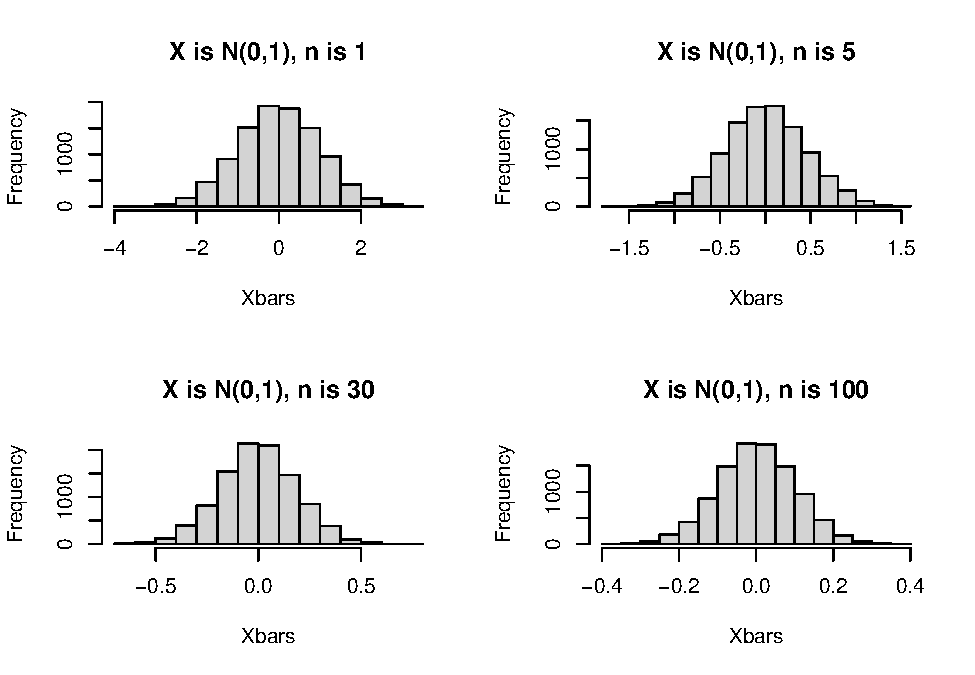
\includegraphics{bookdown-demo_files/figure-latex/6-CLTnorm-1.pdf}
\caption{\label{fig:6-CLTnorm}Distribution of Sample Means when X is N(0,1), n varied}
\end{figure}

Figure \ref{fig:6-CLTnorm} displays the histograms from this simulation, and matches what we expect from the CLT. Since \(X\) is normal, \(\bar{X}_n\) follows a normal distribution for any value of \(n\).

\begin{enumerate}
\def\labelenumi{\arabic{enumi}.}
\setcounter{enumi}{1}
\tightlist
\item
  \(X\) is Poisson with parameter 1. This is a skewed distribution. We use code that mimics the previous example, with the only difference being that our data are simulated from \(Pois(1)\) instead of standard normal. When \(n\) is small, we expect the distribution of \(\bar{X}_n\) to not look normal. As \(n\) gets larger, we expect the distribution of \(\bar{X}_n\) will look more normal.
\end{enumerate}

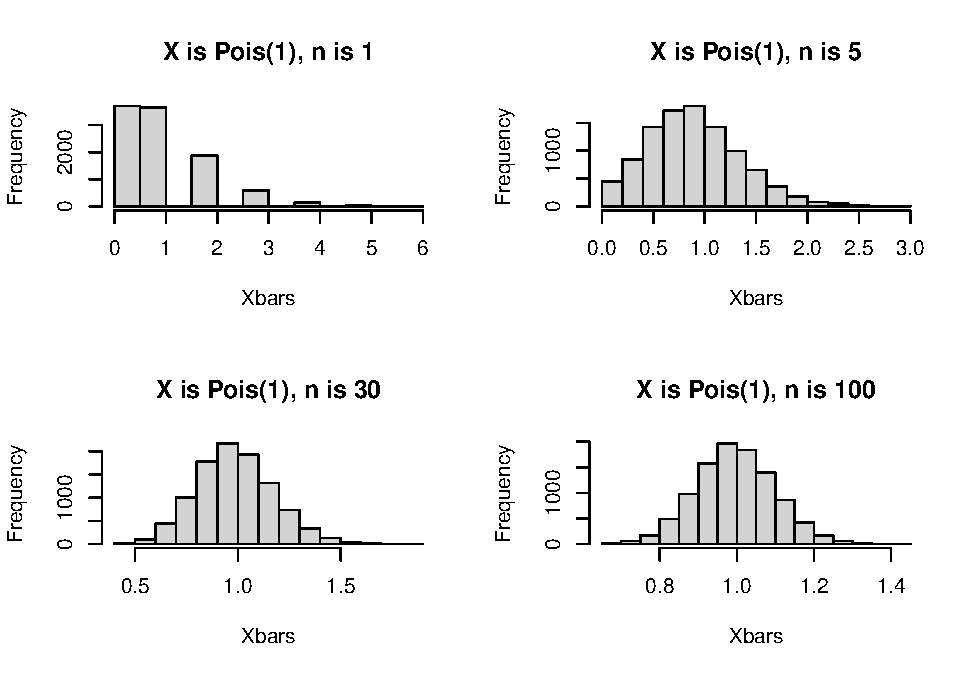
\includegraphics{bookdown-demo_files/figure-latex/6-CLTpois-1.pdf}
Figure \ref{fig:6-CLTpois} displays the histograms from this simulation, and matches what we expect. When \(n\) is 1 or 5, the histograms are clearly not normal, so the CLT approximation will not work well. When \(n=30\) the histogram looks approximately normal, and when \(n=100\), the histogram looks even closer to a normal distribution.

\section{Monte Carlo Simulations}\label{monte-carlo-simulations}

You may have that we have used simulations in the earlier sections of this module (and previous modules) to help explain certain concepts. These simulations are called \textbf{Monte Carlo} methods, or Monte Carlo simulations. The idea behind Monte Carlo methods is to used repeated random sampling (and by repeated, we mean repeat a large number of times) to estimate features of data, usually probabilities and expected values. Monte Carlo methods are used for the following purposes:

\begin{enumerate}
\def\labelenumi{\arabic{enumi}.}
\item
  When the probability or expectation is too complicated to work out by hand. Recall that finding probabilities and expectations by hand involve summations or integrals, and it becomes obvious that working with summations and especially integrals can get onerous.
\item
  To verify theoretical results involving probability or expectations. While a lot of theory is proved using mathematics, most academic papers include Monte Carlo simulations to verify the theoretical results. We have done these to verify the LLN and CLT in the previous subsection, in some circumstances.
\item
  To help confirm that you understand the meaning of theoretical results. The only way your code matches the theory is if you understand the theory.
\end{enumerate}

\subsection{Monte Carlo Methods for Expected Values}\label{monte-carlo-methods-for-expected-values}

Suppose we want to find some expectation for a continuous random variable \(X\), \(E(g(X))\), where \(g\) is some function. LOTUS says that we need to use equation \eqref{eq:4-lotus}, i.e.~\(E(g(X)) = \int_{-\infty}^{\infty} g(x) f_X(x).\) Monte Carlo methods avoid doing this integration by simulating \(X_1, \cdots, X_M\) from \(X\) and estimate \(E(g(X))\) with the sample mean of \(g(X)\), \(\frac{1}{M} \sum_{i=1}^M g(X_i)\). The LLN tells us that as \(M\) gets larger, this sample mean converges to \(E(g(X))\).

Monte Carlo methods replace the integral (or summation) with simulating a random variable repeatedly many times. We use a simple example to illustrate this idea.

Let \(X\) be a standard normal distribution. Suppose we want to find the value of \(E(X^2)\). If we try to find this using LOTUS, we will need to find \(\int_{-\infty}^{\infty} x^2 \frac{1}{\sqrt{2 \pi}} e^{-x^2/2} dx\). Instead of working out this integral by hand, we carry out a Monte Carlo simulation by doing these steps:

\begin{itemize}
\tightlist
\item
  Simulate \(M\) random values from a standard normal, where \(M\) is large.
\item
  Calculate \(X_1^2, \cdots, X_M^2\).
\item
  Find the sample average of \(X_1^2, \cdots, X_M^2\).
\end{itemize}

\begin{Shaded}
\begin{Highlighting}[]
\FunctionTok{set.seed}\NormalTok{(}\DecValTok{5}\NormalTok{)}

\NormalTok{reps}\OtherTok{\textless{}{-}}\DecValTok{10000} \DocumentationTok{\#\# this is M}

\NormalTok{Xs}\OtherTok{\textless{}{-}}\FunctionTok{rnorm}\NormalTok{(reps) }\DocumentationTok{\#\#generate M values of X}

\NormalTok{squared.values}\OtherTok{\textless{}{-}}\NormalTok{Xs}\SpecialCharTok{\^{}}\DecValTok{2} \DocumentationTok{\#\#square each X}

\FunctionTok{mean}\NormalTok{(squared.values) }\DocumentationTok{\#\#sample average of squared values. }
\end{Highlighting}
\end{Shaded}

\begin{verbatim}
## [1] 1.024546
\end{verbatim}

\begin{Shaded}
\begin{Highlighting}[]
\DocumentationTok{\#\#when reps is large, this sample mean should be close to the true E(X\^{}2), which is 1}
\end{Highlighting}
\end{Shaded}

Since \(X\) is standard normal, we know \(E(X) = 0\) and \(Var(X) = E(X^2) - E(X)^2 = E(X^2) = 1\). We see in our simulation that our estimated value for \(E(X^2)\) is pretty close to its theoretical value.

\subsection{Monte Carlo Methods for Probabilities}\label{monte-carlo-methods-for-probabilities}

Suppose we want to find the probability that a random variable satisfies some event \(E\), \(P(E)\). We could perform a summation or integral to find this probability, or estimate the probability using Monte Carlo methods. What we will do is simulate \(X_1, \cdots, X_M\) from \(X\), where \(M\) is large, in other words, simulate a large number of replicates of \(X\). We then count how many of the \(X_i\)s correspond to event \(E\) happening, and then divide this number by \(M\), the number of replicates. We use an example to illustrate this idea.

Let \(X\) be a standard normal distribution. Suppose we want to find the probability \(P(X^2 > 1)\). We carry out a Monte Carlo simulation by doing these steps:

\begin{itemize}
\tightlist
\item
  Simulate \(M\) random values from a standard normal, where \(M\) is large.
\item
  Calculate \(X_1^2, \cdots, X_M^2\).
\item
  Count the number of times \(X_i^2\) is greater than 1.
\item
  Divide this number by \(M\) to estimate the probability, since probability can be interpreted as a long-run proportion.
\end{itemize}

\begin{Shaded}
\begin{Highlighting}[]
\FunctionTok{set.seed}\NormalTok{(}\DecValTok{5}\NormalTok{)}

\NormalTok{reps}\OtherTok{\textless{}{-}}\DecValTok{10000} \DocumentationTok{\#\# this is M}

\NormalTok{Xs}\OtherTok{\textless{}{-}}\FunctionTok{rnorm}\NormalTok{(reps) }\DocumentationTok{\#\#generate M values of X}

\NormalTok{squared.values}\OtherTok{\textless{}{-}}\NormalTok{Xs}\SpecialCharTok{\^{}}\DecValTok{2} \DocumentationTok{\#\#square each X}

\FunctionTok{sum}\NormalTok{(squared.values}\SpecialCharTok{\textgreater{}}\DecValTok{1}\NormalTok{)}\SpecialCharTok{/}\NormalTok{reps }\DocumentationTok{\#\#count the number of times X\^{}2 is greater than 1, and divide by M}
\end{Highlighting}
\end{Shaded}

\begin{verbatim}
## [1] 0.3178
\end{verbatim}

\begin{Shaded}
\begin{Highlighting}[]
\DocumentationTok{\#\#when reps is large, this proportion should be close to}
\DecValTok{1}\SpecialCharTok{{-}}\FunctionTok{pchisq}\NormalTok{(}\DecValTok{1}\NormalTok{, }\AttributeTok{df=}\DecValTok{1}\NormalTok{)}
\end{Highlighting}
\end{Shaded}

\begin{verbatim}
## [1] 0.3173105
\end{verbatim}

\begin{Shaded}
\begin{Highlighting}[]
\DocumentationTok{\#\#it turns out that squaring a standard normal gives a chi{-}squared distribution with 1 df.}
\end{Highlighting}
\end{Shaded}

\subsection{Monte Carlo Methods for Other Purposes}\label{monte-carlo-methods-for-other-purposes}

Monte Carlo methods are not exclusively used estimating expected values and probabilities. They are versatile and can be used for a number of purposes, as long we need repeated random sampling.

A fun example that is pretty famous uses Monte Carlo simulations to estimate the value of \(\pi\). We can consider the following hypothetical dart throwing experiment to do so, based on the figure below:

\begin{figure}
\centering
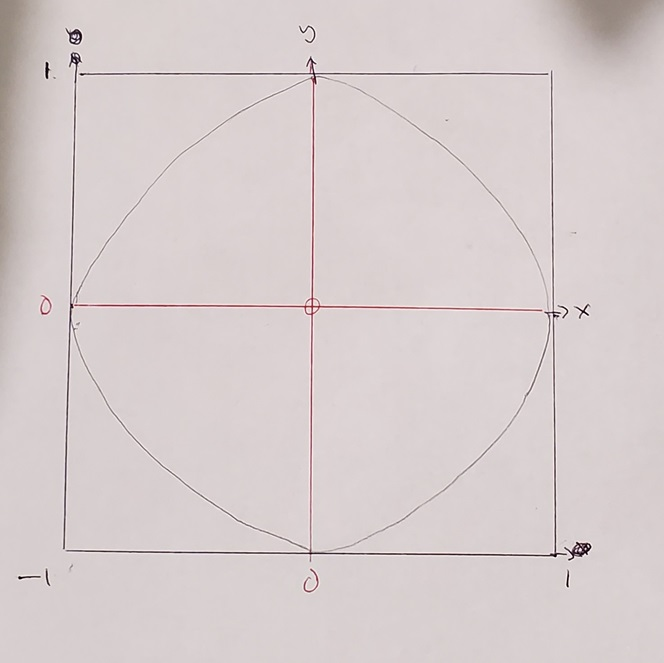
\includegraphics{images/06-circle.jpg}
\caption{\label{fig:circle}Board for Dart Throwing Experiment}
\end{figure}

The experiment works in this way:

\begin{itemize}
\tightlist
\item
  The dart will always land in the square, and has an equal probability of landing on any spot on the square.

  \begin{itemize}
  \tightlist
  \item
    We can let \(X \sim U(-1,1)\) to represent the position of the dart on the x-axis of the circle in Figure \ref{fig:circle}.
  \item
    We can let \(Y \sim U(-1,1)\) to represent the position of the dart on the y-axis of the circle in Figure \ref{fig:circle}.
  \end{itemize}
\item
  We will throw a large number of darts. For each dart, we will see if it lands in the circle or not.

  \begin{itemize}
  \tightlist
  \item
    To assess if a dart lies in the circle, we assess whether \(x_i^2 + y_i^2 \leq 1\) for dart \(i\). If this condition is met, we know dart \(i\) lies in the circle, if not, it lies outside the circle.
  \end{itemize}
\item
  It stands to reason that \(\frac{\text{Area of circle}}{\text{Are of square}} = \frac{\pi}{4} \approx \frac{\text{Number of darts landing in circle}}{\text{Number of darts thrown}}\).
\item
  Therefore, after throwing a large number of darts, \(\pi \approx 4 \times \frac{\text{Number of darts landing in circle}}{\text{Number of darts thrown}}.\)
\end{itemize}

The code below carries out this experiment with 10 thousand reps (or 10 thousand dart throws):

\begin{Shaded}
\begin{Highlighting}[]
\NormalTok{reps}\OtherTok{\textless{}{-}}\DecValTok{10000} \DocumentationTok{\#\#number of dart throws}

\NormalTok{count}\OtherTok{\textless{}{-}}\DecValTok{0} \DocumentationTok{\#\#counter that keeps track of number of throws inside circle}

\FunctionTok{set.seed}\NormalTok{(}\DecValTok{222}\NormalTok{)}

\ControlFlowTok{for}\NormalTok{ (i }\ControlFlowTok{in} \DecValTok{1}\SpecialCharTok{:}\NormalTok{reps) \{}

\NormalTok{x}\OtherTok{\textless{}{-}}\FunctionTok{runif}\NormalTok{(}\DecValTok{1}\NormalTok{,}\AttributeTok{min=}\SpecialCharTok{{-}}\DecValTok{1}\NormalTok{, }\AttributeTok{max=}\DecValTok{1}\NormalTok{) }\DocumentationTok{\#\#simulate landing spot on x axis}
\NormalTok{y}\OtherTok{\textless{}{-}}\FunctionTok{runif}\NormalTok{(}\DecValTok{1}\NormalTok{,}\AttributeTok{min=}\SpecialCharTok{{-}}\DecValTok{1}\NormalTok{, }\AttributeTok{max=}\DecValTok{1}\NormalTok{) }\DocumentationTok{\#\#simulate landing spot on y axis}

  \ControlFlowTok{if}\NormalTok{ (x}\SpecialCharTok{\^{}}\DecValTok{2} \SpecialCharTok{+}\NormalTok{ y}\SpecialCharTok{\^{}}\DecValTok{2} \SpecialCharTok{\textless{}=} \DecValTok{1}\NormalTok{)\{}
\NormalTok{    count }\OtherTok{\textless{}{-}}\NormalTok{ count}\SpecialCharTok{+}\DecValTok{1} \DocumentationTok{\#\#counter adds 1 if dart lands in circle}
\NormalTok{  \}}

\NormalTok{\}}

\DocumentationTok{\#\#estimate pi. should be close to real value of pi. Gets closer if we throw more darts}
\NormalTok{count}\SpecialCharTok{/}\NormalTok{reps }\SpecialCharTok{*} \DecValTok{4} 
\end{Highlighting}
\end{Shaded}

\begin{verbatim}
## [1] 3.1436
\end{verbatim}

\subsection{Considerations with Monte Carlo Methods}\label{considerations-with-monte-carlo-methods}

In the examples above, we compared estimated values using Monte Carlo methods with their real values, so we could see the methods work. However, if we do not know the real values, two questions will come to mind:

\begin{enumerate}
\def\labelenumi{\arabic{enumi}.}
\item
  How many replicates do we need? We only know the estimated values converge to the true values as we increase the number of replicates. Using more replicates will make the simulation run longer on your computer.
\item
  Related to the previous question, how close is close enough? How do you know your estimated value from the simulation is close enough to the truth? There is no way of knowing if the true value is unknown.
\end{enumerate}

\subsubsection{set.seed() in R}\label{set.seed-in-r}

You may have noticed that in the provided simulations, we use a function \texttt{set.seed()} called and input a number. This is to enable others to replicate the exact same results, if someone wants to verify the code.

With Monte Carlo simulations, we are generating numbers randomly. When we set the seed with \texttt{set.seed()} with a certain number, we ensure the same random numbers are generated each time the code is run.

We will not go into the details of how R generates the random numbers, and random number generation is a whole field in itself.

In terms of running the examples, you can choose to copy the code and exclude the line with \texttt{set.seed()}. You should still observe that the estimated values from the simulations are close to the true values.

  \bibliography{book.bib,packages.bib}

\end{document}
